% All fonts, including those for sub- and superscripts, must be 10
% points or larger.  Recommended sizes are 14-point for chapter
% headings, 12-point for the main body of text and figure/table
% titles, and 10-point for footnotes, sub- and super-scripts, and text
% in figures and tables.
%
% Notes: Add short title to figures, sections, via square brackets,
% e.g. \section[short]{long}.
%
%\documentclass[12pt,fleqn]{style/ucithesis}
\documentclass[11pt]{style/ucithesis}

% A few common packages
\usepackage{amsmath}
\usepackage{amsthm}
\usepackage{amssymb}
\usepackage{array}
\usepackage{graphicx}
\usepackage{relsize}
\usepackage{geometry}

% Some other useful packages
\usepackage{caption}
\usepackage{subcaption}  % \begin{subfigure}...\end{subfigure} within figure
\usepackage{multirow}
\usepackage{tabularx}
\usepackage{gensymb}
\usepackage{bm}
\usepackage{slashed}
%\usepackage{makecell}
%\usepackage{cellspace}
\usepackage{braket}
\usepackage{lineno}
%\linenumbers

% plainpages=false fixes the "duplicate ignored" error with page counters
% Set pdfborder to 0 0 0 to disable colored borders around PDF hyperlinks
\usepackage[plainpages=false,pdfborder={0 0 0}]{hyperref}
\usepackage{epigraph}
\setlength{\epigraphwidth}{0.8\textwidth}
\setlength\epigraphrule{0pt}

\usepackage[sorting=none,hyperref,backend=biber,backref,backrefstyle=none]{biblatex}
\bibliography{bib/references.bib,
                bib/sm_final.bib,
                bib/chapter2.bib,
                bib/bsm.bib,
                bib/chapter3.bib,
                bib/simulation.bib,
                bib/nsw.bib,
                bib/common_ana.bib,
                bib/general.bib,
                bib/systematics.bib,
                bib/stats_hypo.bib,
                bib/stop2l.bib,
                bib/bbll.bib,
                bib/conclusion.bib,
                bib/previous_theses.bib
}

\usepackage{tabularx}
\usepackage{booktabs}

\usepackage{array}
\usepackage{makecell}
\usepackage{graphicx}
\usepackage{arydshln}
\usepackage{stackengine}
\usepackage{xcolor}
\usepackage{amsmath}
\usepackage{placeins}
\usepackage{mathtools}


%\usepackage[sorting=none]{biblatex}
%\addbibresource{bib/references.bib}

% Uncomment the following two lines to use the algorithm package,
% which provides an algorithm environment similar to figure and table
% ("\begin{algorithm}...\end{algorithm}"). A list of algorithms will
% automatically be added in the preliminary pages. Note that you
% probably want a package for the actual code to go with this (e.g.,
% algorithmic).
%\usepackage{algorithm}
%\renewcommand{\listalgorithmname}{\protect\centering\protect\Large LIST OF ALGORITHMS}

% Uncomment the following line to enable Unicode support. This will allow you
% to enter non-ASCII characters (such as accented characters) directly without
% having to use LaTeX's awkward escape syntax (e.g., \'{e})
% NOTE: You may have to install the ucs.sty package for this to work. See:
% http://www.unruh.de/DniQ/latex/unicode/
%\usepackage[utf8x]{inputenc}

% Uncomment the following to avoid "widowing", where page breaks cause
% single lines of paragraphs to float onto the next page (this is not
% a UCI requirement but more of an aesthetic choice).
%\widowpenalty=10000
%\clubpenalty=10000

% Modify or extend these at will.
\newtheorem{theorem}{\textsc{Theorem}}[chapter]
\newtheorem{definition}{\textsc{Definition}}[chapter]
\newtheorem{example}{\textsc{Example}}[chapter]

% Macros for title, author, abstract, etc.
%\thesistitle{
%    Sweet Little Nothings: Searching for a Pairs of Supersymmetric Tops,
%        a Pair of Higgs Bosons, and a Pair of New Small Wheels for the 
%        Upgrade of the ATLAS Forward Muon System
%}

\thesistitle{
Searches for Anomalous Resonances in the Large Hadron Collider for New Physics
}

%"Dissertation" for PhD, "Thesis" for master's
\documenttitle{Dissertation}

\degreename{Doctor of Philosophy}

% Use the wording given in the official list of degrees awarded by UCI:
% http://www.rgs.uci.edu/grad/academic/degrees_offered.htm
\degreefield{
Physics
}

% Your name as it appears on official UCI records.
\authorname{
Yvonne Ng
}

% Use the full name of each committee member.
\committeechair{Professor Daniel Whiteson}
\othercommitteemembers
{
  Professor Tim Tait\\
  Professor Andrew Lankford
}

\degreeyear{2021}

\copyrightdeclaration
{
  {\copyright} {\Degreeyear} \Authorname
}

% If you have previously published parts of your manuscript, you must list the
% copyright holders; see Section 3.2 of the UCI Thesis and Dissertation Manual.
% Otherwise, this section may be omitted.
% \prepublishedcopyrightdeclaration
% {
% 	Chapter 4 {\copyright} 2003 Springer-Verlag \\
% 	Portion of Chapter 5 {\copyright} 1999 John Wiley \& Sons, Inc. \\
% 	All other materials {\copyright} {\Degreeyear} \Authorname
% }

% The dedication page is optional
% (comment out to exclude).
\dedications
{
  (Optional dedication page)
  
  To ...
}

\acknowledgments
{
    %That ``we don't accomplish anything in this world alone'' is never more true than in the
case of attempting a doctorate in physics, especially in the sub-field of experimental
high energy particle physics that, nowadays, likely has you stretched across the globe
in your work on large-scale experiments operated by international collaborations.

I have had the opportunity to be based at CERN for essentially the entirety of my doctorate.
This would not have been possible without the many people who have helped me along the way.
Their number is many, too far to count or list here.
They know who they are, though, and without them I would not have succeeded.
Not professionally and most definitely not personally.

As a result, the importance of my friends and family has never felt stronger.
Without them none of this means a thing and I am surely indebted to them forever.
They have given me the opportunity to climb mountains (figuratively and literally), not feel alone in the world,
and to establish a true home in France and Switzerland.
The pain and suffering that a young researcher sometimes feels, whether in pushing out a physics analysis or in confronting the
rather unscientific bureaucracies inherent in a large collaboration like ATLAS, are far outweighed by their measure.
The biggest takeaways from my time at CERN are therefore not technical at all and boil down to
a few of the ``strongest of all warriors'' that are requisite in our dealings and goings-on about
the world: patience and compassion.
I have been damn lucky to have been surrounded by exemplars of these two during my doctorate.
I hope to follow along in their footsteps as we move forward.

Also thanks to Dan.

     First of all, I would like to thank my advisor Daniel Whiteson and Andy Lankford for the guidance, support, trust, and freedom they have given me over the years. I am especially grateful for Daniel's continuous encouragement towards my growth into an independent researcher. 

I would also like to thank my postdocs Dan Guest and Mike Fenton. Thank you for all the big and small advice on my work and personal encouragements over the years- sometime in the form of French Kabob runs or pandemic zoom coffees sessions. A special thank you is also dedicated to Kate Pachal, for your generous support through my first major analysis, for teaching me so much that I know now, and for the afternoon cake time at R1. I will strive to be like what you all were to me to my future students.

I am grateful for my colleagues at CERN, especially Verena Martinez, Bill Murray, Ben Nachman, Bogdan Malaescu, Caterina Doglioni, Christopher Haynes, Ljiljana Morvaj, Heather Russell, and Kyle Cranmer. The end product of this thesis would not have the same rigor without your technical comments and contributions.

A gratitude is also extended to my informal advisors in Irvine, Tim Tait, Muchun Chen, Simona Murgia, and Michael Ratz for the intellectual support and advice. I also want to thank Flip Tanedo for all the coffee and restaurant runs in my first two years of grad school. I was nourished in the mind, in my stomach, and also in my caffeine level. I also want to thank Chase and Seyda for all the thought-provoking chats.

If I am allowed the indulgence to take it back to where the journey begins, I want to thank my middle science teacher Miss Chau, thank you for always having so much trust in my abilities and for showing me how practical and relatable science is. I also want to thank my math teacher Miss Fung: for both the lessons in math and outside of math. Some words outside of math took me many years more years to understand after class was over. I am grateful to my undergraduate friends and
``Senpais" David and Jason, for showing me the fun of solving technical problems with science and engineering and for being great friends. I am also thankful for research time from MC Chu in his lab. I learned not just the rigor of scientific research but also responsibility as a scientist to society. I aspire to continue my efforts of scientific outreach as a postdoc like you have done for so many. 

%NAthan , Chase, seyda matt and jennifer, 
It only took 3 continents to finish my Ph.D. These would not have been possible without the support of my friends across all three continents. Special shout out to Andy, Clare, Diane, Haidee, Alexis, Ros, Yanyi, CY, Rhoda, Alice, Joakim, Lily, Arianna, Freida, Kit, Ho, Amber, Tamara, Kiwi, Shelly, Danny, friends in Kindle Hills. My life in the last few years both instead and outside of physics really wouldn't have been the same without you.

Finally to my family: mom and dad, I hope I made you proud. To my brother Rene, I am lucky to have your support and to have you as a partner in crime through all of life's adventures.

This thesis is for all of you.


%  I would like to thank...
%  
%  (You must acknowledge grants and other funding assistance. 
%  
%  You may also acknowledge the contributions of professors and
%  friends.
%  
%  You also need to acknowledge any publishers of your previous
%  work who have given you permission to incorporate that work
%  into your dissertation. See Section 3.2 of the UCI Thesis and
%  Dissertation Manual.)
}


% Some custom commands for your list of publications and software.
\newcommand{\mypubentry}[3]{
  \begin{tabular*}{1\textwidth}{@{\extracolsep{\fill}}p{4.5in}r}
    \textbf{#1} & \textbf{#2} \\ 
    \multicolumn{2}{@{\extracolsep{\fill}}p{.95\textwidth}}{#3}\vspace{6pt} \\
  \end{tabular*}
}
\newcommand{\mysoftentry}[3]{
  \begin{tabular*}{1\textwidth}{@{\extracolsep{\fill}}lr}
    \textbf{#1} & \url{#2} \\
    \multicolumn{2}{@{\extracolsep{\fill}}p{.95\textwidth}}
    {\emph{#3}}\vspace{-6pt} \\
  \end{tabular*}
}

% Include, at minimum, a listing of your degrees and educational
% achievements with dates and the school where the degrees were
% earned. This should include the degree currently being
% attained. Other than that it's mostly up to you what to include here
% and how to format it, below is just an example.
%
% CV is required for PhD theses, but not Master's
% comment out to exclude
\curriculumvitae
{
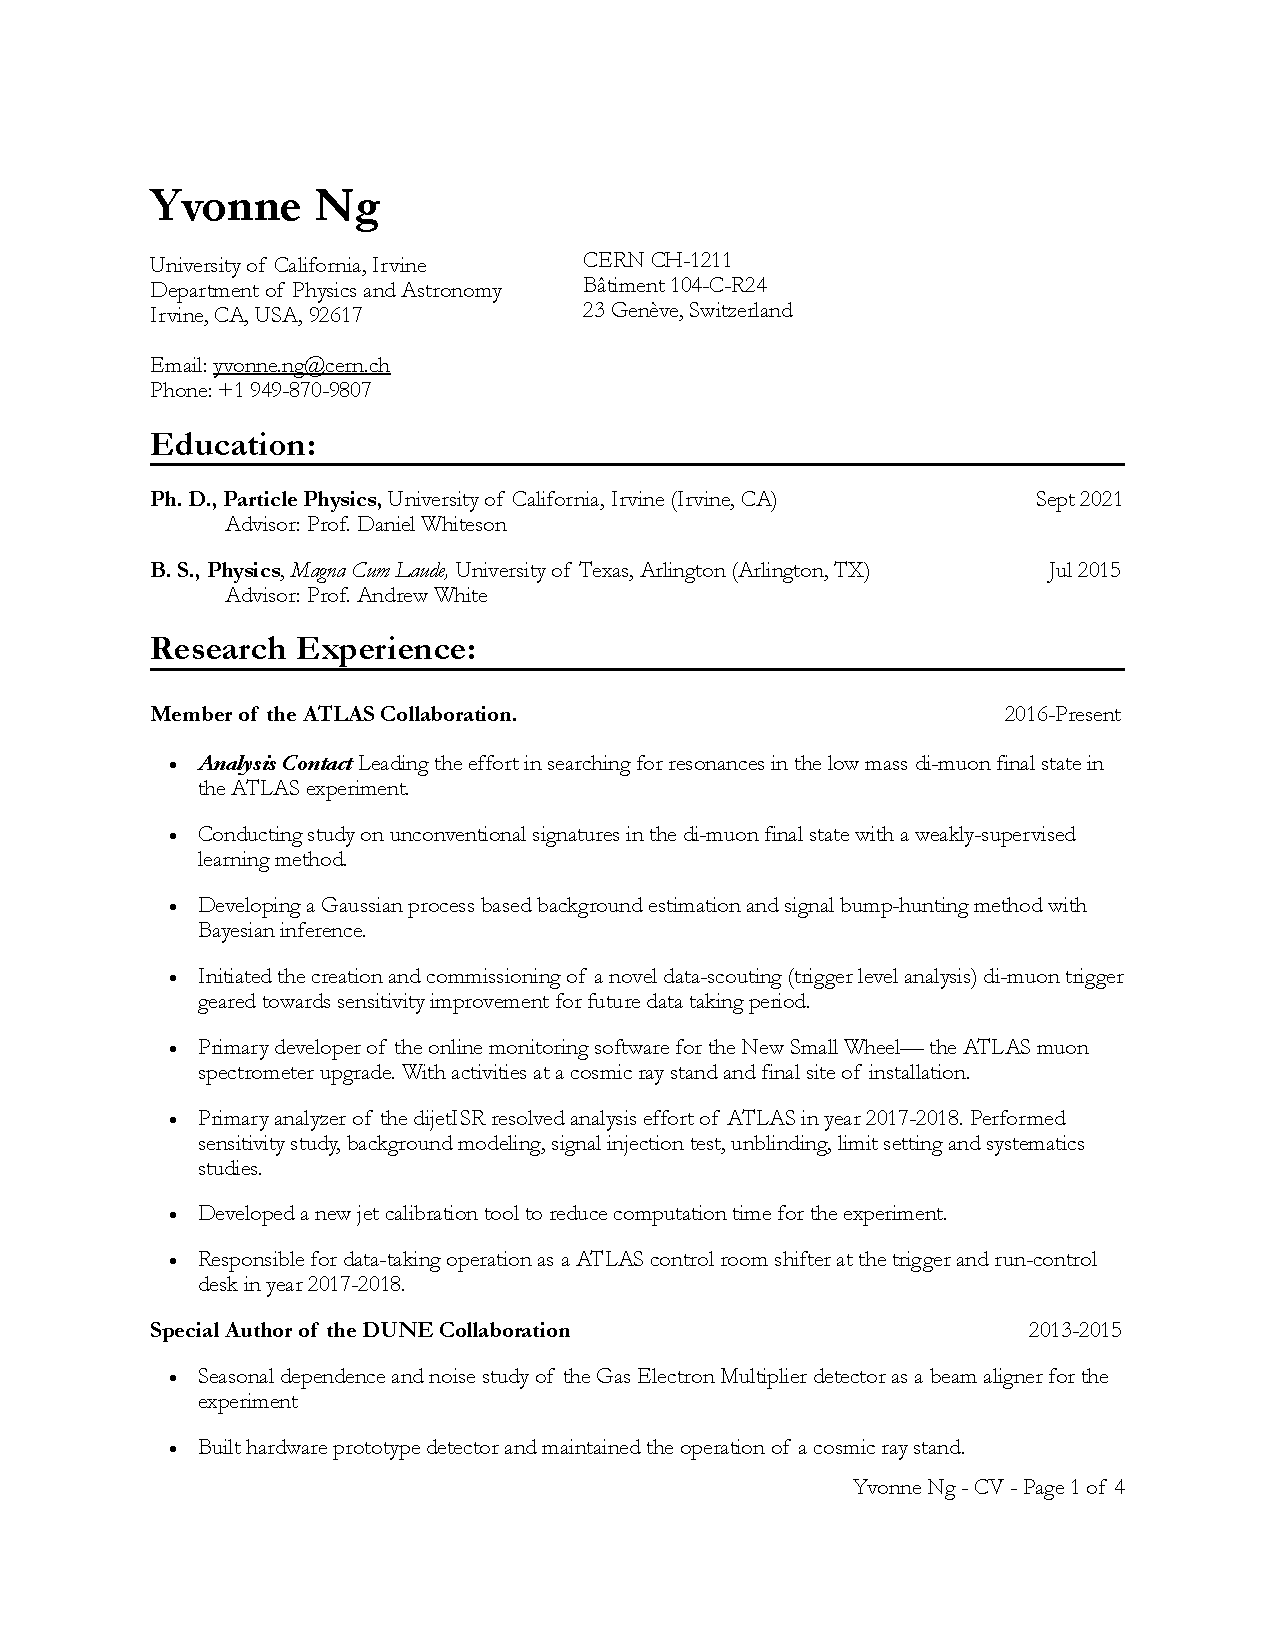
\includepdf[pages=-]{/Users/yvonne/WorkSpace/phd_thesis/phd_thesis/thesis/misc_metadata/cv/YWYvonneNg_CV_FermiLab.pdf}



%\textbf{EDUCATION}
%  
%  \begin{tabular*}{1\textwidth}{@{\extracolsep{\fill}}lr}
%    \textbf{Doctor of Philosophy in Computer Science} & \textbf{2012} \\
%    \vspace{6pt}
%    University name & \emph{City, State} \\
%    \textbf{Bachelor of Science in Computational Sciences} & \textbf{2007} \\
%    \vspace{6pt}
%    Another university name & \emph{City, State} \\
%  \end{tabular*}
%
%\vspace{12pt}
%\textbf{RESEARCH EXPERIENCE}
%
%  \begin{tabular*}{1\textwidth}{@{\extracolsep{\fill}}lr}
%    \textbf{Graduate Research Assistant} & \textbf{2007--2012} \\
%    \vspace{6pt}
%    University of California, Irvine & \emph{Irvine, California} \\
%  \end{tabular*}
%
%\vspace{12pt}
%\textbf{TEACHING EXPERIENCE}
%
%  \begin{tabular*}{1\textwidth}{@{\extracolsep{\fill}}lr}
%    \textbf{Teaching Assistant} & \textbf{2009--2010} \\
%    \vspace{6pt}
%    University name & \emph{City, State} \\
%  \end{tabular*}
%
%\pagebreak
%
%\textbf{REFEREED JOURNAL PUBLICATIONS}
%
%  \mypubentry{Ground-breaking article}{2012}{Journal name}
%
%\vspace{12pt}
%\textbf{REFEREED CONFERENCE PUBLICATIONS}
%
%  \mypubentry{Awesome paper}{Jun 2011}{Conference name}
%  \mypubentry{Another awesome paper}{Aug 2012}{Conference name}
%
%\vspace{12pt}
%\textbf{SOFTWARE}
%
%  \mysoftentry{Magical tool}{http://your.url.here/}
%  {C++ algorithm that solves TSP in polynomial time.}
%
}

% The abstract was previously limited to a maximum of 350 words, 
% but the UCI manual at https://etd.lib.uci.edu/electronic/td2e#2.2.1.
% currently does not indicate that there is any word limit for the abstract
\thesisabstract
{
  Many empirical evidence points to the existence of beyond-the-standard-model physics. In the LHC, different theoretical and experiemntal tehcniques are used to look for new particles as for new physics. One method with theoretical elegance and clean experimental reconstruction, is the resonance finding method. The method has enjoyed much sucesses in the past, W, Z and the Higgs boson are some of the few particles discovered this way. However, the early beyond-the-standard-model resonance search program of the LHC has returned empty handed. 
In this thesis, I ask the question of whether the standard approach could be modified to look for "weird resonances", particles that exist in the LHC dataset but goes beyond the standard program. Their discovery can provide important clue to beyond-the-standard-model physics. 

Three physics analyses beyond the usual search program are covered in this thesis. The first two on the dijetISR final state and the last one on dimuon final state. In the dijetISR searches, an ISR object is used to boost the final state. By triggering on the ISR object rather than the resonance formming final state, lower mass resonances can be covered. These two analysis set the lowest ATLAS low mass limit below the standard dijet search. In the dimuon search, as previous searches has neglected the low mass region below the Z peak, the search seeks to cover the region from 12-70 GeV. A novel statistical method driven by Gaussian Process is used. The method allow for a simple background estimation for a similar class of future analyses where Monte Carlo is limited.

All of these analyses provide competitive exclusion in the dark matter benchmark model of the LHC in places not previously covered.

As a future discussion, a new stream from trigger level analysis could be implemented to the dimuon search to improve the low mass sensitivity. Data driven approach like CWOLA can also be used to look for resonances free of an assumed signal model.

The thesis also covers involvement jet in-situ calibration as well as the new small wheel online monitoring software development.

"Weird resonances" are the "out-of-ordinary" ones: They are not a part of the current knowledge model; they break existing laws; they defies our knowledge about the world and human-beings; they are already somewhere out there, but only from its discovery it can be realized that we are more than what we think we are. The search for weird resonanances is a search for authenticity.

  %The abstract of your contribution goes here.
}


%%% Local Variables: ***
%%% mode: latex ***
%%% TeX-master: "thesis.tex" ***
%%% End: ***


% Add PDF document info fields
\hypersetup{
	pdftitle={\Thesistitle},
	pdfauthor={\Authorname},
	pdfsubject={\Degreefield},
}

% Uncomment the following to have numbered subsubsections (by default
% numbering goes only to subsections).
%\setcounter{secnumdepth}{4}


% Set this to only select a subset of the includes directives below.
% Very handy to speed up compilation if you're working on a certain
% part of your thesis. It conserves page numbers, references, etc.
% even for non-included files.

%% commands
\newcommand{\SUewk}{$\mathcal{SU}(2)_{L} \times \mathcal{U}(1)_{Y}$}
\newcommand*{\Uone}{$\mathcal{U}(1)$}
\newcommand{\SUtwo}{$\mathcal{SU}(2)$}
\newcommand{\SUthree}{$\mathcal{SU}(3)$}

\newcommand{\SML}{$\mathcal{L}_{\text{SM}}$}
\newcommand{\fieldQi}{$Q_i$}
\newcommand{\fieldUri}{$u_{\text{R},i}$}
\newcommand{\fieldDri}{$d_{\text{R},i}$}
\newcommand{\fieldLi}{$L_i$}
\newcommand{\fieldEri}{$e_{\text{R},i}$}
\newcommand{\fieldB}{$B$}
\newcommand{\fieldW}{$W$}
\newcommand{\fieldWone}{$W_1$}
\newcommand{\fieldWtwo}{$W_2$}
\newcommand{\fieldWthree}{$W_3$}
\newcommand{\fieldWp}{$W^+$}
\newcommand{\fieldWm}{$W^-$}
\newcommand{\fieldWzero}{$W^0$}
\newcommand{\fieldWpm}{$W^{\pm}$}
\newcommand{\fieldZ}{$Z$}
\newcommand{\fieldZzero}{$Z^0$}
\newcommand{\fieldPhoton}{$\gamma$}
\newcommand{\fieldG}{$G$}
\newcommand{\quarkU}{$u$}
\newcommand{\quarkD}{$d$}
\newcommand{\quarkC}{$c$}
\newcommand{\quarkS}{$s$}
\newcommand{\quarkT}{$t$}
\newcommand{\quarkB}{$b$}
\newcommand{\leptonE}{$e$}
\newcommand{\leptonMu}{$\mu$}
\newcommand{\leptonTau}{$\tau$}
\newcommand{\neutrinoE}{$\nu_e$}
\newcommand{\neutrinoMu}{$\nu_{\mu}$}
\newcommand{\neutrinoTau}{$\nu_{\tau}$}
\newcommand{\fieldUl}{$u_{\text{L}}$}
\newcommand{\fieldDl}{$d_{\text{L}}$}
\newcommand{\fieldCl}{$c_{\text{L}}$}
\newcommand{\fieldSl}{$s_{\text{L}}$}
\newcommand{\fieldTl}{$t_{\text{L}}$}
\newcommand{\fieldBl}{$b_{\text{L}}$}
\newcommand{\fieldUr}{$u_{\text{R}}$}
\newcommand{\fieldDr}{$d_{\text{R}}$}
\newcommand{\fieldCr}{$c_{\text{R}}$}
\newcommand{\fieldSr}{$s_{\text{R}}$}
\newcommand{\fieldTr}{$t_{\text{R}}$}
\newcommand{\fieldBr}{$b_{\text{R}}$}
\newcommand{\fieldEl}{$e_{\text{L}}$}
\newcommand{\fieldMul}{$\mu_{\text{L}}$}
\newcommand{\fieldTaul}{$\tau_{\text{L}}$}
\newcommand{\fieldEr}{$e_{\text{R}}$}
\newcommand{\fieldMur}{$\mu_{\text{R}}$}
\newcommand{\fieldTaur}{$\tau_{\text{R}}$}
\newcommand{\fieldNuEl}{$\nu_{e,\text{L}}$}
\newcommand{\fieldNuMul}{$\nu_{\mu,\text{L}}$}
\newcommand{\fieldNuTaul}{$\nu_{\tau,\text{L}}$}
\newcommand{\fieldNuR}{$\nu_{\text{R}}$}
\newcommand{\fieldPhi}{$\mathcal{\phi}$}
\newcommand{\fieldPhip}{$\mathcal{\phi}^+$}
\newcommand{\fieldPhizero}{$\mathcal{\phi}^0$}
\newcommand{\fieldH}{$h$}
\newcommand*{\TeV}{\ensuremath{\text{Te\kern -0.1em V}}}
\newcommand*{\GeV}{\ensuremath{\text{Ge\kern -0.1em V}}}
\newcommand*{\MeV}{\ensuremath{\text{Me\kern -0.1em V}}}
\newcommand*{\pT}{\ensuremath{p_{T}}}
\newcommand*{\micron}{\ensuremath{\mu m}}

\usepackage{xspace}
\newcommand*{\ptmiss}{\ensuremath{\mathbf{p}_{\text{T}}^{\text{miss}}}\xspace}
\newcommand*{\met}{\ensuremath{E_{\text{T}}^{\text{miss}}}\xspace}
\newcommand*{\antikt}{\ensuremath{\text{anti-}k_t}\xspace}
\newcommand*{\npv}{\ensuremath{N_{\text{PV}}}\xspace}

\newcommand*{\micromegas}{MicroMegas\xspace}
\newcommand*{\stgc}{sTGC\xspace}

\newcommand*{\ttbar}{\ensuremath{t\bar{t}}}
\newcommand*{\wt}{\ensuremath{Wt}}
\newcommand*{\zhf}{$Z$+HF}
\newcommand*{\vv}{\ensuremath{VV}}
\newcommand*{\cls}{\ensuremath{\text{CL}_{\text{s}}}\xspace}

% BSM

\newcommand*{\nino}{\ensuremath{\mathchoice%
      {\displaystyle\raise.4ex\hbox{$\displaystyle\tilde\chi^0$}}%
         {\textstyle\raise.4ex\hbox{$\textstyle\tilde\chi^0$}}%
       {\scriptstyle\raise.3ex\hbox{$\scriptstyle\tilde\chi^0$}}%
 {\scriptscriptstyle\raise.3ex\hbox{$\scriptscriptstyle\tilde\chi^0$}}}\xspace}
\newcommand*{\ninoone}{\ensuremath{\mathchoice%
      {\displaystyle\raise.4ex\hbox{$\displaystyle\tilde\chi^0_1$}}%
         {\textstyle\raise.4ex\hbox{$\textstyle\tilde\chi^0_1$}}%
       {\scriptstyle\raise.3ex\hbox{$\scriptstyle\tilde\chi^0_1$}}%
 {\scriptscriptstyle\raise.3ex\hbox{$\scriptscriptstyle\tilde\chi^0_1$}}}\xspace}
\newcommand*{\ninotwo}{\ensuremath{\mathchoice%
      {\displaystyle\raise.4ex\hbox{$\displaystyle\tilde\chi^0_2$}}%
         {\textstyle\raise.4ex\hbox{$\textstyle\tilde\chi^0_2$}}%
       {\scriptstyle\raise.3ex\hbox{$\scriptstyle\tilde\chi^0_2$}}%
 {\scriptscriptstyle\raise.3ex\hbox{$\scriptscriptstyle\tilde\chi^0_2$}}}\xspace}
\newcommand*{\ninothree}{\ensuremath{\mathchoice%
      {\displaystyle\raise.4ex\hbox{$\displaystyle\tilde\chi^0_3$}}%
         {\textstyle\raise.4ex\hbox{$\textstyle\tilde\chi^0_3$}}%
       {\scriptstyle\raise.3ex\hbox{$\scriptstyle\tilde\chi^0_3$}}%
 {\scriptscriptstyle\raise.3ex\hbox{$\scriptscriptstyle\tilde\chi^0_3$}}}\xspace}
\newcommand*{\ninofour}{\ensuremath{\mathchoice%
      {\displaystyle\raise.4ex\hbox{$\displaystyle\tilde\chi^0_4$}}%
         {\textstyle\raise.4ex\hbox{$\textstyle\tilde\chi^0_4$}}%
       {\scriptstyle\raise.3ex\hbox{$\scriptstyle\tilde\chi^0_4$}}%
 {\scriptscriptstyle\raise.3ex\hbox{$\scriptscriptstyle\tilde\chi^0_4$}}}\xspace}
\newcommand*{\chinoonep}{\ensuremath{\mathchoice%
      {\displaystyle\raise.4ex\hbox{$\displaystyle\tilde\chi^+_1$}}%
         {\textstyle\raise.4ex\hbox{$\textstyle\tilde\chi^+_1$}}%
       {\scriptstyle\raise.3ex\hbox{$\scriptstyle\tilde\chi^+_1$}}%
 {\scriptscriptstyle\raise.3ex\hbox{$\scriptscriptstyle\tilde\chi^+_1$}}}\xspace}
\newcommand*{\chinoonem}{\ensuremath{\mathchoice%
      {\displaystyle\raise.4ex\hbox{$\displaystyle\tilde\chi^-_1$}}%
         {\textstyle\raise.4ex\hbox{$\textstyle\tilde\chi^-_1$}}%
       {\scriptstyle\raise.3ex\hbox{$\scriptstyle\tilde\chi^-_1$}}%
 {\scriptscriptstyle\raise.3ex\hbox{$\scriptscriptstyle\tilde\chi^-_1$}}}\xspace}
\newcommand*{\chinoonepm}{\ensuremath{\mathchoice%
      {\displaystyle\raise.4ex\hbox{$\displaystyle\tilde\chi^\pm_1$}}%
         {\textstyle\raise.4ex\hbox{$\textstyle\tilde\chi^\pm_1$}}%
       {\scriptstyle\raise.3ex\hbox{$\scriptstyle\tilde\chi^\pm_1$}}%
 {\scriptscriptstyle\raise.3ex\hbox{$\scriptscriptstyle\tilde\chi^\pm_1$}}}\xspace}

\newcommand*{\chinotwop}{\ensuremath{\mathchoice%
      {\displaystyle\raise.4ex\hbox{$\displaystyle\tilde\chi^+_2$}}%
         {\textstyle\raise.4ex\hbox{$\textstyle\tilde\chi^+_2$}}%
       {\scriptstyle\raise.3ex\hbox{$\scriptstyle\tilde\chi^+_2$}}%
 {\scriptscriptstyle\raise.3ex\hbox{$\scriptscriptstyle\tilde\chi^+_2$}}}\xspace}
\newcommand*{\chinotwom}{\ensuremath{\mathchoice%
      {\displaystyle\raise.4ex\hbox{$\displaystyle\tilde\chi^-_2$}}%
         {\textstyle\raise.4ex\hbox{$\textstyle\tilde\chi^-_2$}}%
       {\scriptstyle\raise.3ex\hbox{$\scriptstyle\tilde\chi^-_2$}}%
 {\scriptscriptstyle\raise.3ex\hbox{$\scriptscriptstyle\tilde\chi^-_2$}}}\xspace}
\newcommand*{\chinotwopm}{\ensuremath{\mathchoice%
      {\displaystyle\raise.4ex\hbox{$\displaystyle\tilde\chi^\pm_2$}}%
         {\textstyle\raise.4ex\hbox{$\textstyle\tilde\chi^\pm_2$}}%
       {\scriptstyle\raise.3ex\hbox{$\scriptstyle\tilde\chi^\pm_2$}}%
 {\scriptscriptstyle\raise.3ex\hbox{$\scriptscriptstyle\tilde\chi^\pm_2$}}}\xspace}
\newcommand*{\chinop}{\ensuremath{\mathchoice%
      {\displaystyle\raise.4ex\hbox{$\displaystyle\tilde\chi^+$}}%
         {\textstyle\raise.4ex\hbox{$\textstyle\tilde\chi^+$}}%
       {\scriptstyle\raise.3ex\hbox{$\scriptstyle\tilde\chi^+$}}%
 {\scriptscriptstyle\raise.3ex\hbox{$\scriptscriptstyle\tilde\chi^+$}}}\xspace}
\newcommand*{\chinom}{\ensuremath{\mathchoice%
      {\displaystyle\raise.4ex\hbox{$\displaystyle\tilde\chi^-$}}%
         {\textstyle\raise.4ex\hbox{$\textstyle\tilde\chi^-$}}%
       {\scriptstyle\raise.3ex\hbox{$\scriptstyle\tilde\chi^-$}}%
 {\scriptscriptstyle\raise.3ex\hbox{$\scriptscriptstyle\tilde\chi^-$}}}\xspace}
\newcommand*{\chinopm}{\ensuremath{\mathchoice%
      {\displaystyle\raise.4ex\hbox{$\displaystyle\tilde\chi^\pm$}}%
         {\textstyle\raise.4ex\hbox{$\textstyle\tilde\chi^\pm$}}%
       {\scriptstyle\raise.3ex\hbox{$\scriptstyle\tilde\chi^\pm$}}%
 {\scriptscriptstyle\raise.3ex\hbox{$\scriptscriptstyle\tilde\chi^\pm$}}}\xspace}
\newcommand*{\chinomp}{\ensuremath{\mathchoice%
      {\displaystyle\raise.4ex\hbox{$\displaystyle\tilde\chi^\mp$}}%
         {\textstyle\raise.4ex\hbox{$\textstyle\tilde\chi^\mp$}}%
       {\scriptstyle\raise.3ex\hbox{$\scriptstyle\tilde\chi^\mp$}}%
 {\scriptscriptstyle\raise.3ex\hbox{$\scriptscriptstyle\tilde\chi^\mp$}}}\xspace}
\newcommand*{\squark}{\ensuremath{\tilde{q}}\xspace}
\newcommand*{\squarkL}{\ensuremath{\tilde{q}_{\mathrm{L}}}\xspace}
\newcommand*{\squarkR}{\ensuremath{\tilde{q}_{\mathrm{R}}}\xspace}
\newcommand*{\gluino}{\ensuremath{\tilde{g}}\xspace}
\renewcommand*{\stop}{\ensuremath{\tilde{t}}\xspace}
\newcommand*{\stopone}{\ensuremath{\tilde{t}_1}\xspace}
\newcommand*{\stoptwo}{\ensuremath{\tilde{t}_2}\xspace}
\newcommand*{\stopL}{\ensuremath{\tilde{t}_{\mathrm{L}}}\xspace}
\newcommand*{\stopR}{\ensuremath{\tilde{t}_{\mathrm{R}}}\xspace}
\newcommand*{\sbottom}{\ensuremath{\tilde{b}}\xspace}
\newcommand*{\sbottomone}{\ensuremath{\tilde{b}_1}\xspace}
\newcommand*{\sbottomtwo}{\ensuremath{\tilde{b}_2}\xspace}
\newcommand*{\sbottomL}{\ensuremath{\tilde{b}_{\mathrm{L}}}\xspace}
\newcommand*{\sbottomR}{\ensuremath{\tilde{b}_{\mathrm{R}}}\xspace}
\newcommand*{\slepton}{\ensuremath{\tilde{\ell}}\xspace}
\newcommand*{\sleptonL}{\ensuremath{\tilde{\ell}_{\mathrm{L}}}\xspace}
\newcommand*{\sleptonR}{\ensuremath{\tilde{\ell}_{\mathrm{R}}}\xspace}
\newcommand*{\sel}{\ensuremath{\tilde{e}}\xspace}
\newcommand*{\selL}{\ensuremath{\tilde{e}_{\mathrm{L}}}\xspace}
\newcommand*{\selR}{\ensuremath{\tilde{e}_{\mathrm{R}}}\xspace}
\newcommand*{\smu}{\ensuremath{\tilde{\mu}}\xspace}
\newcommand*{\smuL}{\ensuremath{\tilde{\mu}_{\mathrm{L}}}\xspace}
\newcommand*{\smuR}{\ensuremath{\tilde{\mu}_{\mathrm{R}}}\xspace}
\newcommand*{\stau}{\ensuremath{\tilde{\tau}}\xspace}
\newcommand*{\stauL}{\ensuremath{\tilde{\tau}_{\mathrm{L}}}\xspace}
\newcommand*{\stauR}{\ensuremath{\tilde{\tau}_{\mathrm{R}}}\xspace}
\newcommand*{\stauone}{\ensuremath{\tilde{\tau}_1}\xspace}
\newcommand*{\stautwo}{\ensuremath{\tilde{\tau}_2}\xspace}
\newcommand*{\snu}{\ensuremath{\tilde{\nu}}\xspace}
\newcommand*{\sdiff}{\ensuremath{\Delta m (\stopone, \ninoone)}\xspace}

% RJR VAR
\newcommand*{\dpb}{\ensuremath{\Delta \phi (\vec{\beta}_{PP}^{\,\text{LAB}}, \vec{p}_V^{\,PP})}\xspace}
\newcommand*{\mdr}{\ensuremath{E_V^P}\xspace}
\newcommand*{\gaminv}{\ensuremath{1/\gamma_P^{PP}}\xspace}
\newcommand*{\cosb}{\ensuremath{\cos\theta_b}\xspace}
\newcommand*{\rpt}{\ensuremath{R_{p_T}}\xspace}
\newcommand*{\bWN}{\ensuremath{\stopone\rightarrow b W \ninoone}\xspace}
\newcommand*{\msn}{\ensuremath{(m_{\stopone}, m_{\ninoone})}\xspace}

% HH
\newcommand*{\sigmaUL}{\ensuremath{\sigma^{\text{UL}}}\xspace}
\newcommand*{\sigmaSM}{\ensuremath{\sigma^{\text{SM}}}\xspace}
\newcommand*{\sigmaHH}{\ensuremath{\sigma_{hh}}\xspace}
\newcommand*{\sigmaHHSM}{\ensuremath{\sigma_{hh}^{\text{SM}}}\xspace}
\newcommand*{\sigmaHHUL}{\ensuremath{\sigma_{hh}^{\text{UL}}}\xspace}
\newcommand*{\sigmaRatio}{\ensuremath{\sigmaUL / \sigmaSM}\xspace}
\newcommand*{\bbbb}{\ensuremath{4b}\xspace}
\newcommand*{\bbtautau}{\ensuremath{bb\tau\tau}\xspace}
\newcommand*{\bbyy}{\ensuremath{bb\gamma\gamma}\xspace}
\newcommand*{\bbll}{\ensuremath{bb\ell\ell}\xspace}
\newcommand*{\bbww}{\ensuremath{bbWW^*}\xspace}
\newcommand*{\bbllX}{\ensreumath{bbWW^*+bbZZ^*+bb\tau\tau}\xspace}
\newcommand*{\wwww}{\ensuremath{4W}\xspace}
\newcommand*{\wwyy}{\ensuremath{WW^*\gamma\gamma}\xspace}
\newcommand*{\bbwwtwo}{\ensuremath{\bbww,2\ell}\xspace}

\newcommand*{\mll}{\ensuremath{m_{\ell\ell}}\xspace}
\newcommand*{\ptll}{\ensuremath{p_{\text{T}}^{\ell\ell}}\xspace}
\newcommand*{\dphimetll}{\ensuremath{\Delta \phi (\bm{p}_{\text{T}}^{\text{miss}}, \bm{p}_{\text{T}}^{\ell\ell})}\xspace}
\newcommand*{\metll}{\ensuremath{\bm{p}_{\text{T}}^{\text{miss}} + \bm{p}_{\text{T}}^{\ell \ell}}\xspace}
\newcommand*{\dphibb}{\ensuremath{\Delta \phi_{bb}}\xspace}
\newcommand*{\httwo}{\ensuremath{H_{\text{T2}}}\xspace}
\newcommand*{\htratio}{\ensuremath{H_{\text{T2}}^{R}}\xspace}
\newcommand*{\mttwo}{\ensuremath{m_{\text{T2}}}\xspace}
\newcommand*{\mtbb}{\ensuremath{m_{\text{T2}}^{bb}}\xspace}
\newcommand*{\drll}{\ensuremath{\Delta R_{\ell\ell}}\xspace}
\newcommand*{\drbb}{\ensuremath{\Delta R_{bb}}\xspace}
\newcommand*{\dphill}{\ensuremath{\Delta \phi_{\ell\ell}}\xspace}
\newcommand*{\phh}{\ensuremath{ p_{hh}}\xspace}
\newcommand*{\ptop}{\ensuremath{ p_{\text{Top}}}\xspace}
\newcommand*{\pzsf}{\ensuremath{ p_{Z-\text{SF}}}\xspace}
\newcommand*{\pztt}{\ensuremath{ p_{Z-\tau\tau}}\xspace}
\newcommand*{\dhh}{\ensuremath{ d_{hh}}\xspace}
\newcommand*{\dtop}{\ensuremath{ d_{\text{Top}}}\xspace}
\newcommand*{\dzsf}{\ensuremath{ d_{Z-\text{SF}}}\xspace}
\newcommand*{\dztt}{\ensuremath{ d_{Z-\tau\tau}}\xspace}

\newcommand*{\htnum}{\ensuremath{|\bm{p}_{\text{T}}^{\text{miss}} + \bm{p}_{\text{T}}^{\ell,0} + \bm{p}_{\text{T}}^{\ell,1}| + | \bm{p}_{\text{T}}^{b,0} + \bm{p}_{\text{T}}^{b,1}|}\xspace}
\newcommand*{\htden}{\ensuremath{|\bm{p}_{\text{T}}^{\text{miss}}| + |\bm{p}_{\text{T}}^{\ell,0}| + |\bm{p}_{\text{T}}^{\ell,1}| + |\bm{p}_{\text{T}}^{b,0}| + |\bm{p}_{\text{T}}^{b,1}|}\xspace}
\newcommand{\ptvec}[2]{\ensuremath{\mathbf{p}_{\text{T}}^{#1#2}}\xspace}

\DeclareMathAlphabet\mathbfcal{OMS}{cmsy}{b}{n}

\begin{document}
% Preliminary pages are always loaded (TOC, CV, etc.})
\preliminarypages

% if doing minimal compilation just add the table of contents here, otherwise use the "\preliminarypages" command above
%\tableofcontents

% set the linespacing for the internal text
\onehalfspacing

% Include the different components of your thesis, in separate files.
% Using \include allows you to set \includeonly above.
%\include{chapter1}
%\include{chapter2}
% ... and so on

% start START
\setcounter{page}{0}
\chapter{Theory of Dark Matter}
\label{chapter:DM}
% add what does the different method excludes in the dark matter summary plot


\epigraph{\textit{One does not become enlightened by imaging figures of light, but by making the darkness conscious.}}{--Carl Jung}

%TODO: 1. Evidence Large scale structure of the universe
% 	   2. SUSY and long lived particle model and signature
%      3. 

	


\section{History}
\label{section:history}
    Dark matter is arguably one of the most solid evidence for Beyond-the-Standard-Model physics. In 1933, Fritz Zwicky first conceptualized the existence of a dunkle Materie ("dark matter") holding the galaxies to the cluster center and thus preventing them from flying apart ~\cite{Zwicky}. The proposition was later concurred by different findings by Horace W. Babcock ~\cite{Babcock} and Jan Oort ~\cite{oort}, among many others. The existence of such matter is also supported by evidence across different physics scales including the cosmic microwave background, and bullet cluster collision.

    Dark matter is known for interacting gravitationally and at most weakly (though recent evidence has shown weak scale interaction to be unlikely) with Standard Model particles . It does not interact electromagnetically or strongly. Its known properties does not match any known standard model particle. Very little is known about its composition and interaction mechanism. However, as dark matter makes up about 85\% of the matter in the universe ~\cite{Hinshaw_2013}, five times more than the ordinary matter covered in previous chapter. Its discovery would lead to a breakthrough in human understanding about the universe. Afterall, dark matter plays a major role in astrophysical mechanics, and has lasting effects in galactic cluster formation and the evolution of the universe. Without a proper understanding of dark matter and its composition, human understanding of the universe will be incomplete.

    Experiments and observations over the years have constricted some dark matter properties, but much of the physics is still remains a mystery. It is generally accepted that dark matter is a particle. Various ways are developed to study the mystery particle in telescope, earth based detector and colliders. In the LHC, dark matter can be studied through direct production. If dark matter can be produced in a laboratory, it will make probing many of its other properties possible. 

    In this chapter, evidence for dark matter is reviewed in~\ref{section:evidence}, dark matter and the current properties that restrict its nature will be covered in~\ref{section:properties}; section~\ref{section:candidates} reviews possible dark matter candidates. An overivew of search methods for dark matter is covered in~\ref{section:searches} ; highlights on the theoretical modeling approach used by the LHC of dark matter are discussed in~\ref{section:models}. Lastly, LHC dark matter search signatures are included in~\ref{section:signatures}.

\section{Evidence}
\label{section:evidence}

\subsection{Galactic Rotational Curve}
    The first proposition of dark matter in 1930s in the Coma cluster by Fritz Zwicky and others was later confirmed by further systemic galaxy rotational curve studies by Vera Rubin, Kent Ford ~\cite{Rubin} and Ken Freeman ~\cite{freeman}.  
    Following Zwicky's original argument, galactic clusters and galaxies are treated as stable systems of discrete particles in astrophysical scale. They are therefore govern by the Virial theorem:
% Rubin and Ford studied galaxy M31 region and found that different region moves at a different speed than expected of the mass of the galaxy
%

\begin{align}
\begin{equation}
     \langle T \rangle = -\frac{1}{2} \sum_{k=1}^{N} \langle F_{k} \cdot r_{k} \rangle
    \label{eq:virial}

\end{equation}
\end{align}


    The Virial theorem shows that the there is a direct correlation between the kinetic energy and potential energy in a particle system. In rotating galaxies, there is therefore a correlation between the velocity of the disk and the mass (through gravitational force) of the system. The correlation is as follows: 
    
     $$ v(r) \varpropto \frac{M(r)}{\sqrt{r}}, $$ where r is the distance from the center of the system.

    %Outside of the system, M(r) is a constant, the formula can be further simplified to:

    % \[ v \varpropto \frac{1}{\sqrt{r}} \], 

    However, in observation, it was found that the velocity distribution for many of these cluster does not follow the prediction by the Virial theorem. is close to constant to r in the outer rings ~\ref{M33_figure}.  A missing dark halo of dark matter that is not luminous is proposed to be a part of these galaxies.

\begin{figure}[!htb]
    \begin{center}
        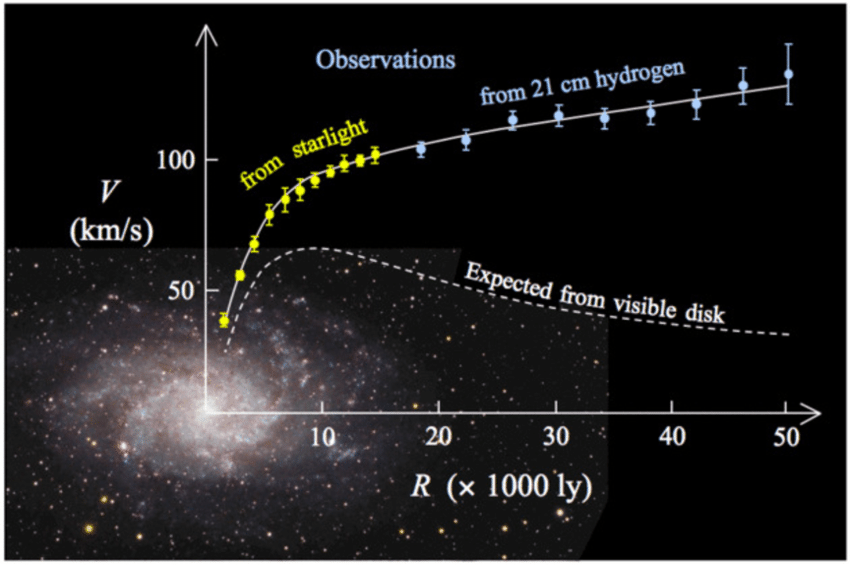
\includegraphics[width=0.75\textwidth]{figures/chapter_DM/M33-rotation-curve}
        \caption{
            Figure here shows the galactic rotational curve of M33, the expected rotational curve is shown in the dotted line. Experimental evidence observes behavior in the solid line.~\cite{M33}.
        }
        \label{fig:M33_figure}
    \end{center}
\end{figure}


\subsection{Gravitational Lensing}

    General relativity shows that massive objects would curve the space-time curvature around them. The details are capulated elegantly in the Einstein's Equation: 
%~\ref{eq:Einstein}: 

\begin{equation}
	R_{\mu \nu} - {1 \over 2}R \, g_{\mu \nu} + \Lambda g_{\mu \nu}= {8 \pi G \over c^4} T_{\mu \nu}, 
    \label{eq:Einstein}
\end{equation}

	In this equation, $R_{\mu \nu}$ is the Ricci curvature tensor, and R is the scalar curvature, together they form the Einstein tensor. $g_{\mu \nu}$ is the metric tensor, and $T_{\mu \nu}$ is the stress-energy tensor. This equation shows that the curvature of space-time is directly related to the mass and energy in that space. 	
	
	Consequentially, light rays that travel through the curved space-time around the massive object would therefore be bent. The effect mirrors that of angled lenses bending light rays due to a velocity difference of light rays across different media, and is called gravitational lensing. 

	There are different forms of lensing effect, roughly arranged by the strength of their effects. Strong lensing effect happens when bending of light result in either multiple images, a light ring or an arc, more typically observed around massive centers of galaxy clusters and galaxies; weak lensing usually involves statistical analysis of many objects over a large region; micro-lensing is detected when the effect only displays as an apparent change in the brightness of the source.

    Figure~\ref{fig:BulletCluster_figure} shows the bullet cluster collision of 1E 0657 -56. It is produced from the combination of gravitational lensing and x ray telescope imaging. The red part of the diagram denotes ordinary matter and the blue part reflects dark matter. In the cluster collision, ordinary matter bend light around them and became luminous from the collision, captured by x-ray imaging; the blue part shows a part of the clusters that did not interact and light up in the collision via gravitational lensing. This is a strong evidence for the existence of non-luminous matter in the clusters.

\begin{figure}[!htb]
    \begin{center}
        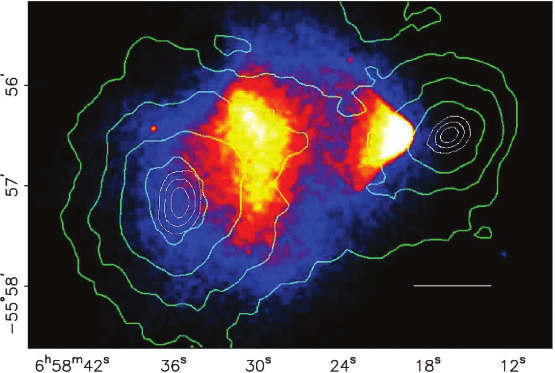
\includegraphics[width=0.75\textwidth]{figures/chapter_DM/BulletCluster}
        \caption{
			Bullet cluster (1E 0657-56) showing two colliding galaxy clusters, the part in red came from x-ray image by Chandra, highlighting normal matter distribution; the part in blue came from gravitational lensing. ~\cite{BulletCluster}.
        }
        \label{fig:BulletCluster_figure}
    \end{center}
\end{figure}


\subsection{Cosmic Microwave Background}

    In the beginning of the universe, ordinary matter and dark matter all exist in a hot plasma soup with frequent interaction between charged particles and photons through Thomson scattering. There comes a very important period in the universe called the recombination period, where the expansion of the universe has cool the plasma soup enough that charged particles began to form neutral atoms. Photons stopped scattering on the charged particles and went on unhindered. Due to red
shifting effect, they form a microwave background of the universe that can still be observed today. This is the Comic Microwave Background. 
This original background is nearly a black body and is therefore very uniform, but there exists small temperature variations. The variation can be decomposed into an angular power spectrum, as shown in Figure~\ref{fig:CMB_figure}

Due to the different interaction between dark matter and ordinary matter with photon and each other, simulation shows that different dark matter and ordinary matter make-up of the universe would result in different angular spectroscopy shape. 

Study from Planck on cosmic microwave background Figure~refgives a clear composition and percentage abundance of dark matter. Dark matter is not only an essential part of the universe, its composition is approximately 5 times as large as ordinary matter. Giving evidence that dark matter makes up the majority of the universe. 
%\figure planck 

\begin{figure}[!htb]
    \begin{center}
        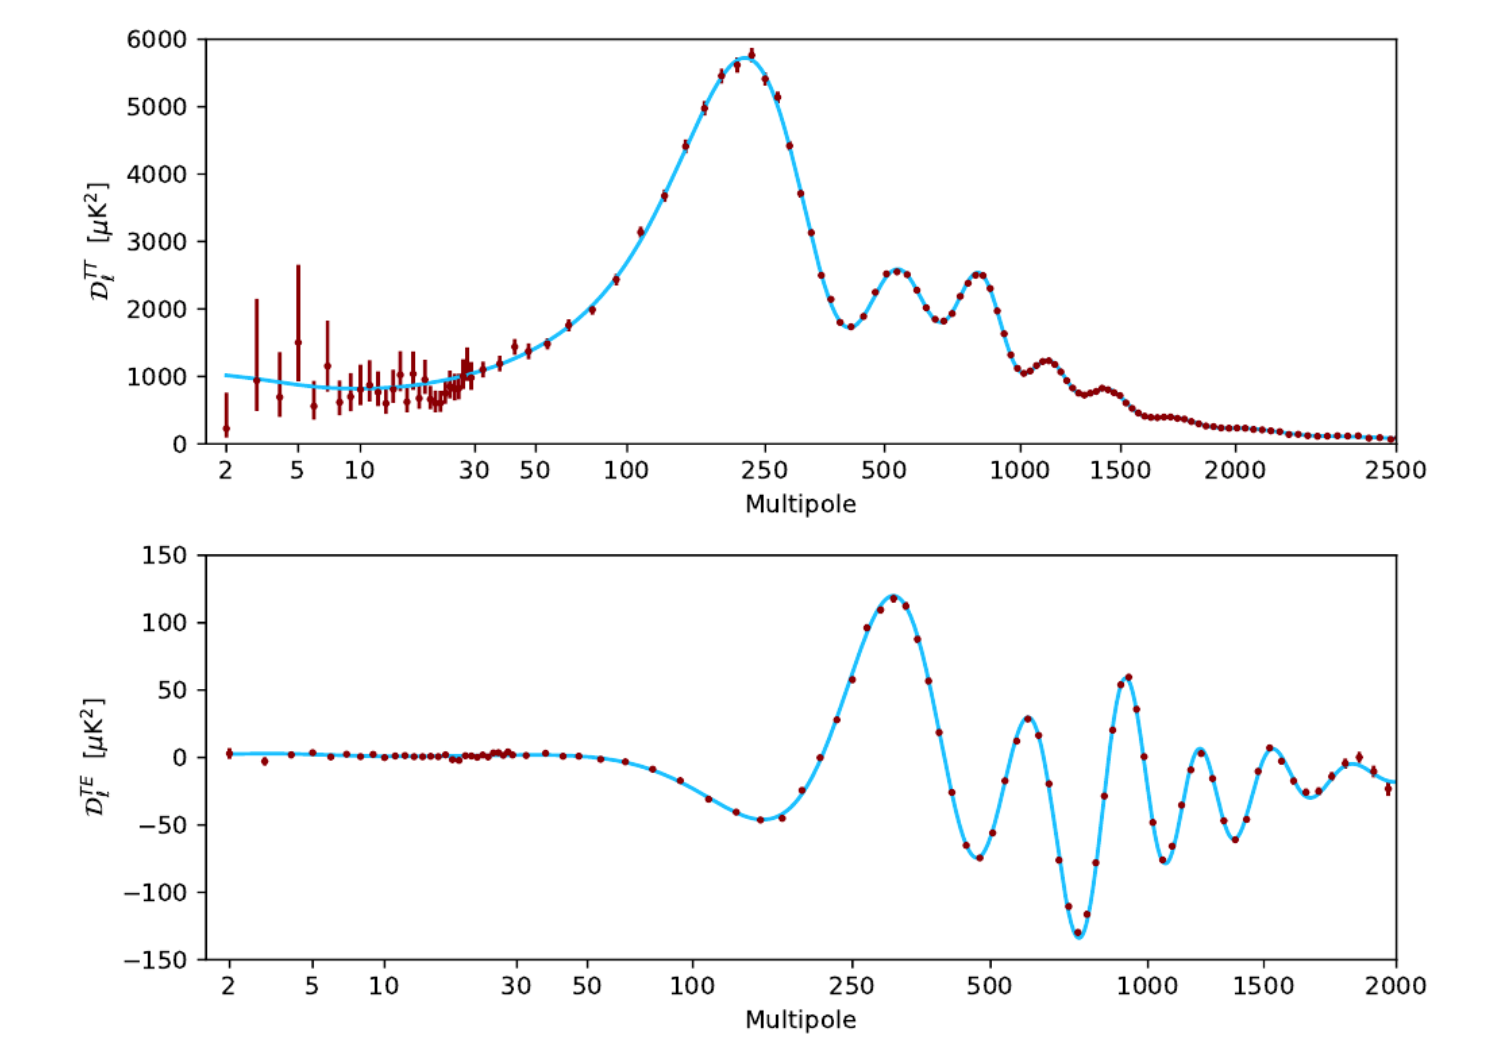
\includegraphics[width=0.75\textwidth]{figures/chapter_DM/CMB-angular-power-spectrum}
        \caption{
			The Cosmic Microwave Background power spectrum measured by Planck.~\cite{CMB}.
        }
        \label{fig:CMB_figure}
    \end{center}
\end{figure}


%\subsection{Large Scale Universe Structure}
%Gravity has a deterministic effect on how the universe is formed, and therefore affects the large scale structure of the universe. The existence of dark matter 
%https://www.forbes.com/sites/startswithabang/2020/10/02/ask-ethan-can-dark-matter-really-explain-the-universes-structure/?sh=5b37659b3b06


\section{Properties}
\label{section:properties}
While dark matter itself has never been directly observed, many studies in the cosmological, astrophysical and particle scale has constrained much of its properties. In this section and the remaining thesis, the following properties of dark matter will be assumed along with its justifications.

\subsection{Dark}

Dark matter got its name from its little to no interaction with light compared to ordinary matter in cosmological observation. Collision of the bullet cluster has also greatly constrained its interaction with itself.  
It is taken that it will not interact with collider detector and its interaction with ordinary matter would be rare in the energy scale of the LHC. 

\subsection{Long Life Time}

As dark matter is seen today in evidence across difference scales (see section ~\ref{section:evidence}). It is assumed to have a long life time since its creation in the early universe. Many theoretical model of dark matter require a $Z_{2}$ symmetry (such as the R parity of supersymmetry). This prevent dark matter particles from decaying into lighter Standard Model objects. In most experimental searches today, it is be treated as a single particle that does not decay further into other detectable SM particles. ~\cite{boveia2018dark}


\subsection{Interact Gravitationally}
Current evidence (see section ~\ref{section:evidence}) suggests that dark matter is massive (i.e. it interacts gravitationally). However, there is no consensus on the mass on the individual parts of dark matter. Current theoretical candidates of dark matter roughly be split into two camps: cold dark matter and hot dark matter. The former group believes that dark matter is made of object massive enough to be non-relativistic; the latter group hold the opposite view. 

\subsection{Cold}
In cosmology, hot/cold refers to the mass of an object. Only objects relatively low in mass would be affected relativistically. Different assumption of the relativistic mass of dark matter has great impact on the galaxy formations and its distribution. From most simulation results, dark matter is taken to be non-relativistic by most physicists and will be assumed for dark matter candidate searched for in the rest of the thesis. 

\subsection{Low Self-Interaction}
Dark matter is believe to have little to no self interaction, Mixed X-ray, optical and gravitational lensing study on the merging galacy cluster 1E-657-65 has restricted its self interaction limit to below $\sigma \over m < 1.25 cm^{2} g^{-1}$ (68\% confidence)~\cite{randall2008constraints}. 
 
%\subsection{Single Particle}
%While there are many composite dark matter models being proposed these days, dark matter is still taken to be a single kind in most effective model/simplified model building for experimental searches. 

\section{Candidates}
\label{section:candidates}

There exist a wide range of candidates for what dark matter could be. In here, a few possible particle candidate of dark matter are outlined here. 

\subsection{Sterile Neutrino}
Standard model does not predict that neutrino has a mass, however, that contradicting with experimental finding and is therefore a problem of the standard model. By replacing right-handed neutrinos in the standard model with gauge singlet fermions that has no interaction other than mixing with normal neutrinos, sterile neutrino is formed by theoretical models. Tuning parameters such its interaction rate with normal neutrino, mass and mixing angle, sterile neutrino can be a possible candidate for dark matter, as it can lead to a right
density of dark matter with stability consistent with the scale of the universe. ~\cite{dodelson1994sterile} They are searched for in radiator experiments such as the Daya Bay \cite{an2014search, wong2017search} and in scintillator experiments like DANSS. ~\cite{alekseev2018search}

% Mass and range  mass keV scale, currently sterile neutrino mass is unknown and therefore can be either hot or cold

%Daya Bay Collaboration, F. P. An et al., “Search for a Light Sterile Neutrino at Daya Bay,” Phys. Rev. Lett. 113 (2014) 141802, arXiv:1407.7259 [hep-ex].
%1310.8642
\subsection{Axion}
Another exisitng problem in the standard model is the strong CP problem. The strong CP problem points to the unnaturalness of CP symmetry observed in neutrons charge distribution measurement. This gives an exceptionally small value to the term that govern strong CP violation in the Standard Model, which is unnatural. The problem can be solved by introducing an additional axion particle and its associated fields to the standard model. ~\cite{peccei1977cp} With the proposition of such field, the CP violation term in strong interaction will be cancelled out naturally, thereby giving an explanation to the unnaturalness to the experimental value. 
The axion proposed is a dark matter candidate, as its calculated life time is much greater than the age of the universe and it shares many properties with the known profile of dark matter. Recent experimental finding from the XENON1T and shows anomalies that could be signs of axions. ~\cite{aprile2020excess}
%ADMX mass mu eV
%https://arxiv.org/pdf/2105.01406.pdf

%Xenon Collaboration, E. Aprile et al,. "Excess Electronic Recoil Events in XENON1T", Phys. Rev. D 102, 072004 (2020), arXiv: 2006.09721


% Non-particle candidates
%\subsection{Modified Newtonian Gravity}
%\subsection{MACHOs}

\subsection{Weakly Interacting Massive Particle (WIMP)}
A very attractive candidate for dark matter is called the weakly interacting massive particle(WIMP). It appears naturally with many Beyond-the-Standard-Model theories that aim to solve other physics problems, including theories of supersymmetry with R-parity and some extra dimensional theory. 
In the study of dark matter in cosmology, it is frequently assumed to be a thermal relic. Thermal relic dark matter is in thermal equilibrium with ordinary matter in the early universe. In thermal equilibrium with ordinary matter, it gets produced and annihilated at the same rate. There comes a point in the universe called freezing out, where the expansion of the universe cools the particle bath and produce temperature lower than possible to produce enough energy statistically for dark matter to
be produced given certain dark matter mass. Dark matter production from ordinary matter ceased. As the universe further expanse, it becomes more difficult for dark matter to find each other to be annihilated to form ordinary matter. Dark matter abundance is locked at this point and remained unchange until today. 
Using this model and the current measured abundance of dark matter in our current universe, the self annihilation cross section of dark matter is $ \langle \sigma \cdot v \rangle \simequal 3 \cdot 10^{26}cm^{3} s^{-1}$. This annihilation cross section scale matches many prediction made in supersymmetry theories. Many Beyond-the-Standard-Model theories, such as SUSY, the Universal Extra Dimension Model, and the little Higgs all predict a particle with known dark matter properties and self interaction rate of the same scale. This is known as the WIMP miracle. ~\cite{Dev_2014}

%\Figure WIMP miracle


\begin{figure}[!htb]
    \begin{center}
        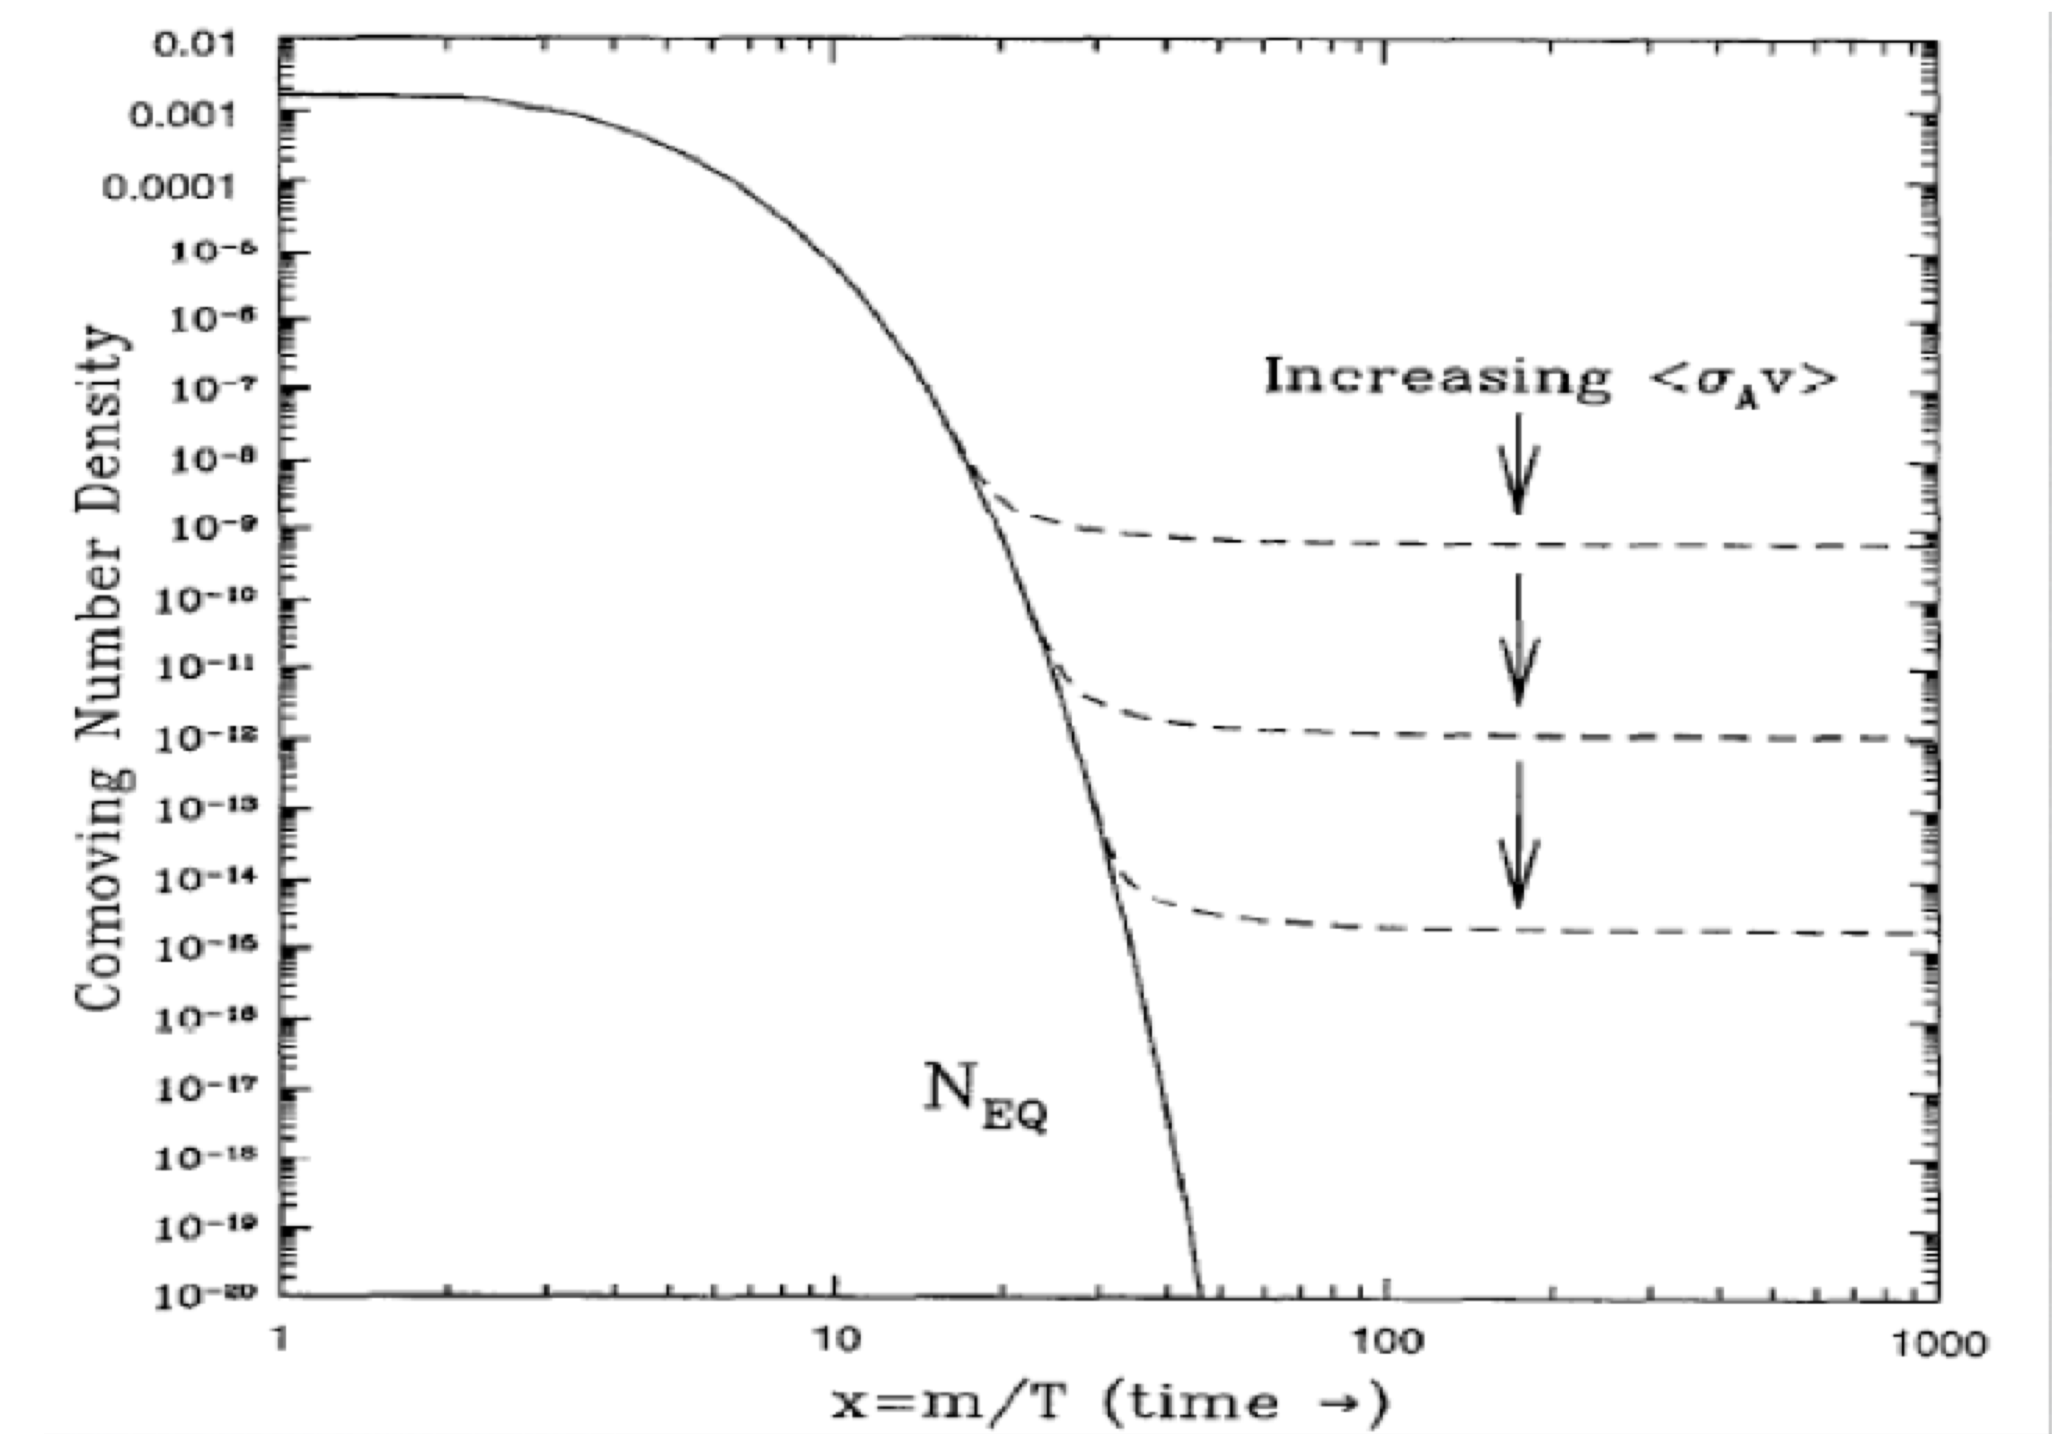
\includegraphics[width=0.75\textwidth]{figures/chapter_DM/WIMP}
        \caption{
		Solid line here shows the change in the densitiy of dark matter in an expanding unverse. In the early universe, the solid line is horizontal, indicating the time when dark matter production and annihilation is equal. The line gradually fall with increase of time when production rate began to decrease with the universe expansion. Later as the universe further expands, the annihilation stops as well and dark matter gets freezes out to different density level with different assumed self interaction annihilation rates.~\cite{WIMP}.
        }
        \label{fig:WIMP_figure}
    \end{center}
\end{figure}


 

%P.S. BHUPAL DEV, ANUPAM MAZUMDAR, & SALEH QUTUB, FRONT.IN PHYS. 2 (2014) 26
%https://indico.cern.ch/event/473000/contributions/1993414/attachments/1209863/1764345/tait-Aspen.pdf

%https://www.particlebites.com/?p=7004
%https://www.forbes.com/sites/startswithabang/2019/02/22/the-wimp-miracle-is-dead-as-dark-matter-experiments-come-up-empty-again/?sh=5ebc59f46dbc

\section{Experimental Search Overview}
\label{section:searches}

Traditionally the search for dark matter is split into different experimental categories sorted by the different detection methods from different dark matter/normal matter interactions. 

\begin{figure}[!htb]
    \begin{center}
        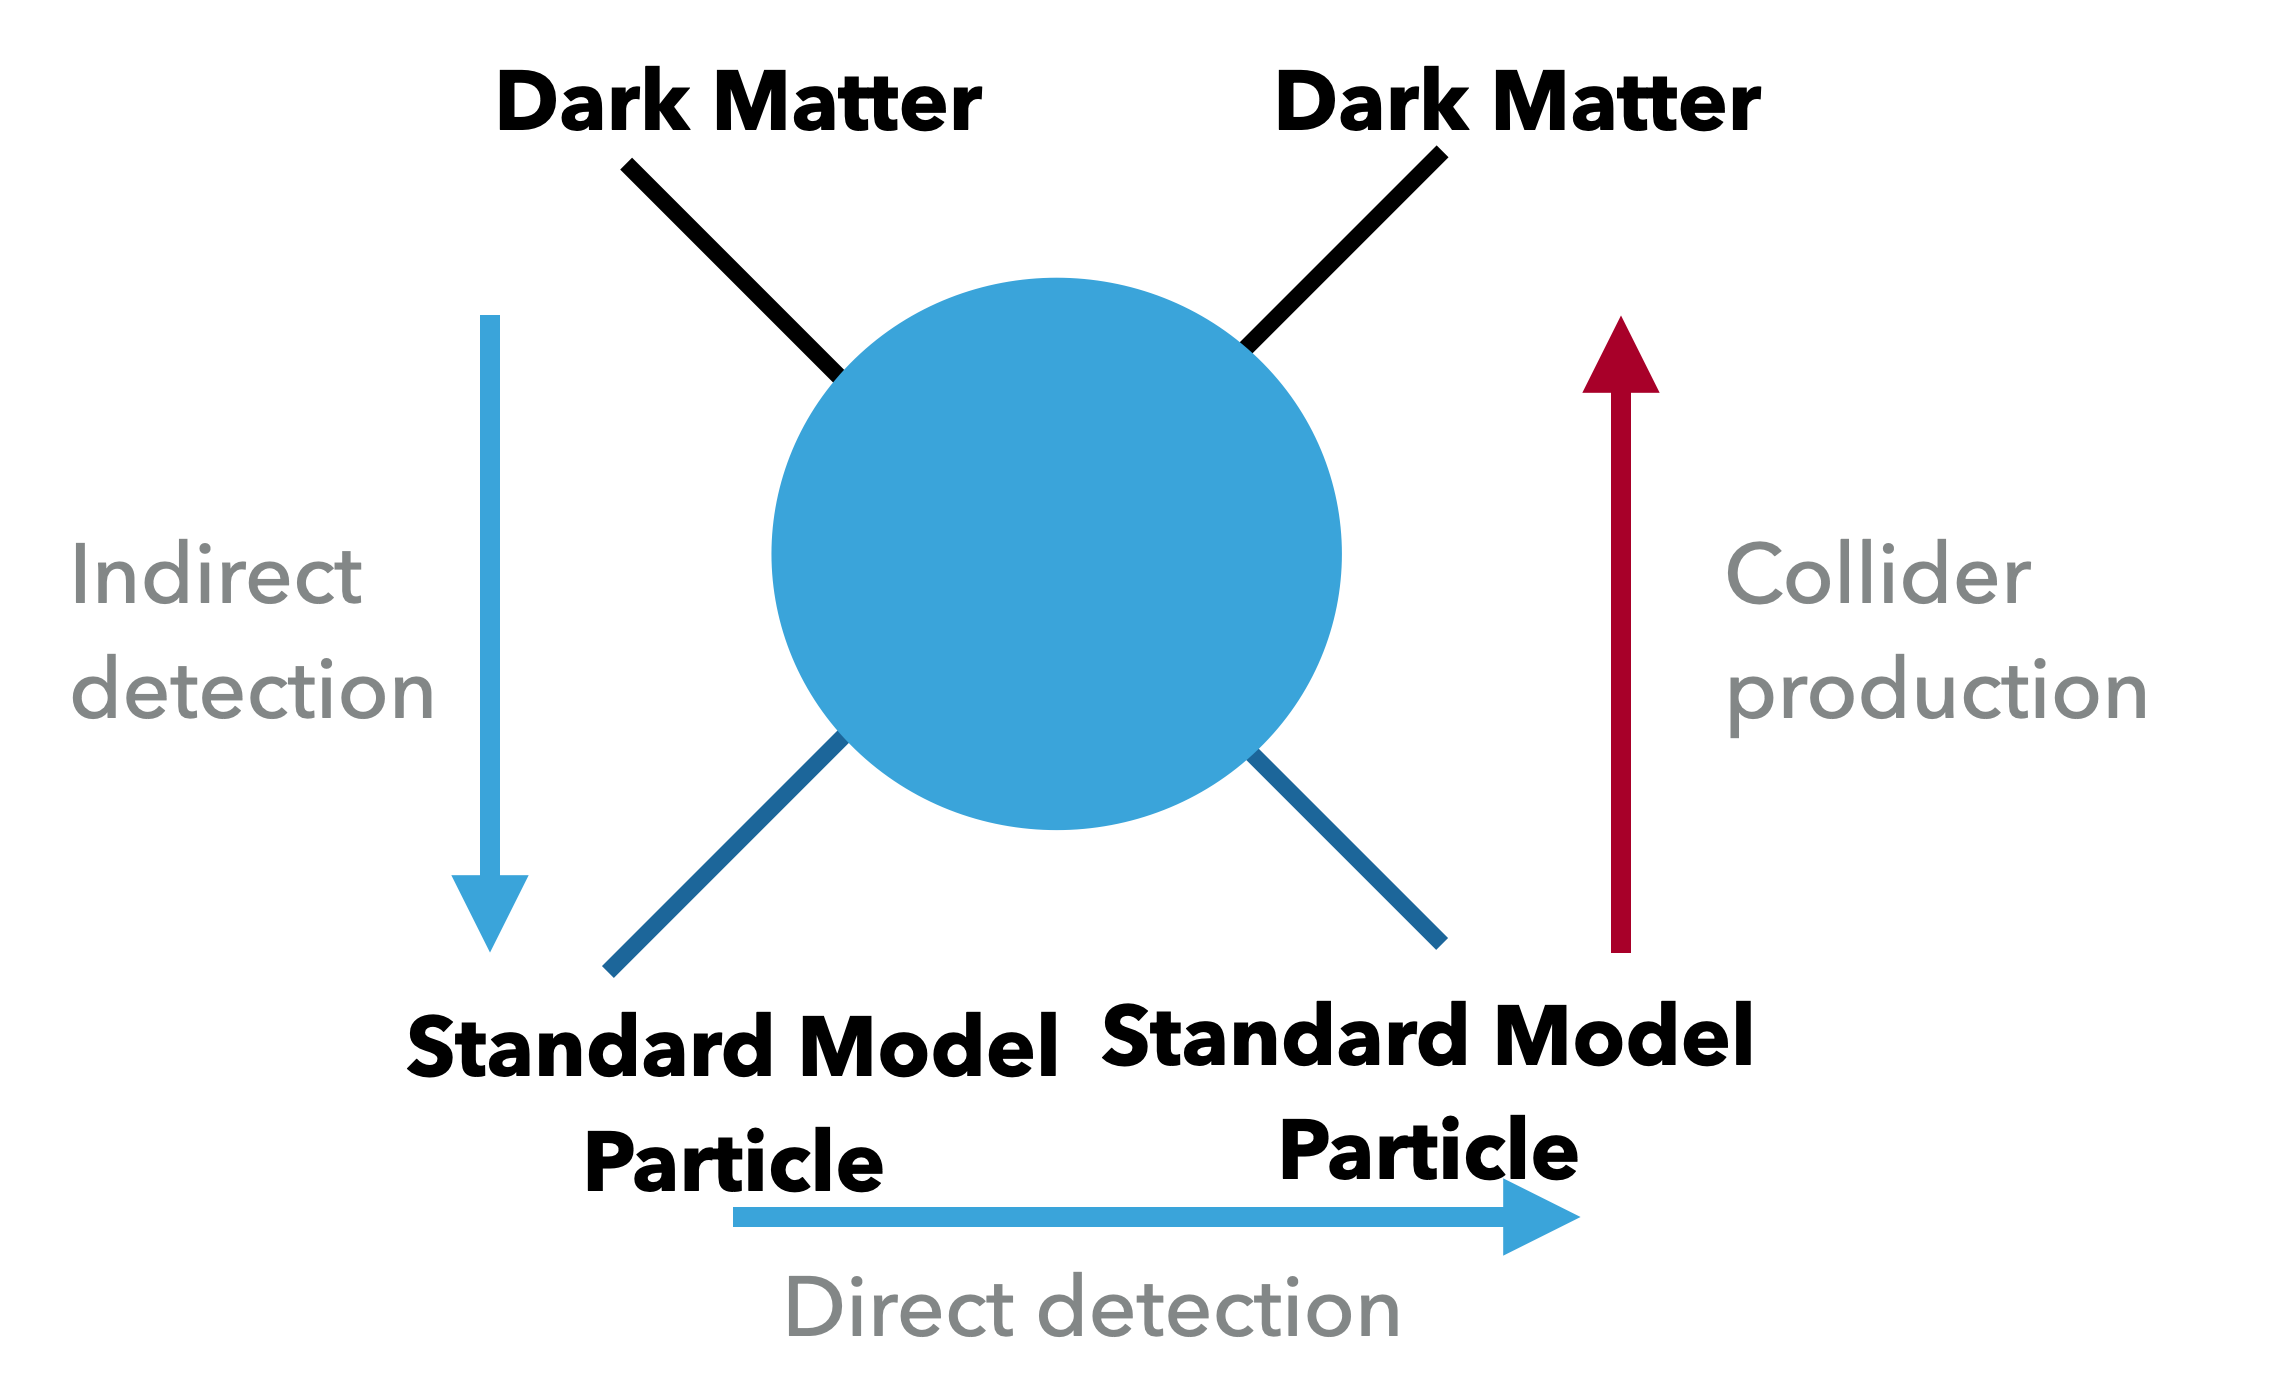
\includegraphics[width=0.75\textwidth]{figures/chapter_DM/Interaction}
        \caption{
			Schematic cartoon showing the different dark matter detection methods facilitated by different interactions thus signatures. 
        }
        \label{fig:interaction}
    \end{center}
\end{figure}

\subsection{Direct Detection}
Dark matter is believed to travel through the universe and passes through the eath. Assuming weak interaction between dark matter and Standard Model nucleons, dark matter can be detected directly with different target objects. 

\[ R \propto N \rho \chi \langle \sigma_{\chi } N \rangle \]

There are different experiments that uses different material and targets different dark matter masses.
Notable experiments include LZ ~\cite{mckinsey2016lz},   Xenon1T ~\cite{aprile2020excess}, SuperCDMS ~\cite{Agnese_2016}, CRESST ~\cite{Angloher_2014} and DAMA ~\cite{Bernabei_2008}. 

As more experiments has excluded much of the theory model phasespace, many of the experiments now faces the challenge of the neutrino floor in low mass dark matter search, which is where neutrino background began to dominate signal region. 



\subsection{Indirect Detection}
Indirect detection looks for annihilation Standard Model product of dark matter. It looks for interaction in places where matter is dense enough to interact, usually in center of galaxies and stars. Experiments include FermiLAT ~\cite{albert2017searching} and H.E.S.S. ~\cite{aharonian2006hess}


\subsection{Collider Production} 
    In the Large Hadron Collider, dark matter can be studied by being directly produced from Standard Model particles.

\section{Theoretical Models in LHC Searches}
\label{section:models}

While there exist a wide range of speculation on the identity of dark matter, the use of LHC as a dark matter searching tool constrains a unique set of dark matter candidate accessible phenomenologically. 
Focusing phenomenologically observable and interpretability for a wide range of theoretical models, different modeling approaches are used to develop benchmark models searching for dark matter in the LHC.
Sorting by an ascending degree of completeness, the literature will review different approaches and models of dark matter used in the LHC.


\begin{figure}[!htb]
    \begin{center}
        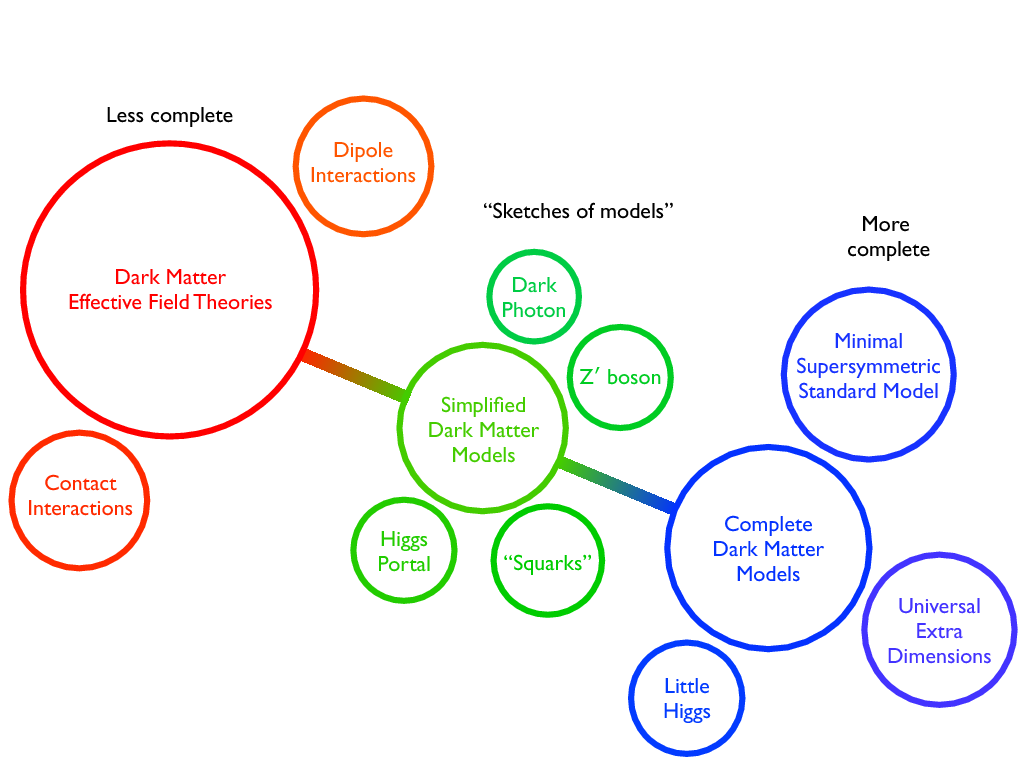
\includegraphics[width=0.75\textwidth]{figures/chapter_DM/Model}
        \caption{
			Colored Scheme showing dark matter modeling approach from more simplistic (left) to more complete models (right).  ~\cite{Abdallah:2024101}.
        }
        \label{fig:Model_figure}
    \end{center}
\end{figure}



\subsection{Simple Portal Models}
The simplest kind of models are simple extensions to the standard model. In these models, dark matter is mediated either through the Higgs or the Z Boson. As the Z portal models are constrained by LEP and DD experiments, dark matter that are mediated through a heavier version of Z boson ( the Z') and additional scalar is also searched for. 

\subsection{Effective Field Theory}
The effective field theory approach condenses a wide range of complete models to simplified versions by focusing on what is experimentally accessible. High mass mediator particles in complete theories as a contact operator. High energy correction and details are integrated out for "effectiveness". All kinematically accessible observables are described by a Lorentz structure and a rate parameter. 
This approach allow for the easily measured experiment values and a framework for a wide range of complete models to be probe with few experimental model search. However, the model has a singularity and is not valid for when the interaction momentum transfer is close to that of the mediator mass. In the LHC, a truncation method is used to bound the events simulated Monte Carlo events below this limit ~\cite{Busoni_2014}.

\subsection{Simplified Model}
The problem in effective field theory can be resolved with the simplified Model appraoch. The contact interaction in EFT is turned into mediator particle s-channel/t-channel exchanges in simplified model. With the price of an increased number of parameters, simplified models can provide the full mechanics of a particle interaction and usually come with more details. 
Simplified models of dark matter in the LHC do not break the global and gauge symmetries of Standard Model, the Lagrangian terms are Lorentz invariant and predicts at least a dark matter candidate that fullfills the properties described in the previous section. 
Some simplified dark matter model used in the LHC include the Two-Higgs Doublet Model (2HDM), where Higgs or a non-standard model exotic Higgs could serve as a mediator to dark matter; other examples include dark photon or a kinetically mixed Z' dark matter model. 
Other than these, simplified model in supersymmetry such as the Phenomenological Minimal Supersymmetric Standard Model (pMSSM) which reduces the over 100 parameters of complete model of Minimal Supersymmetric Standard Model to 19 parameters, predicts candidate dark matter like particles, predicts neutralino as a natural dark matter candidate. 
In addition, other gauge or gravity mediated SUSY theory predicts gravitino as a dark matter candidate. 
% pMSSM Assumes no sources of CP violation Beyond-the-Standard-Model and no flavor-changing neutral currents, and retains uni- versal couplings and masses for first- and second-generation superpartners. %CatDog Antonio DM summary paper.  

\subsection{Less-simplified models}
The LHC dark matter working group is moving towards less simple models with more phenomenological details.
%\subsection{Long-Lived Particle Models}

A detailed list of models used by the LHC by both the CMS and ATLAS can be found in this reference ~\cite{Abercrombie_2020}.

\subsection{The LHC Dark Matter Benchmark}
\label{sec:LHCDM}
The dark matter benchmark from the LHC uses the effective field theory approach. (See section for more detail on this appraoch) It uses contact interaction operator as the basis of the theory model building blocks. This way, the model can be reduced to a handful of experimentally measurable qualities for more complete theory model interpretations. 
In the dark matter benchmark of the LHC, it extends the Standard Model by an additional U(1) symmetry, and assumed dark matter along with some Stanard Model particles are all charged under this. A new gauge boson can thereby facilitate interaction between the standard model and dark matter field. 

The dark matter mediator can either be an axial vector or a vector, the corresponding lagrangians are as such:

\[ \mathcal{L}_{vector}= g_{q} \sum$_{q=u,d,s,c,b,t}$ Z'_{\mu}\bar{q}\gamma^{\mu}q + g_{\chi}Z'_{\mu}\bar{\chi}\gamma^{\mu}\chi \]


\[ \mathcal{L}_{axial vector}= g_{q} \sum$_{q=u,d,s,c,b,t}$ Z'_{\mu}\bar{q}\gamma^{\mu}\gamma^{5}q + g_{\chi}Z'_{\mu}\bar{\chi}\gamma^{\mu}\gamma^{5}\chi \]

This is also applicable to leptons, under this calculation the minimal parameters of the model is reduced to {g_{q}, g_{\chi}, m_{\chi}, M_{med}}. 

Similar arguments can be made for the lepton couplings. 

On ATLAS, these models are generated in the event generator with NLO+PS accuracy with the POWHEG generator, the product goes through parton showering at PYTHIA8 with detector simulation from GEANT4. 


\section{Experimental Signature in the LHC}
\label{section:signatures}

\subsection{Mono-X signature}
    This describes the type of dark matter search where an invisible dark matter is produced directly in the LHC and is "observed" in the detector as missing transverse momentum.
    Dark matter is known to interact only very weakly with normal matter, and thus is assumed to not leave a trace in the LHC detector. When events are produced through proton-proton collision along the z-axis in the LHC, the momentum of all objects along the transverse plane to the z-axis is always zero. Therefore, when an event has missing transverse momentum recoiling against another visible object, the signature would possibly be dark matter.
This class of analysis is named by the standard model object that dark matter recoil against. Mono-jet, mono-Higgs, mono-Z are a few analyses done this way. 

\subsection{Di-object Signature}
    Dark matter can also be searched for without the production of the dark matter particle. The simplified models that predicts dark matter in the mono-X analyses predicts effective mediator particle between standard model particle with dark matter. These effective mediator particles can be directly searched for through via decay back into standard model object. As the process is distinct from any known Standard Model particle processes, an excess of events Beyond-the-Standard-Model prediction for
    such a mediator process could be evidence for dark matter in the LHC. 
These di-object search include dijet, dilepton, diphoton searches. 
In recent years, new techniques such as the trigger-level-analysis and channels that has an additional initial state radiation objects are being pioneered. These result in a search phasespace much greater than the traditional program and greatly extended the of the richness of the LHC serach program.

\subsection{Supersymmetric Signature}	

\subsection{Long-Lived Particle Signature}


The Signature used for this analysis 

\chapter{The Large Hadron Collider And the ATLAS Detector}
\label{chapter:ATLAS}

All data used in this thesis is taken from the ATLAS experiment~\cite{ATLAS:1999vwa} of the Large Hadron Collider(LHC)~\cite{Bruning:782076} in the European Organization of Particle Physics(CERN).

CERN is the largest research organization on particle physics in the world. (See Figure~\ref{fig:LHCOnBorder}for a schematic map) The laboratory was built in the 1950s as a joint European effort to advance particle physics. It includes a total of 23 member states to date. Many major physics discoveries were made at CERN. Most notably, the discovery of the W, the Z boson~\cite{hioki1982does}, and the first man-made antihydrogen atom~\cite{hioki1982does}. In 2012, a boson of mass 125 $GeV/c^{2}$ was discovered, it is believed that it matches the
profile of the long sought after Higgs Boson particle~\cite{chatrchyan2012observation}, which gives an explanation to the origin of mass of matter in the universe. The site with 2660 on-site personnels and 12,400 users from over 70 countries also produced many technological derivatives outside of scientific discoveries. In particular, the World Wide Web was first built at CERN~\cite{berners1994world}.

This chapter presents the hardware and software apparatus in the LHC at CERN used to collect and produce the datasets for the later analyses.
The working and the layout of the LHC, the machine used to accelerate protons and monitor its collisions is presented in Section~\ref{LHC}; the ATLAS detector, the apparatus used to collect proton-proton collision data is described in Section~\ref{ATLAS}. Lastly, the triggering chain: the hardware and software collecting strategy is presented in Section~\ref{trigger}.

\begin{figure}[!htb]
    \begin{center}
        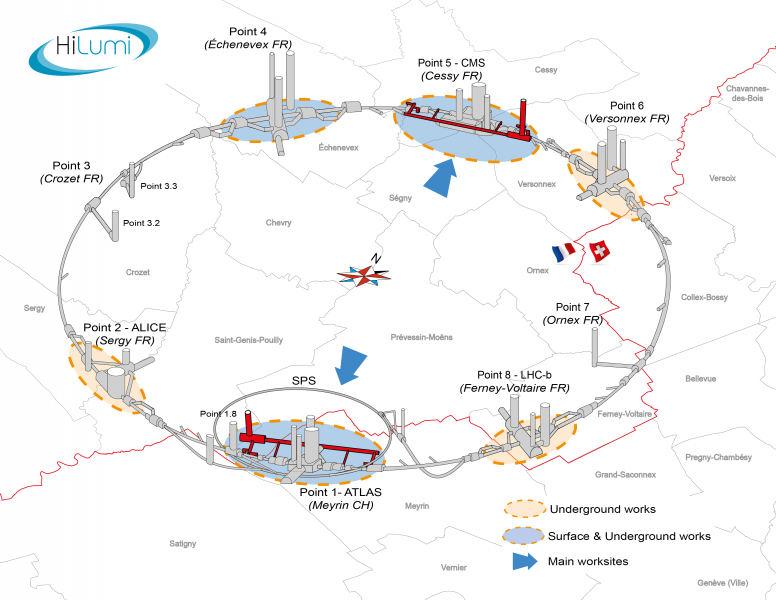
\includegraphics[width=0.75\textwidth]{figures/chapter_ATLAS/LHCOnBorder}
        \caption{
            This figure shows where the CERN is located geographically, across the border between France and Switzerland~\cite{Bruning:782076}.
        }
        \label{fig:LHCOnBorder}
    \end{center}
\end{figure}

\section{The Large Hadron Collider}
\label{LHC}

The LHC is located on the France-Switzerland border. Its main ring is a 27 kilometers tunnel that is 175 meters underground. It's mainly used to collide protons. Lead-lead collisions and proton-lead collisions are also done for a few weeks in each data-taking year. 

The collider was a planned successor to the Large Electron-Positron (LEP)(209 GeV collision) and the Tevatron collider (1TeV) in Fermilab. Since the last two experiments, the community converged on a consensus of an O(10)TeV scale proton collider with the main physics goal to probe electro-weak scale Higgs boson, beyond-the-Standard-Model physics, and further Standard Model measurement studies. The LHC was born.

The LHC reuses the same tunnel as the LEP experiment, with some major modifications were done to the tunnel for the upgrade: to achieve higher center-of-mass energy and to collide proton-proton instead of electron-positron, the angular velocity of the particle colliding would need to be raised. The existing magnet from the LEP experiment was therefore replaced to make way for more powerful cryogenic-based super-conducting magnets to bend higher speed particles. In addition, as the LHC uses a proton-proton beam rather than an electron position in the LEP, an extra beam pipe was required. This is due to the fact that the proton beams collisions could not share the same beam pipe as the position-electron beams in the LEP. The radio frequency system is also modified in the upgrade to the LHC to allow for acceleration of the two separate beams in the LHC.

After the upgrade, the main ring of the LHC allows for particle collision to happen in four main intersection points. These four points are directly inside the four major experiments of ATLAS~\cite{ATLAS:1999vwa}, CMS~\cite{CMS:2006myw}, LHCb~\cite{lhcb2001technical} and ALICE~\cite{Cortese:519145}: 

ATLAS and CMS are general-purpose detectors, data collected from these experiments are used for studies including Standard Model measurement, Higgs property measurement as well as exotic and new physics searches. The similar but slightly different detector structure between the two experiment allow for crosschecks and validation of physics results. ALICE is optimized to study strong physics in the quark-gluon plasma generated from lead-lead collisions. LHCb is a forward detector that specializes in b(bottom quark)-physics measurement. Studies on the bottom quark done in LHCb measures CP violation parameter and could help better understand matter-antimatter asymmetry of the universe. 

In addition to the four major experiments, the LHC currently hosts four more experiments. LHCf looks for forward particles that originate from cosmic radiation~\cite{Adriani:926196}. FASER is an experiment in search of long-lived exotic particles with a lifetime beyond the ATLAS detector~\cite{Ariga:2651328}. MoEDAL, which sits in the cavern of LHCb, looks for the magnetic monopole or highly ionizing stable massive particles (SMP)~\cite{Pinfold:1181486}. TOTEM shares the CMS interaction point; it measures the total
cross-section, diffraction process and elastic scattering processes of particles in the proton collisions~\cite{TOTEM:2004hps}. 

The LHC is designed to operate at a maximum center-of-mass energy of 14 TeV. Protons that get collided at the different interaction points go through many stages before collisions. 

In the following sections, some technical terms related to LHC operation will be discussed. Different parts of the LHC from proton production, proton acceleration to proton collision in the center of the ATLAS detector is also covered.

\begin{figure}[!htb]
    \begin{center}
        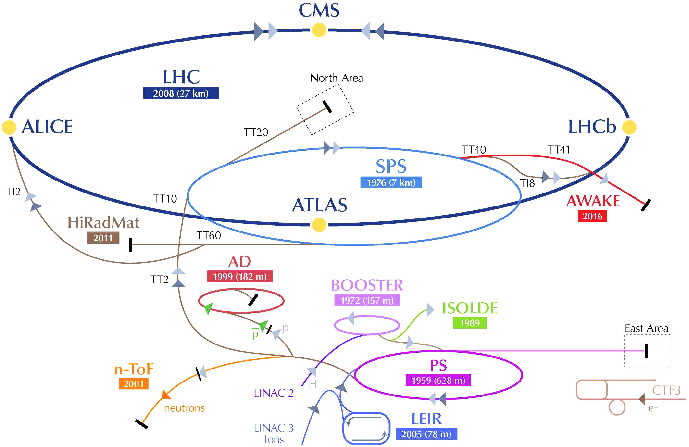
\includegraphics[width=0.75\textwidth]{figures/chapter_ATLAS/LHCAcceleratorComplex}
        \caption{
			This figure shows the accelerator complex of CERN, featuring the experiments and injection chain of the LHC~\cite{Marcastel:1621583}.
        }
        \label{fig:CERNAcceleratorComplex}
    \end{center}
\end{figure}

\subsection{Luminosity}
The instantaneous luminosity is a measure of how many events can be produced under certain detector conditions. It's directly related to the event rate of different processes under production.   
The quantity is given as the following:

\begin{equation}
    L = \frac{F \cdot N^{2}_{p} n_{b} f_{\lambda}}{4\pi\epsilon \beta^{*}}
\end{equation}


\begin{equation}
    \rightarrow = \frac{N_{\textrm{proton in beam 1}} \cdot N_{\textrm{proton in beam 2}} \cdot \textrm{Beam Crossing frequency }}{\textrm{Beam overlap Area}}
\end{equation}

In the formula above, $N_p$ is the number of proton in each beam, $n_{b}$ is the number of bunches per beam, f is the frequency of the beam traveling around the collider, and $\beta^{\*}$ is the beam cross-sectional size at the injection, $\epsilon$ is the beam emittance, F is the beam crossing angle.

The LHC was built to have a peak luminosity at L=$2 \cdot 10^{34}cm^{-2}s^{-1}$, but in most of Run II, it has a nominal value of $10^{34}cm^{-2}s^{-1}$.

While the instantaneous luminosity is a measure of LHC performance in operation, integrated luminosity, denoted by $\mathcal{L} = \int L dt$ is a measure of the amount of data taken over time.

While an increase in instantaneous luminosity increases the event rate in the experiment, it also increases the pile-up, which is multiple occurrences of interactions that happened simultaneously as the target events. Pile-up cleaning will therefore become an increasingly important task as the LHC instantaneous luminosity goes up.

\subsection{Proton Production}
The protons that collide in the LHC came from hydrogen in gaseous form. The electrons are stripped out from getting sent through an ion source. Protons formed are grated to make sure they are in the same direction before being sent off to the injection chain for acceleration. 

\subsection{The Injection Chain}
The acceleration of protons after their production is done through the so-called injection chain. It mainly consists of a series of pre-acceleration steps through the different linear booster and booster rings. As the speed and energy of the particle are effectively restricted by both the accelerator ring size as well as magnet strength in a cyclotron accelerator, a dedicated series of smaller rings in ascending order in size are used to accelerate the beam to a higher energy level before the LHC ring.

The protons first go through a linear accelerator named LINAC2 to be accelerated to 50 MeV. After the acceleration, they enter a synchrotron ring called the Proton Synchrotron Booster, the protons are accelerated to 1.4 GeV at this stage. Subsequently, they are injected into the Proton Synchrotron(PS). The PS accelerates the protons further to 26 GeV and is injected into the Super Proton Synchrotron(SPS), the protons are then further accelerated to 450 GEV and passed onto the LHC ring in \textit{proton bunches}.

These booster rings are existing structures from previous collider experiments~\cite{ATLAS:1999vwa}.

\begin{figure}[!htb]
    \begin{center}
        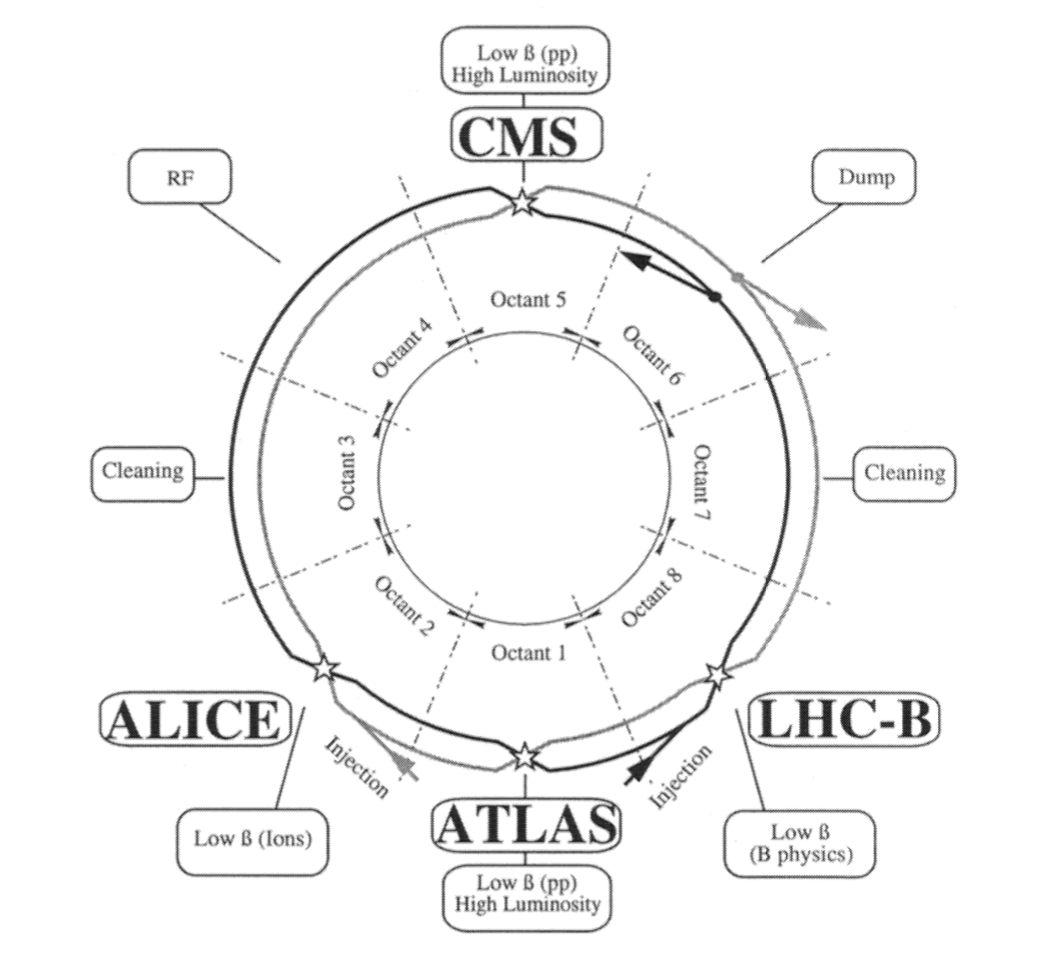
\includegraphics[width=0.75\textwidth]{figures/chapter_ATLAS/LHCRing}
        \caption{
			This figure shows the different parts of the two LHC rings along with its features~\cite{Pettersson:291782}.
        }
        \label{fig:perterson}
    \end{center}
\end{figure}

\subsection{The Radio Frequency Cavities}
After the injection to the LHC, the protons will be further ramped up in energy. Located in IP4 of the LHC main ring, the radio frequency(RF) cavity of the LHC performs the acceleration of particles in the ring. The cavity oscillates its electric field at a fixed 400MHz rate, which accelerates the incoming well-timed protons. In Run II, Protons that arrive in the LHC are accelerated from the 450 GeV injection energy to 6.5 TeV in 10 million loops around the LHC, which takes approximately 20 minutes. Other
than accelerating protons, the cavity also modulates the protons' energy: the slowed protons are accelerated and fast one decelerated. They are grouped into proton bunches.

\subsection{The Beam Dump}
The beam dump of the LHC is located in IP6 of the ring. It is designed to abort the beam for when an issue occurred in the LHC to prevent further damage. 

\subsection{The Magnets}
The magnet systems in the LHC provide a way to control the proton beam after its injection from the SPS. The magnets of the LHC serves a couple of different purposes on the LHC: they bend the proton beams for them to stay on the circular cyclotron tunnels; they also focus and align the beam for collision for maximal interaction rate. Due to the high bending power needed, the main ring of the LHC uses NbTi superconducting magnets.  A supporting cryostatics system cools the magnets down to 1.9K
for the superconducting functionalities. The main dipole system is shown to be able to provide a magnetic field of up to 8.4T under this condition. There are a couple of different kinds of magnets along the
LHC, each providing a different function in maintaining the beam for particle collision. The field quality can be summarized by the harmonic multipole analysis: 

\begin{equation}
 B_{total} = B_y+ iB_x  = B_1\sum_n(b_{n} + i a_{n})(Z/R_{r})^{n-1}
\end{equation}

where $B_y$ is the dipole field in the y-direction, $b_{n}$ and $a_n$ is the multipole coefficients, Z is a complex paramter that describes the coordinates of the magnet, $R_{r}$ is the reference radius, the index of n, refers the to the poles of the magnet field, where n=1 refers to the dipole file, n=2 refers to the quadrupole field and so on. 

\subsubsection*{The Main dipole magnets}
The main magnet is a dipole magnet that bend the proton beams to make them stay on track in the circular tunnels. It can also be used to control the separation of the beam as it enters and exit from different parts of the main ring. 
The LHC has two beam pipes for each proton beam going in the opposite direction from the other. The Magnet has a twin-aperture system that allows it to bend both proton beams together. Figure~\ref{fig:dipole} shows the cross-section of the dipole magnet. 

\begin{figure}[!htb]
    \begin{center}
        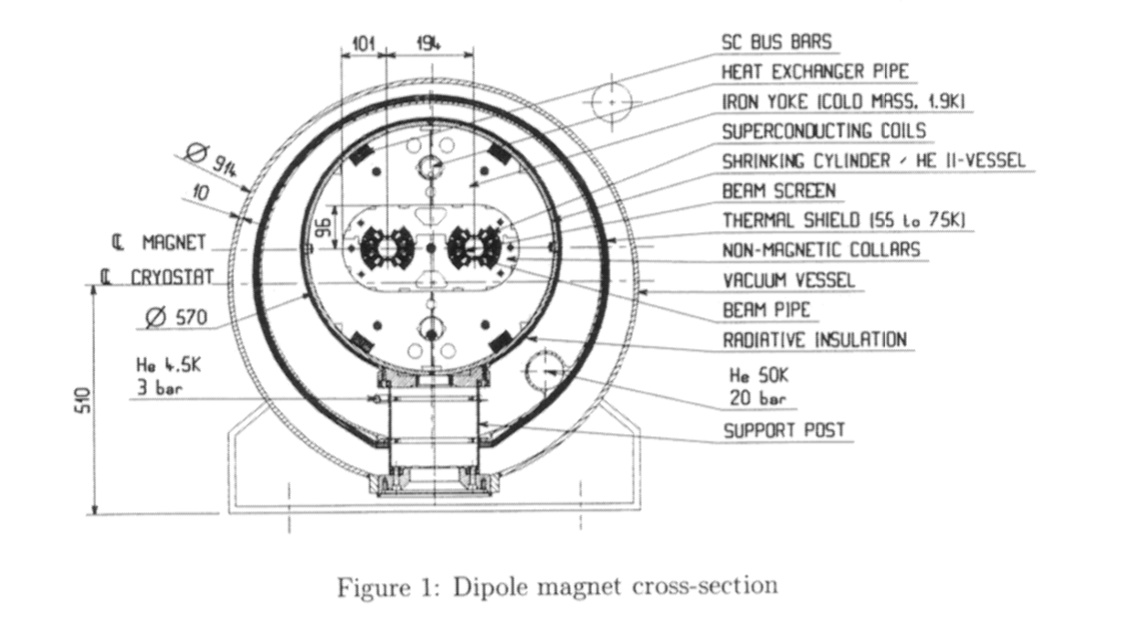
\includegraphics[width=0.75\textwidth]{figures/chapter_ATLAS/DipoleMagnets}
        \caption{
        The cross-section of the dipole magnet~\cite{Bruning:782076}.
        }
        \label{fig:dipole}
    \end{center}
\end{figure}

\subsubsection*{The Quadrupole Magnet}
The Quadrupole magnets are used in the LHC to focuses and defocuses the proton beams for collision. They are built in a way that is much like the main dipole, where single quadrupole magnet is capable of bending two proton beams. Figure~\ref{fig:quadrupole} shows a cross-section of the quadrupole magnet. 

\begin{figure}[!htb]
    \begin{center}
        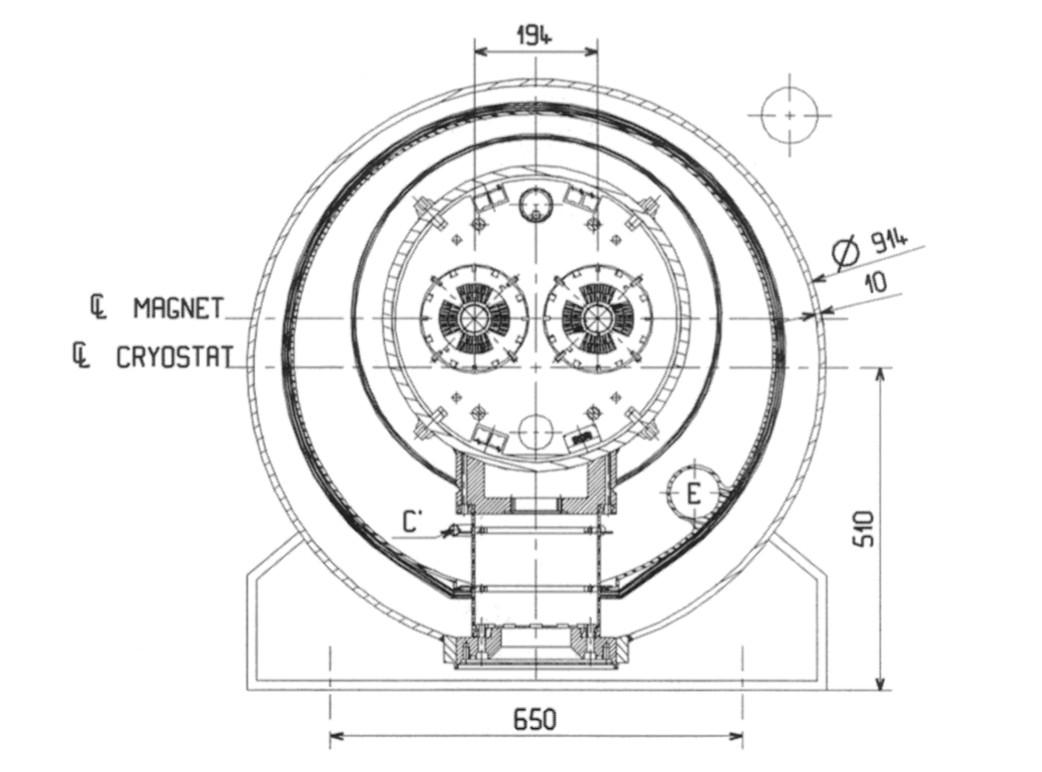
\includegraphics[width=0.75\textwidth]{figures/chapter_ATLAS/QuadrupoleMagnets}
        \caption{
            The cross-section of the quadrupole magnet~\ref{Bruning:782076}.
        }
        \label{fig:quadrupole}
    \end{center}
\end{figure}

\subsubsection*{The Sextupole and Dipole Corrector Magnet}
In addition, there are corrector magnets that correct for the field error of the main magnets mentioned above. More design details can be found in the conceptual design report of the LHC~\ref{Bruning:782076}.

\section{The ATLAS Detector}
\label{ATLAS}
The ATLAS detector is a general-purpose detector. It is the summation of a series of detector systems each produces different tracks to a particle. The ATLAS detector has a special emphasis on the muon system, as the dimuon final state was a main channel for the Higgs discovery. In the following sections, different parts of the detector will be discussed in detail. 

\begin{figure}[!htb]
    \begin{center}
        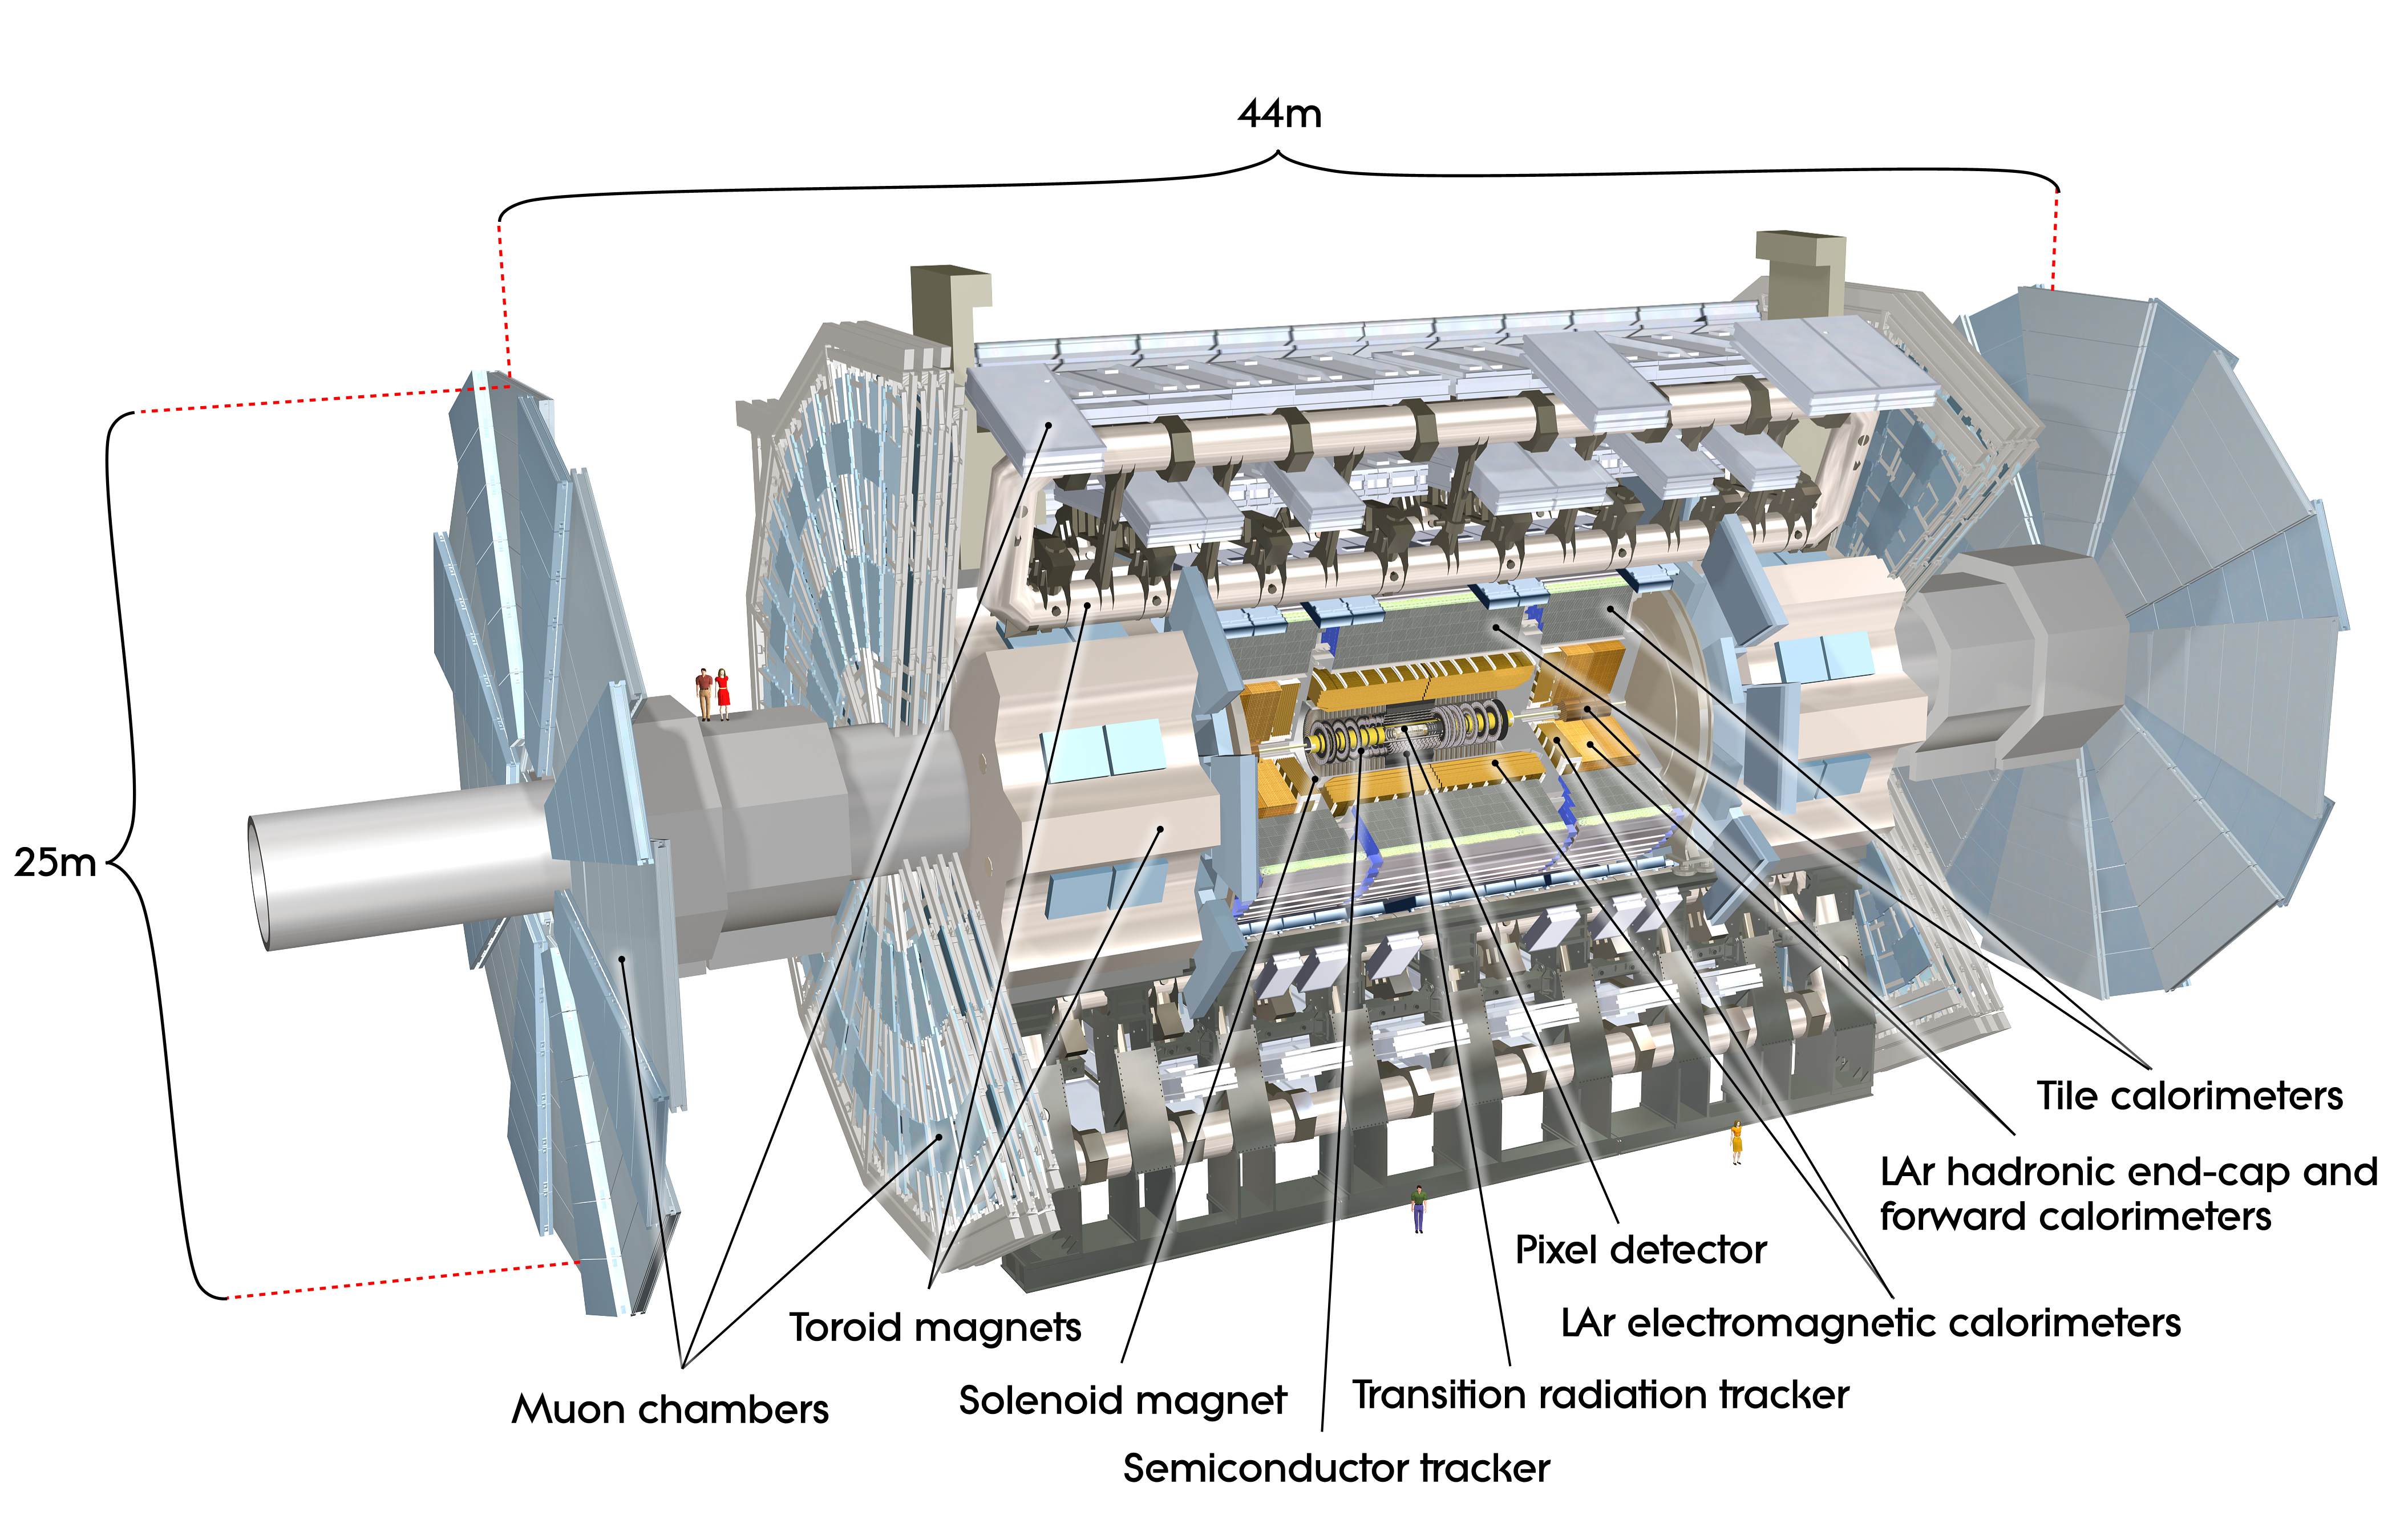
\includegraphics[width=0.75\textwidth]{figures/chapter_ATLAS/ATLASDetector}
        \caption{
			Computer generated image of the ATLAS detector\cite{Pequenao:1095924}. Showing the different parts of the components involved. 
        }
        \label{fig:ATLASDectector}
    \end{center}
\end{figure}


\subsection*{The ATLAS coordinate system}

The ATLAS detector uses a cylindrical coordinate system: Z-$\phi$-$\eta$ to describe the particles location after interactions.
The z-axis runs along the beamline and starts at the origin (center and middle) of the detector. The x-y plane perpendicular to the z-axis described as the transverse plane is represented in the polar coordinate~\ref{fig:Coordinates}. The plane is described by two angles: $\phi$ is the 2$\pi$ azimuthal angle on the x-y plane and the 1$\pi$ polar $\theta$ angle with respect to the z axis is given in term of psuedorapidity, the term is Lorentz invariant and is its conversion to theta is given
by Eq.~\ref{eq:Eta}. The $\delta R$ quantity is used to describe the angular distance between particles, it's defined in Eq.~\ref{eq:deltaR} This quantity is approximately Lorentz invariant. Figure~\ref{fig:Coordinates} shows the ATLAS coordinate system. Figure~\ref{fig:pseudorapidity} shows the pseudorapidity($\eta$) to angle conversion. 

\begin{equation}
    \eta=ln(tan(\theta/2))
    \label{eq:Eta}
\end{equation}

\begin{equation}
\delta R=\sqrt{\delta\eta^{2}+\delta\phi^{2}} 
\label{eq:deltaR}
\end{equation}

\begin{figure}[!htb]
    \begin{center}
        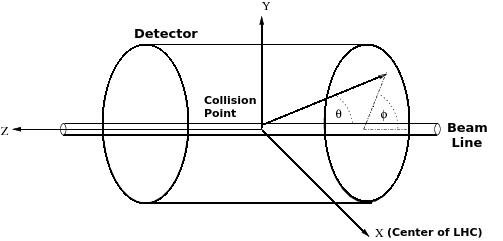
\includegraphics[width=0.75\textwidth]{figures/chapter_ATLAS/Coordinates}
        \caption{
            This figure displays the coordinate of the ATLAS detector system~\cite{2008}.
        }
        \label{fig:Coordinates}
    \end{center}
\end{figure}

\begin{figure}[!htb]
    \begin{center}
        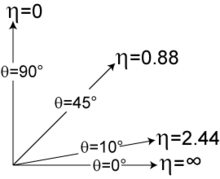
\includegraphics[width=0.75\textwidth]{figures/chapter_ATLAS/pseudorapidity}
        \caption{
            Pseudo-rapidity $\eta$ to angle in degree conversion~\cite{enwiki:1052183914}.
        }
        \label{fig:pseudorapidity}
    \end{center}
\end{figure}



\subsection{Inner Detector}
The inner detector(ID) is the innermost part of the ATLAS detector. Its main function is to record charged particle trajectories. The tracks provide valuable information for the reconstruction of the primary vertices of particle interactions. All four parts of the ID are enclosed by a superconducting solenoid magnet of 2T aligned along the beamline, charged particles are curved into helical trajectories along the beamline. This is be used for charge, mass and momentum calculation as well as particle
identification. 

% TODO insert charge to mass trajectory calculation


The inner detector is made up of four different parts. From inside out, the Insertable B Layer, the Pixel detector, the Semi-Conductor Tracker(SCT) and the Transition Radiation Tracker(TRT). 
Its resolution is the highest in the innermost part of the detector and decreases outward. The following is a detailed description of the four parts of their coverage and detector mechanism. 

Closest to the core of the detector is a very high-resolution insertable B layer(IBL). It was inserted after Run I to further extend the pixel detector coverage to $|\eta|< 2.9$. This helps with b-hadron identification through better vertex reconstruction.

Around the IBL is the Pixel detector. It is made of three layers of fine silicon pixels of spatial resolution of 10$\mu$ m in the r-$\phi$ direction and 115$\mu$ m in the z-direction. It provides a cylindrical coverage that covers up to $|eta|<2.5$. Electron-hole pairs are generated when charged particle passes through the silicon pixel which the signal is then read out through the applied electric field.
Surrounding the pixel detector, there is a silicon microstrip detector called the Semi-Conductor Tracker (SCT), located in radii between 30-51 cm, which is made up of 4 layers of strip silicon sensor. Each SCT layer is made up of two overlapping sets of silicon strips at an angle with one another. The working mechanism of the detector is similar to that of the pixel detector, but the resolution is slightly reduced to 17 $\mu$m in the r-$\phi$ plane and 580 $\mu$ m along the z-axis. 
The outermost part of the ID is called the Transition Radiation Tracker(TRT), made up of gas-filled straws. There are 70 layers in the barrel and 140 layers in each end cap covering up to $|\eta|<2.0$. Each straw tube contains gas that can be ionized by charged particles, the electron formed in the process will then move toward the charged center of the straw to be read out for momentum, trajectory and charge calculation. The TRT also helps with particle identification, as charged particles alsoemit a photon and this probability is related to the Lorentz factor. Lower mass electrons emit more photons than charged hadrons. Therefore, this can be used to identify electrons over hadrons on top of track reconstruction. The TRT has a resolution of 130$\mu$ m in the r-$\phi$ plane.

\begin{figure}[!htb]
    \begin{center}
        \includegraphics[width=0.4\textwidth]{figures/chapter_ATLAS/InnerDetector1}
        \caption{
            This image shows the computer generated image of the inner detector~\cite{Pequenao:1095926}.
        }
        \label{fig:InnerDetector}
    \end{center}
\end{figure}

\begin{figure}[!htb]
    \begin{center}
        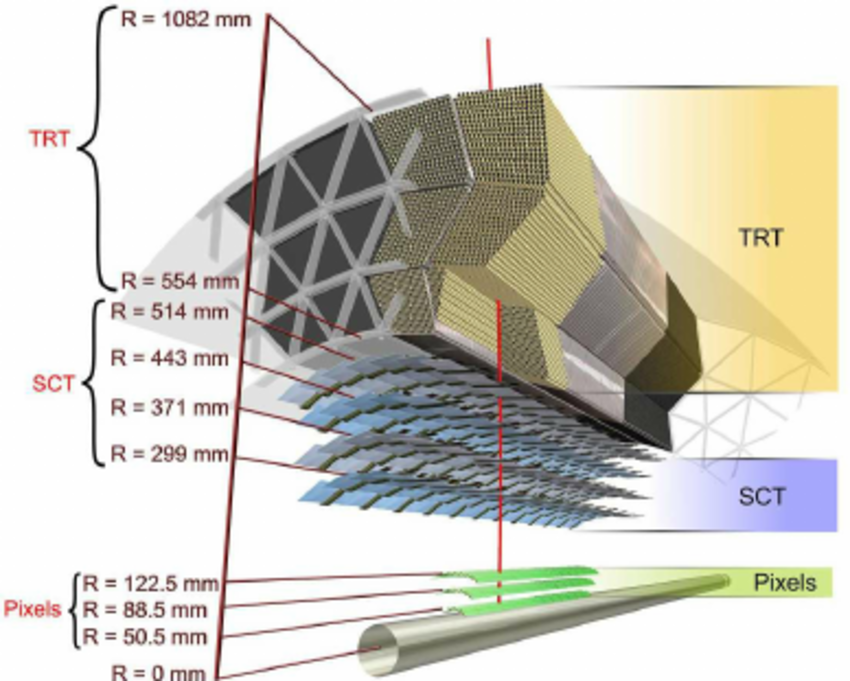
\includegraphics[width=0.75\textwidth]{figures/chapter_ATLAS/InnerDetector2}
        \caption{
            This image shows the computer generated image of the inner detector and its inner layout~\cite{Pequenao:1095926}.
        }
        \label{fig:InnerDetector2}
    \end{center}
\end{figure}

\subsection{Calorimeter}
The main function of the calorimeter is to provide energy measurement for particles. The ATLAS Calorimeter is split into two parts, sorted by the particle interaction method, The Electromagnetic-Calorimeter(E-Cal) utilizes the electromagnetic interaction and measures energy deposit in the form of electron and photon showers; the Hadronic Calorimeter uses strong hadronic interactions, energy is measured in the form of a hadronic shower in quarks and gluons. Both systems utilize a dense passive material for the particle showering and are sampled through a layer of sensitive active element for detection. Below, different components of the ECAL and the HCAL will be described in detail. 

After tracking, the particle will first reach the ECAL. The first layer is the liquid-argon(LAr) electromagnetic(EM) calorimeter. The passive medium for showering is lead. The endcap portion covers $1.375< |\eta| < 3.2$, and the barrel cover up to $|\eta|<1.475$. The innermost layer has the greatest granularity of 0.003, the second layer has a resolution of 0.025 and the third layer is the most coarse. 

The hadronic calorimeter(HCAL) measures hadron showering in the form of quarks and gluons, the barrel portion is made of a tile calorimeter, it uses steel as the passive element for showering and scintillating tiles as the readout active element and the 

The forward calorimeter end cap uses LAr for both the ECAL and HCAL, but copper-tungsten is used as the passive layer instead. 


\begin{figure}[!htb]
    \begin{center}
        \includegraphics[width=0.75\textwidth]{figures/chapter_ATLAS/Calorimeter}
        \caption{
            This image shows the computer generated image of the calorimeter and its inner layout~\cite{Pequenao:1095927}.
        }
        \label{fig:Calorimeter}
    \end{center}
\end{figure}

\subsection{Muon Spectrometers}
The muon spectrometer(MS) measures both the trajectory of muons and perform their triggering. The only type of particles that make it past the calorimeters and reach the muon spectrometer are either non-interacting particles, or they are the minimum ionizing particles, muons. Tracking and measurement of muons can effectively distinguish them from the non-interacting particle which could be neutrinos or beyond the standard model physics particles like dark matter. 
The muon spectrometer system of ATLAS is surrounded by the superconducting toroid magnets, the barrel toroid provide up to 0.5 T between $1.6 < |\eta|<2.7$ , the end cap toroids provide up to 1T. The magnet bends the particles along the beamline into the end caps.
For precision tracking, the muon system is made up of the Monitored Drift Tubes(MDTs) in both the barrel and the endcap region, in the forward region there is a Cathode Strip Chamber(CSCs) in region $|\eta|>2.7$
For triggering, it uses the Resistive Plate Chamber(RPC) in the barrel and the Thin Gap Chambers (TGCs) in the end cap for fast readout. 

%Comparison with CMS

\begin{figure}[!htb]
    \begin{center}
        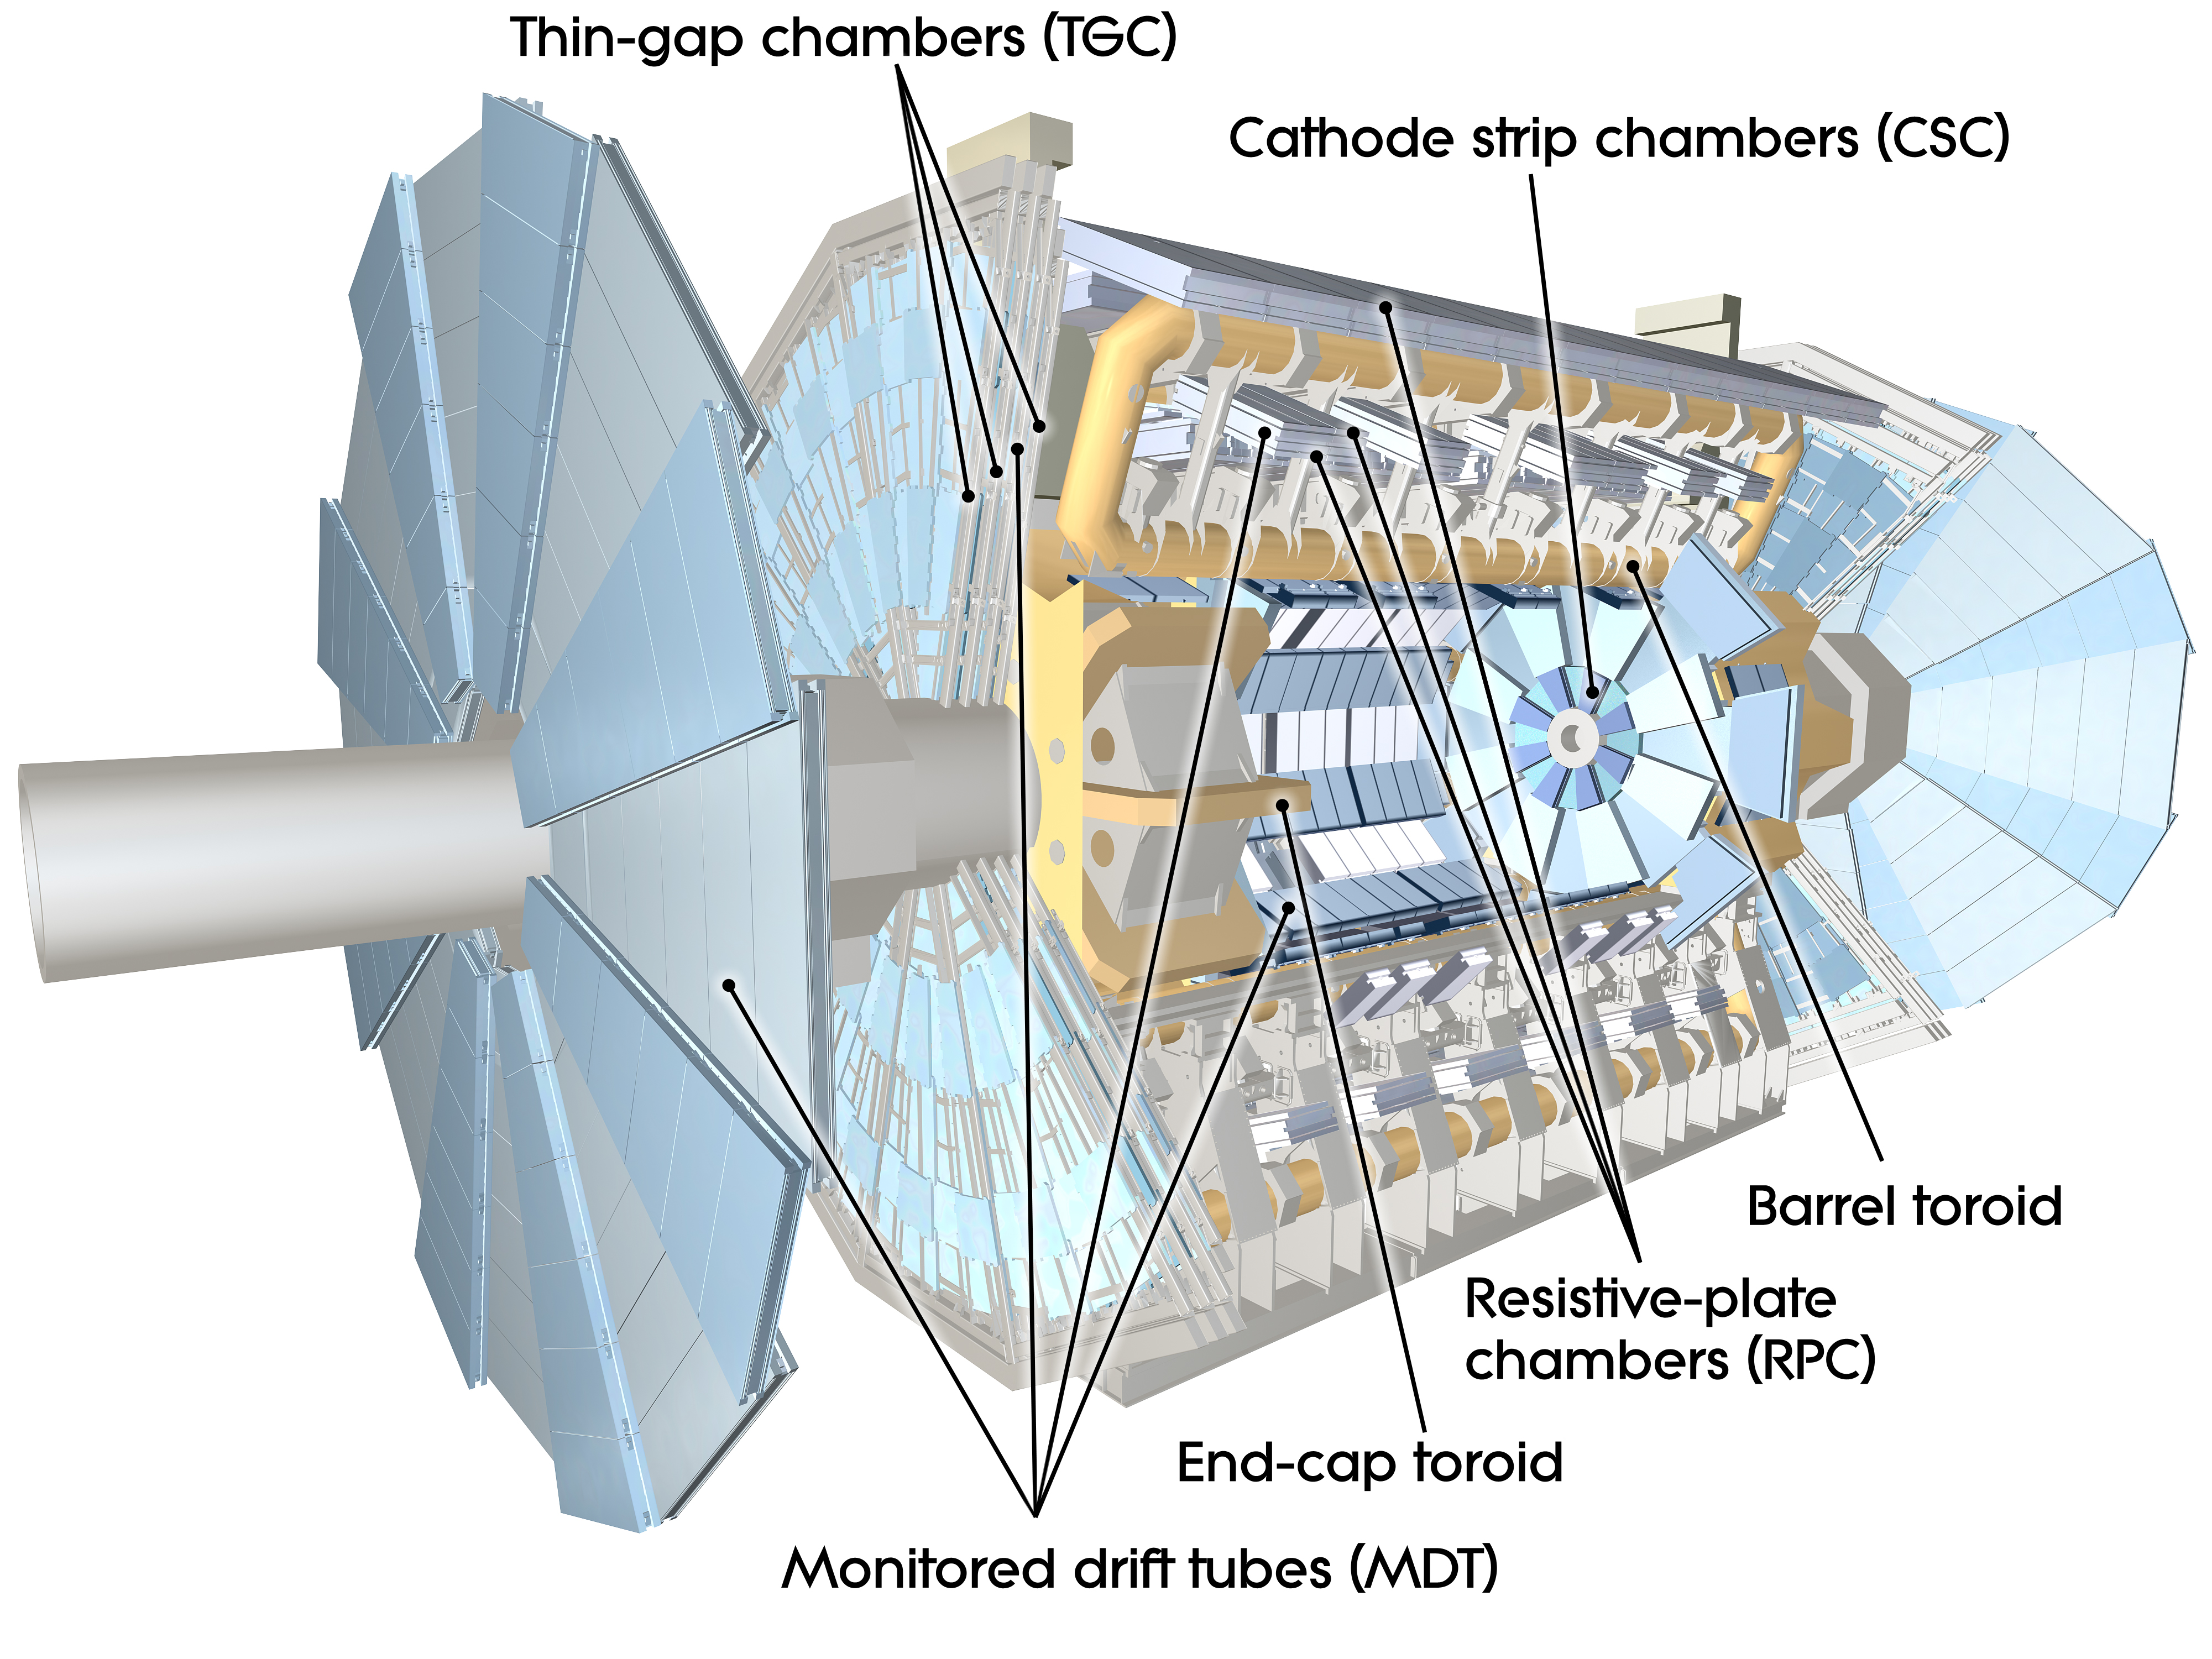
\includegraphics[width=0.75\textwidth]{figures/chapter_ATLAS/MuonSpectrometer}
        \caption{
            This image shows a computer generated image of the muon spectrometer~\cite{Pequenao:1095929}.
        }
        \label{fig:MuonSpectrometer}
    \end{center}
\end{figure}

\section{Data Acquisition of ATLAS}
\label{trigger}
%Data acquisition of ATLAS 
During Run II, the LHC performed proton-proton collision at $\sqrt{s}=13 TeV$ at the instantaneous luminosity of $10^{34}cm^{-2}s^{-1}$. An approximate of 33.7 pp interaction per bunch crossing was delivered. 
At this collision rate, not all data could be processed and saved. The process of selecting experimentally interesting events is called ``triggering". In Run II, triggering is administered and controlled by a central trigger processor which assigns different information from detectors to different part of the trigger computing system. There are two levels of triggering in ATLAS Run II, the low level hardware-based trigger is called L1 triggers, the second level software based high level triggering is called the High-level trigger(HLT). 
The L1 trigger filters through the input at 40 MHz to 100kHz. This is done by looking at energy deposits at the calorimeters that could be
candidate leptons, jets, or photons. Muons are triggered by the hits that formed towers in the MS system. 
Events that pass through the L1 trigger will then be passed onto the HLT. The HLT further filters the 100kHz events received to 1kHz for writing to disk for offline analysis. The HLT is software-based it further defines region-of-interest in detector and filter events that do not fit the trigger selection criteria. High-level objects are created from
the online information and an event loop is used to discard events that do not fulfill the trigger criteria.
Events are saved to ``trigger chains" for later analyses, they are sorted into different analysis derivations with basic criteria applied for different types of analyses. 

\begin{figure}[!htb]
    \begin{center}
        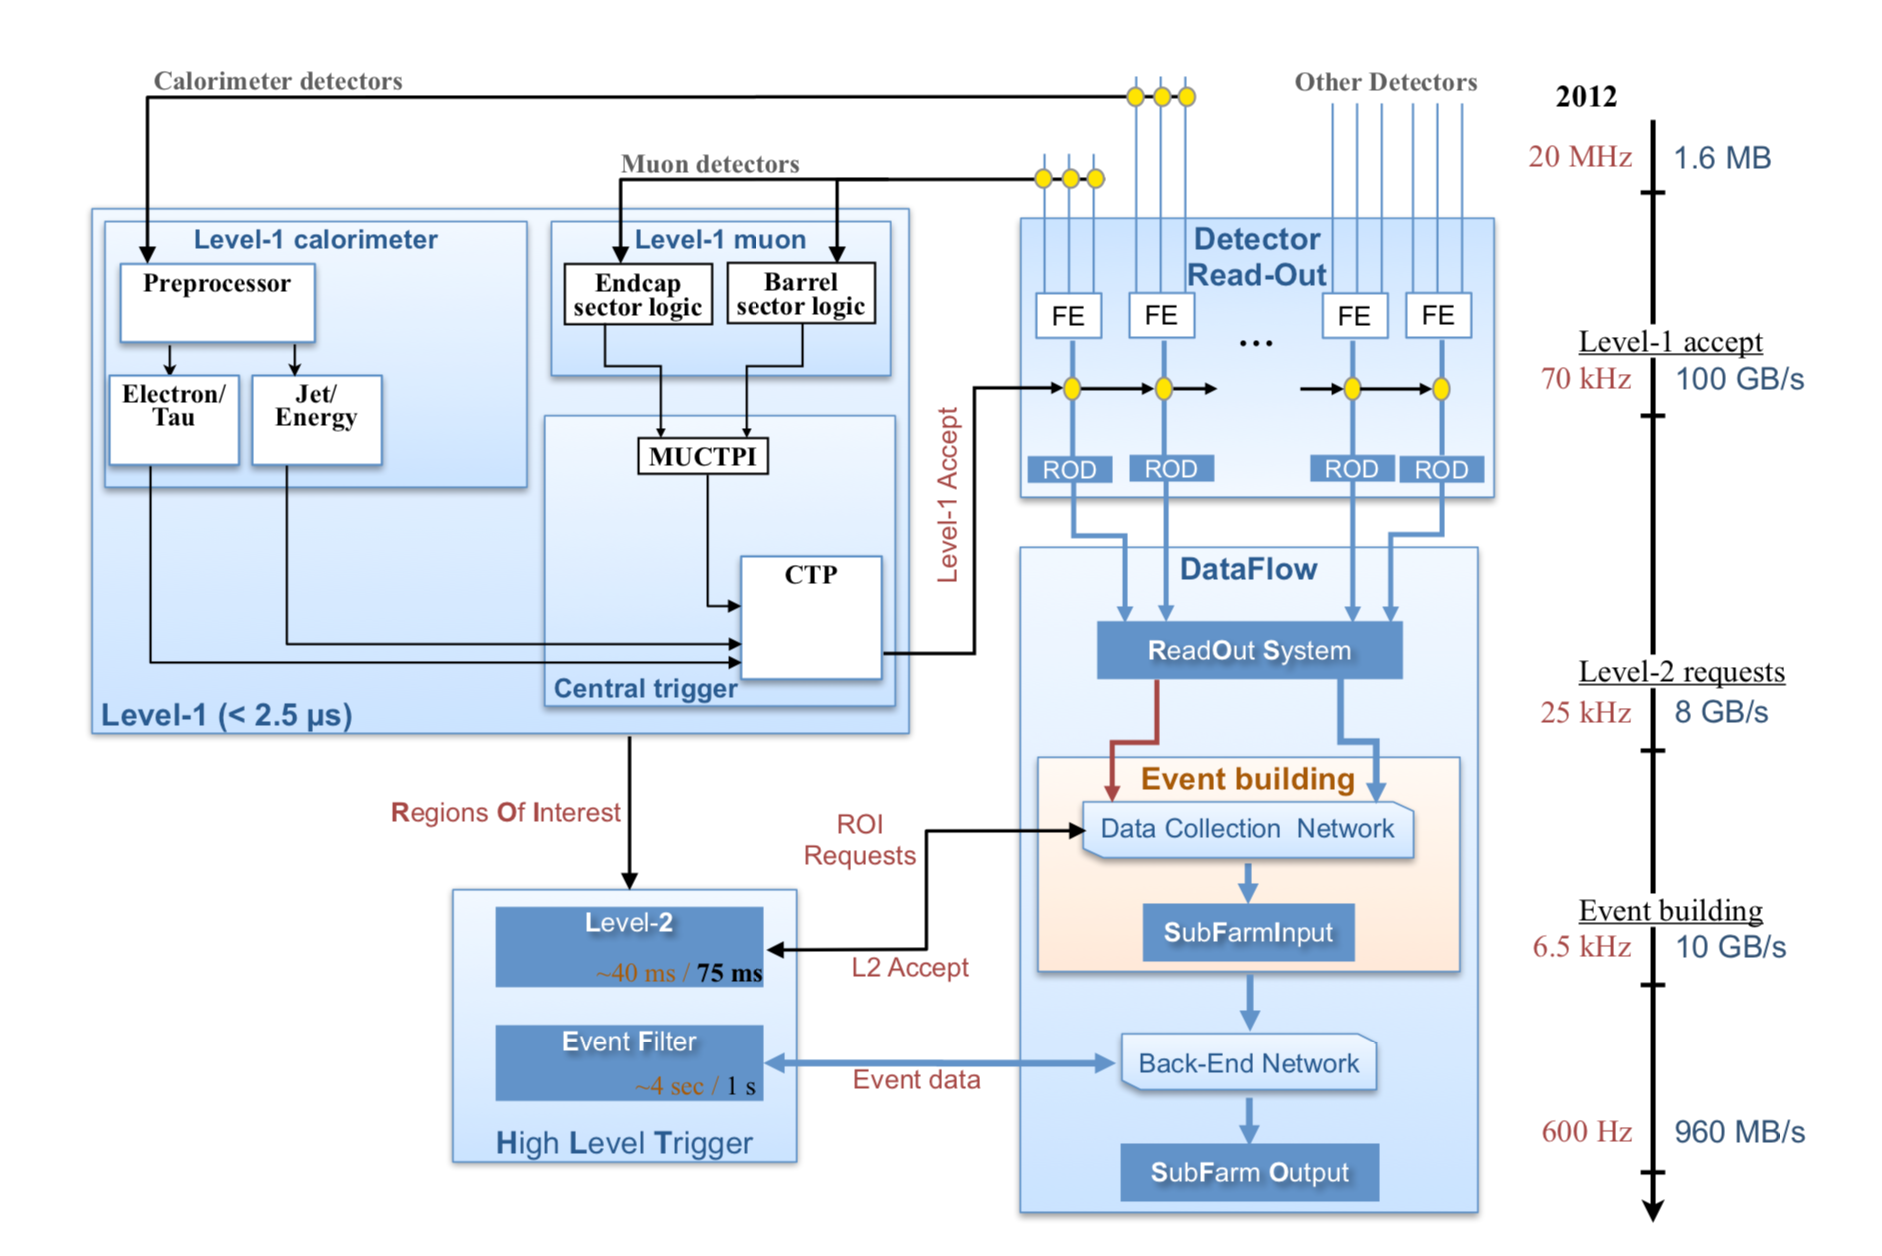
\includegraphics[width=0.75\textwidth]{figures/chapter_ATLAS/TDAQ}
        \caption{
            This image shows the schematic overview of the ATLAS triggering system~\cite{Pequenao:1095929}.
        }
        \label{fig:TDAQ}
    \end{center}
\end{figure}


\include{sections/chapter_CommonAnalysisItems}
\include{sections/chapter_Insitute_Jet_Calibration}
\chapter{the New Small Wheel Upgrade}
\label{chapter:NSW}


0. Introduction

1. Boosted resonance finding

2. Particle definition

3. Statisitcal method  



0. Introduction

1. Boosted resonance finding

2. Particle definition

3. Statisitcal method  

\chapter{The Resonance Search on the Dimuon Signature}
\label{chapter:dimuon}

\section{Introduction}

    % Why this is interesting  
    Owing to its unprecedented high energy, the run I and early run II of ATLAS has long focused on the high mass resonances searches. This has left some gaps in the low mass region that are unexplored. In the two lepton final state, there has been an analysis after the Z boson peak since the beginning of Run 1, however the mass region below the Z mass peak has left a region totally uncovered on ATLAS.

\begin{figure}[!htb]
    \begin{center}
        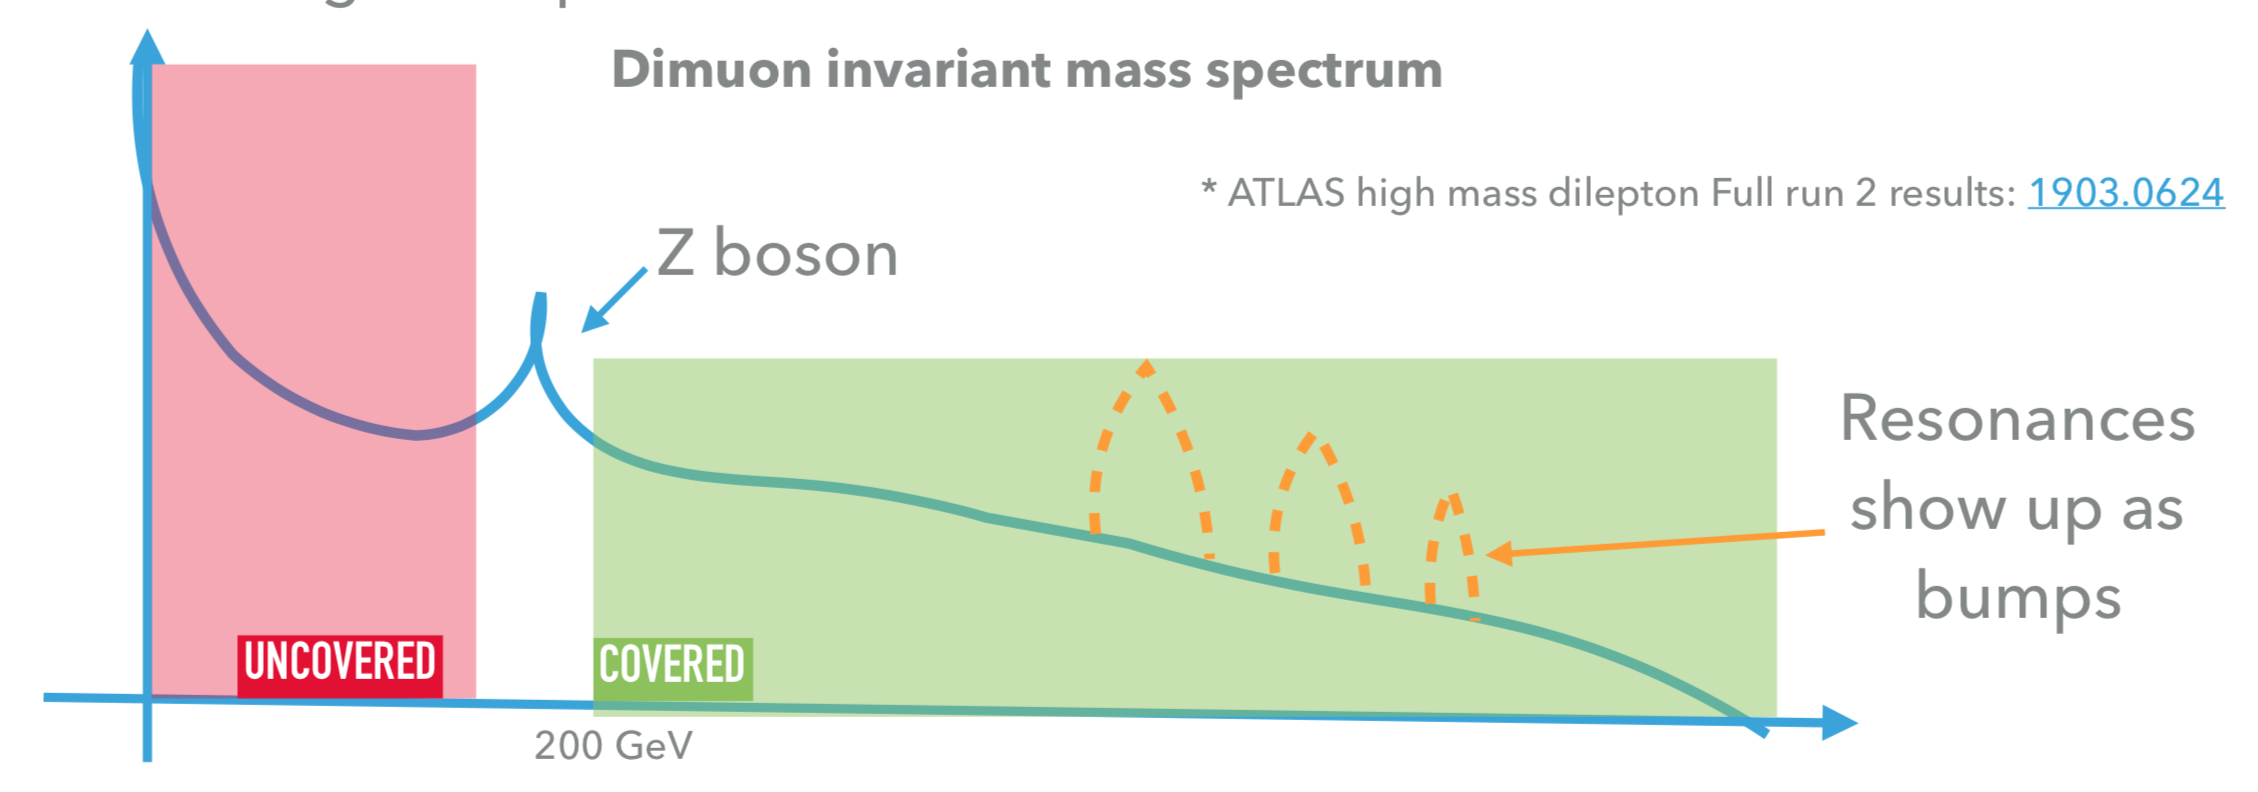
\includegraphics[width=0.75\textwidth]{figures/chapter_dimuon/dimuonStudies}        
        \caption{
        This cartoon illstrate the target signal region of the analysis and how it has not been covered by the previous high-mass dilepton analysis. }
            \label{fig:dimuonstudies}
    \end{center}
\end{figure}
   
    Since ATLAS collide partons, there are fewer background on leptons than jet processes, this allows lower transverse momentum lepton events to be saved. Using two muons as the resonance final state items, lower mass resonances can be searched for, going below the limits of the dijet resonances. The signal significance would be higher compared to jet. 

    This search results is interesting to the theoretical community for the dark matter benchmark interpretation possible.

%\section{Historical searches}    
%    Previous searches has been done directly in Tevatron experiment. Indirect constraints has been made in LEP as well. 
%
%    CMS results and tevatron results: 
%    
%    This study will be an independent finding from ATLAS and the first search done in this region.  


\section{The Search Channels}
Since there is a trigger turn-on feature near 45 GeV in the distribution due to the cut in muon transverse momentum in trigger, 
This analysis is based on a pheno-study first done here\cite{2014}.

There are two search channels in the analysis, each covering a different mass region, namely the boosted and the 

\begin{figure}[!htb]
    \begin{center}
        \includegraphics[width=0.75\textwidth]{figures/chapter_dimuon/turnedon}
        \caption{
        this figure shows the trigger turn on curve in the inclusive dimuon channel, and how utilizing the boosted channel a smooth background is possible in the lower mass region from 10-45 gev. samples used here are from the monte carlo sample in section~\ref{}, a minimal cut of muon pt >14 gev are done on the two leading muons. }
            \label{fig:turnon}
    \end{center}
\end{figure}

\section{Signal Theoretical Model}

    The analysis uses the dark matter LHC benchmark model and dark photon model outlined in~\ref{sec:LHCDM}.
Other models that are of interest and can be searched for in this analysis includes the W', the quantum blackholes,and axion models. 
The following search focuses on the search on the vector dilepton signature from the dark photon model and the dark matter benchmark. But as Gaussian limits are also set, the results will be reinterpretable for many other models that predicts scalar or axion-vector resonances. 

\begin{figure}[!htb]
    \begin{center}
        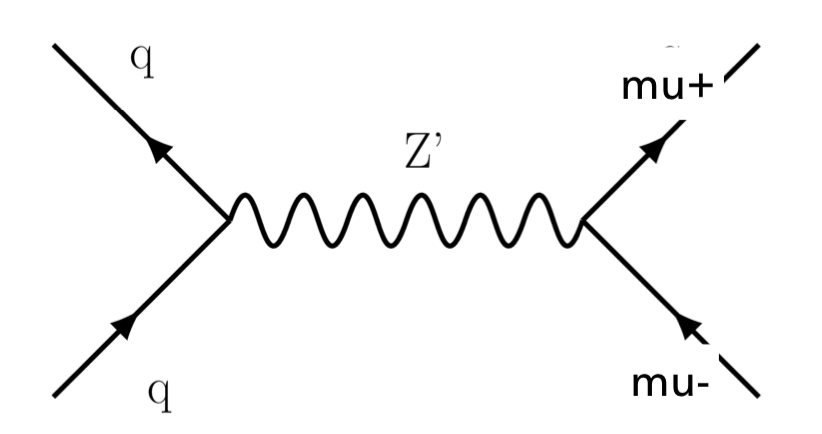
\includegraphics[width=0.75\textwidth]{figures/chapter_dimuon/dimuonFeynman}
        \caption{
            This figure shows the Feynmann diagram of the inclusive dimuon signal as the signal for the analysis. }
            \label{fig:dimuonFeynmann}
    \end{center}
\end{figure}


\begin{figure}[!htb]
    \begin{center}
        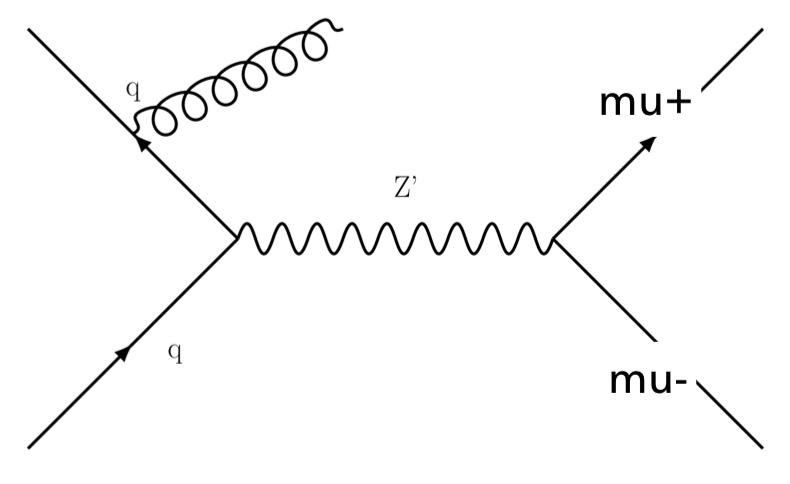
\includegraphics[width=0.75\textwidth]{figures/chapter_dimuon/dimuonISRFeynmann}
        \caption{
        This figure shows the Feynmann diagram of the boosted dimuon ISR signa used as the signal for the analysis. }
            \label{fig:dimuonFeynmann}
    \end{center}
\end{figure}

    The different signal distributions across different kinematics are shown here. 

\begin{figure}[!htb]
    \begin{center}
        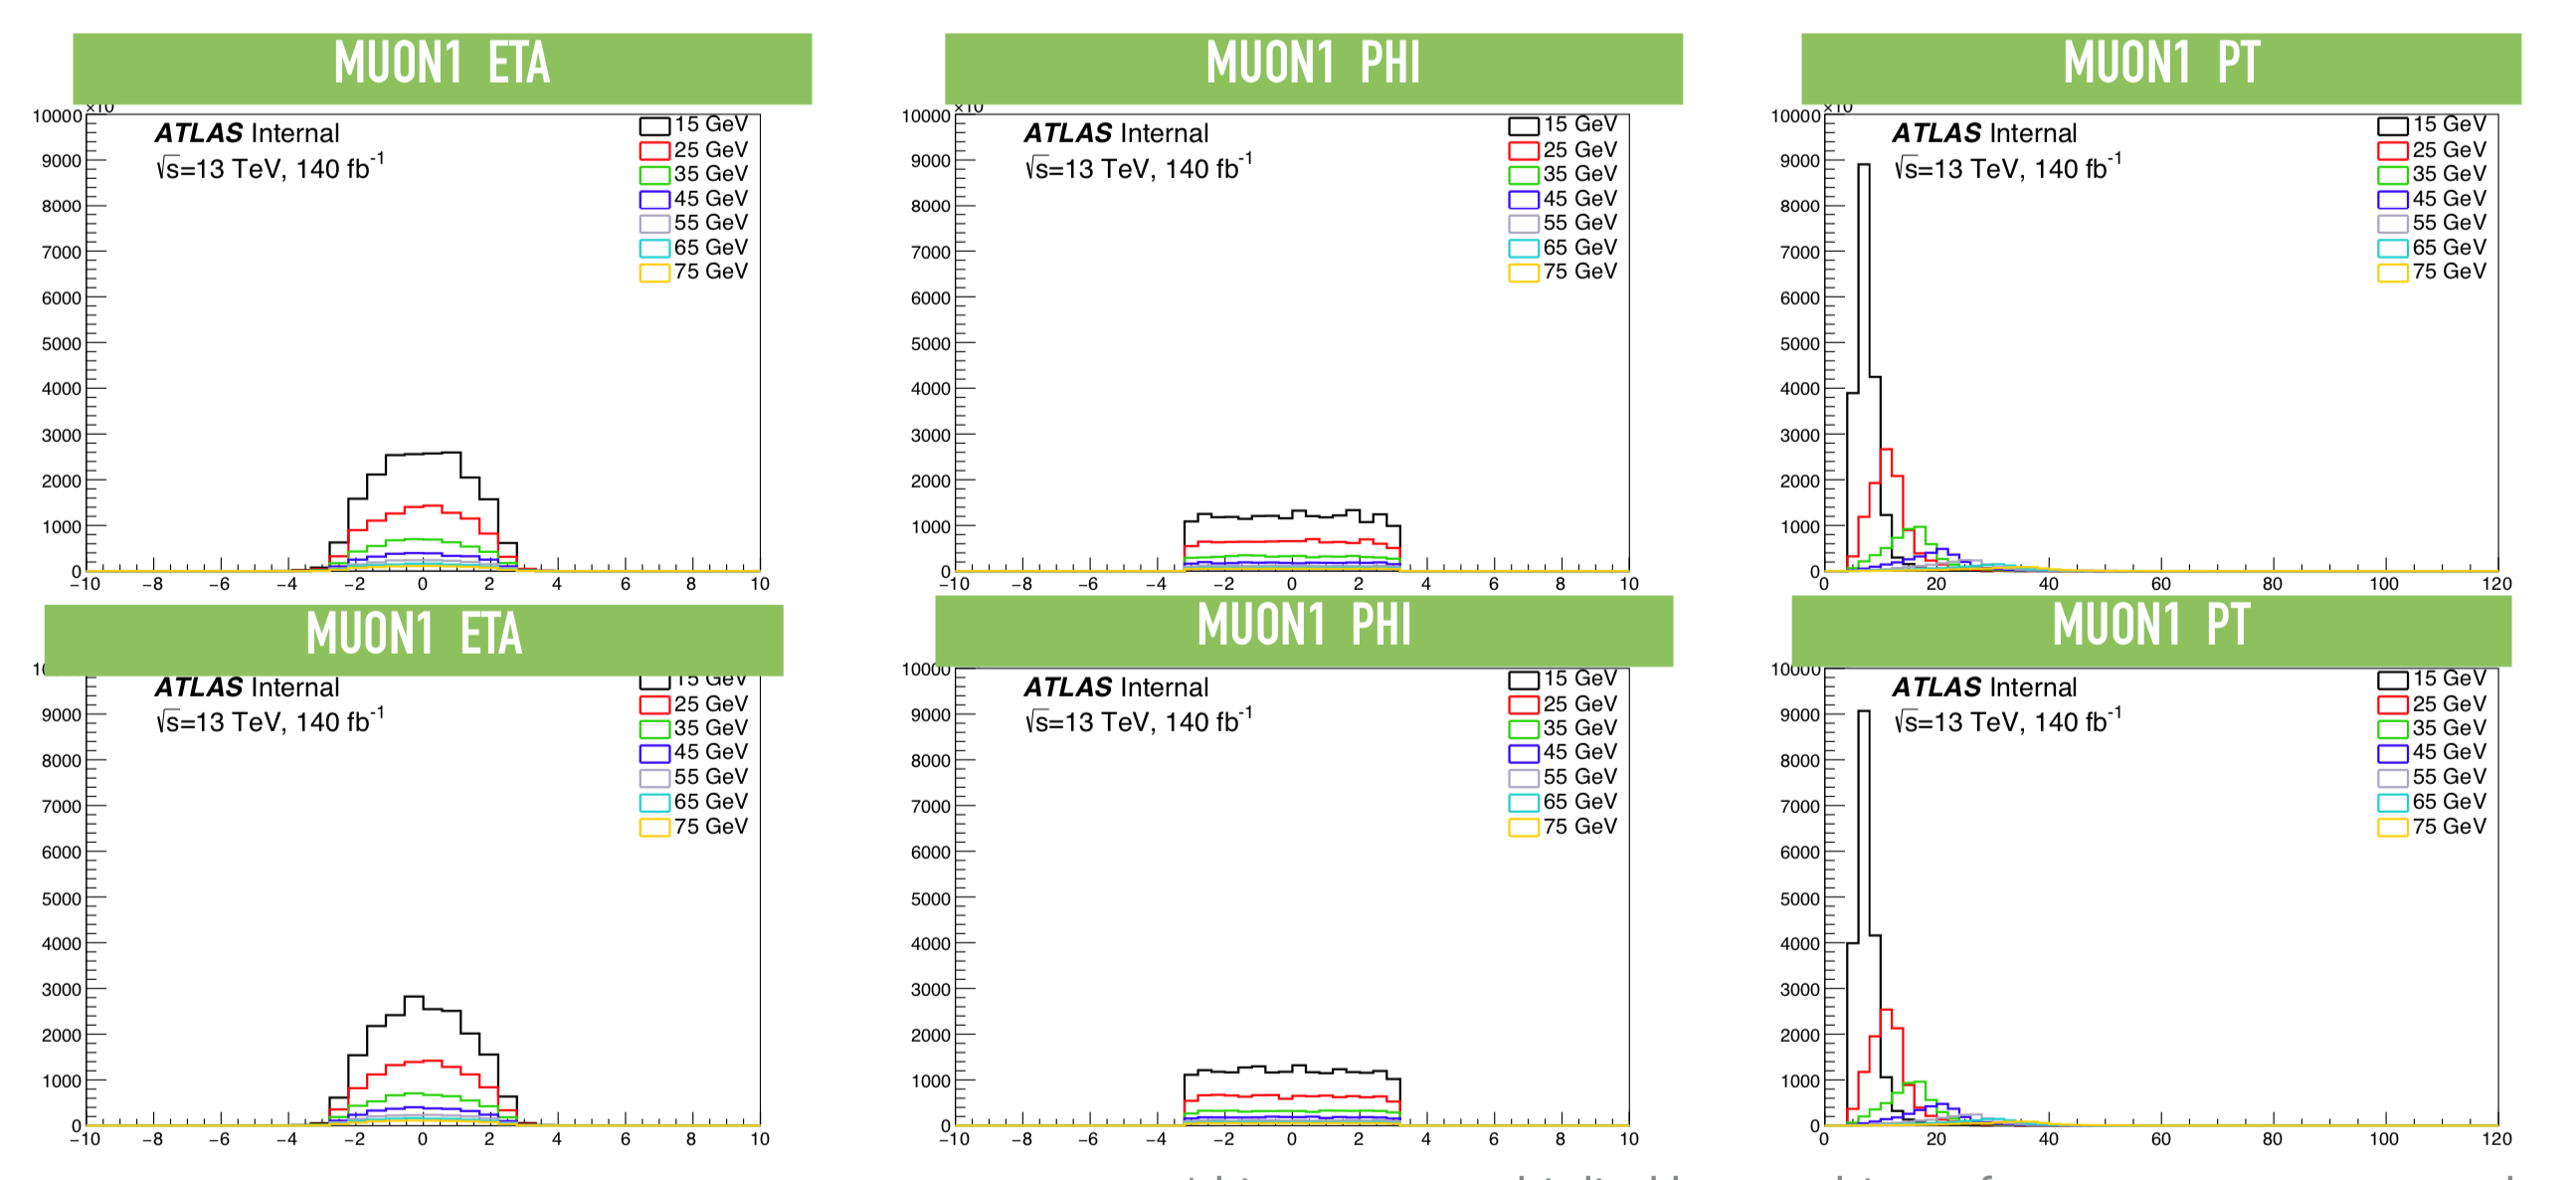
\includegraphics[width=0.75\textwidth]{figures/chapter_dimuon/dimuondist1}
        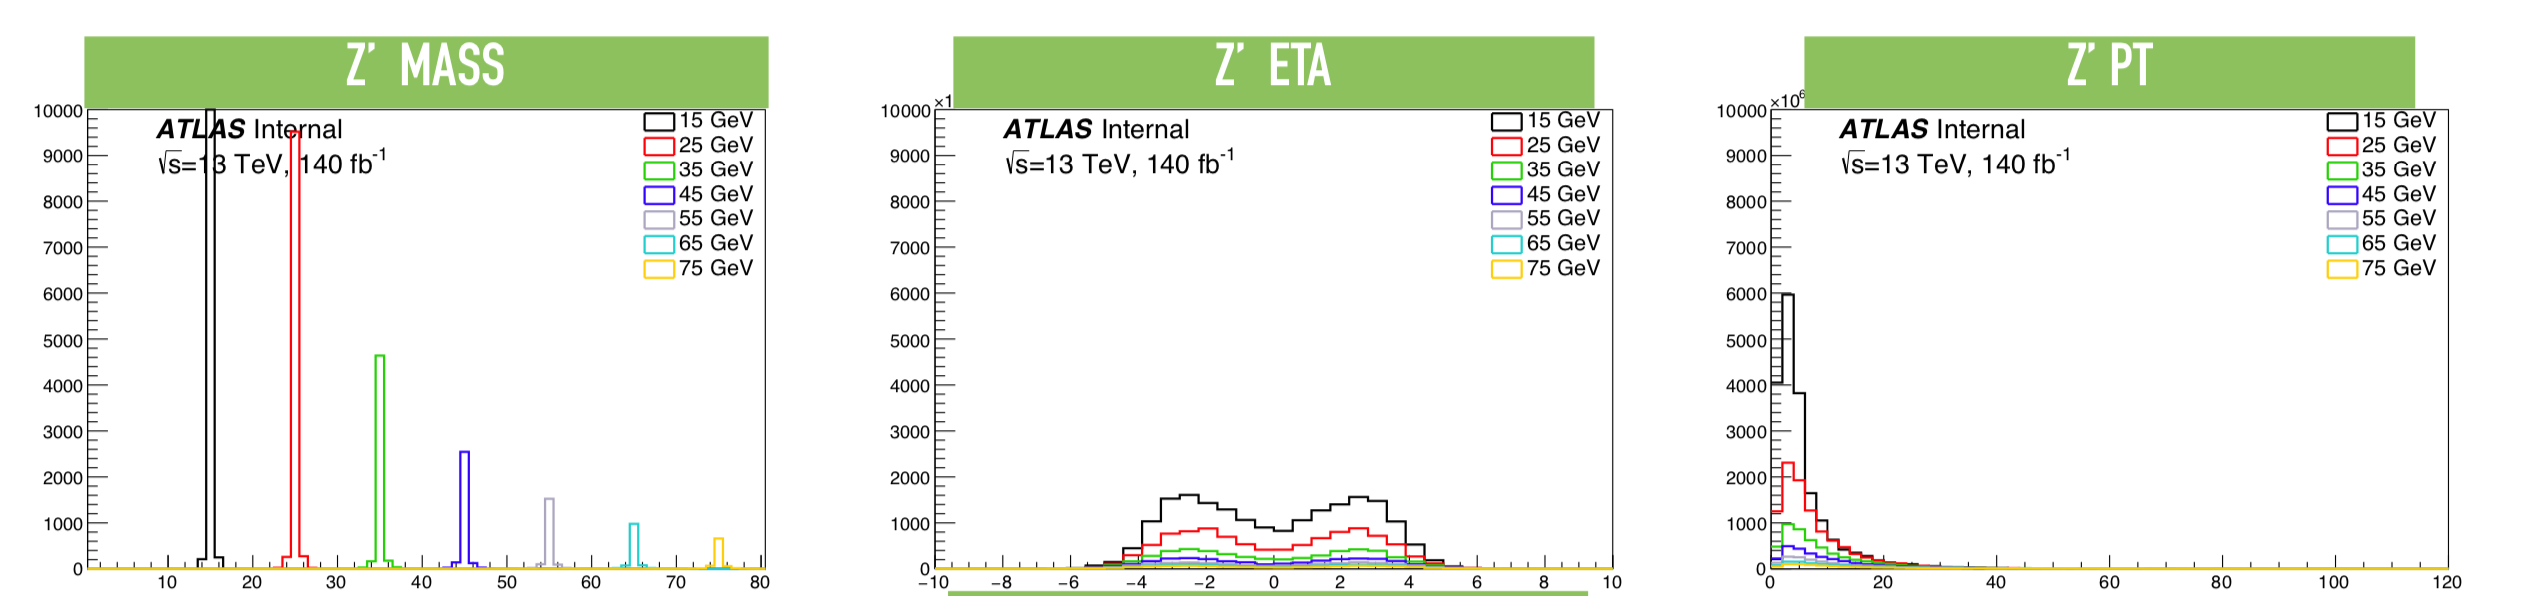
\includegraphics[width=0.75\textwidth]{figures/chapter_dimuon/dimuondist2}
        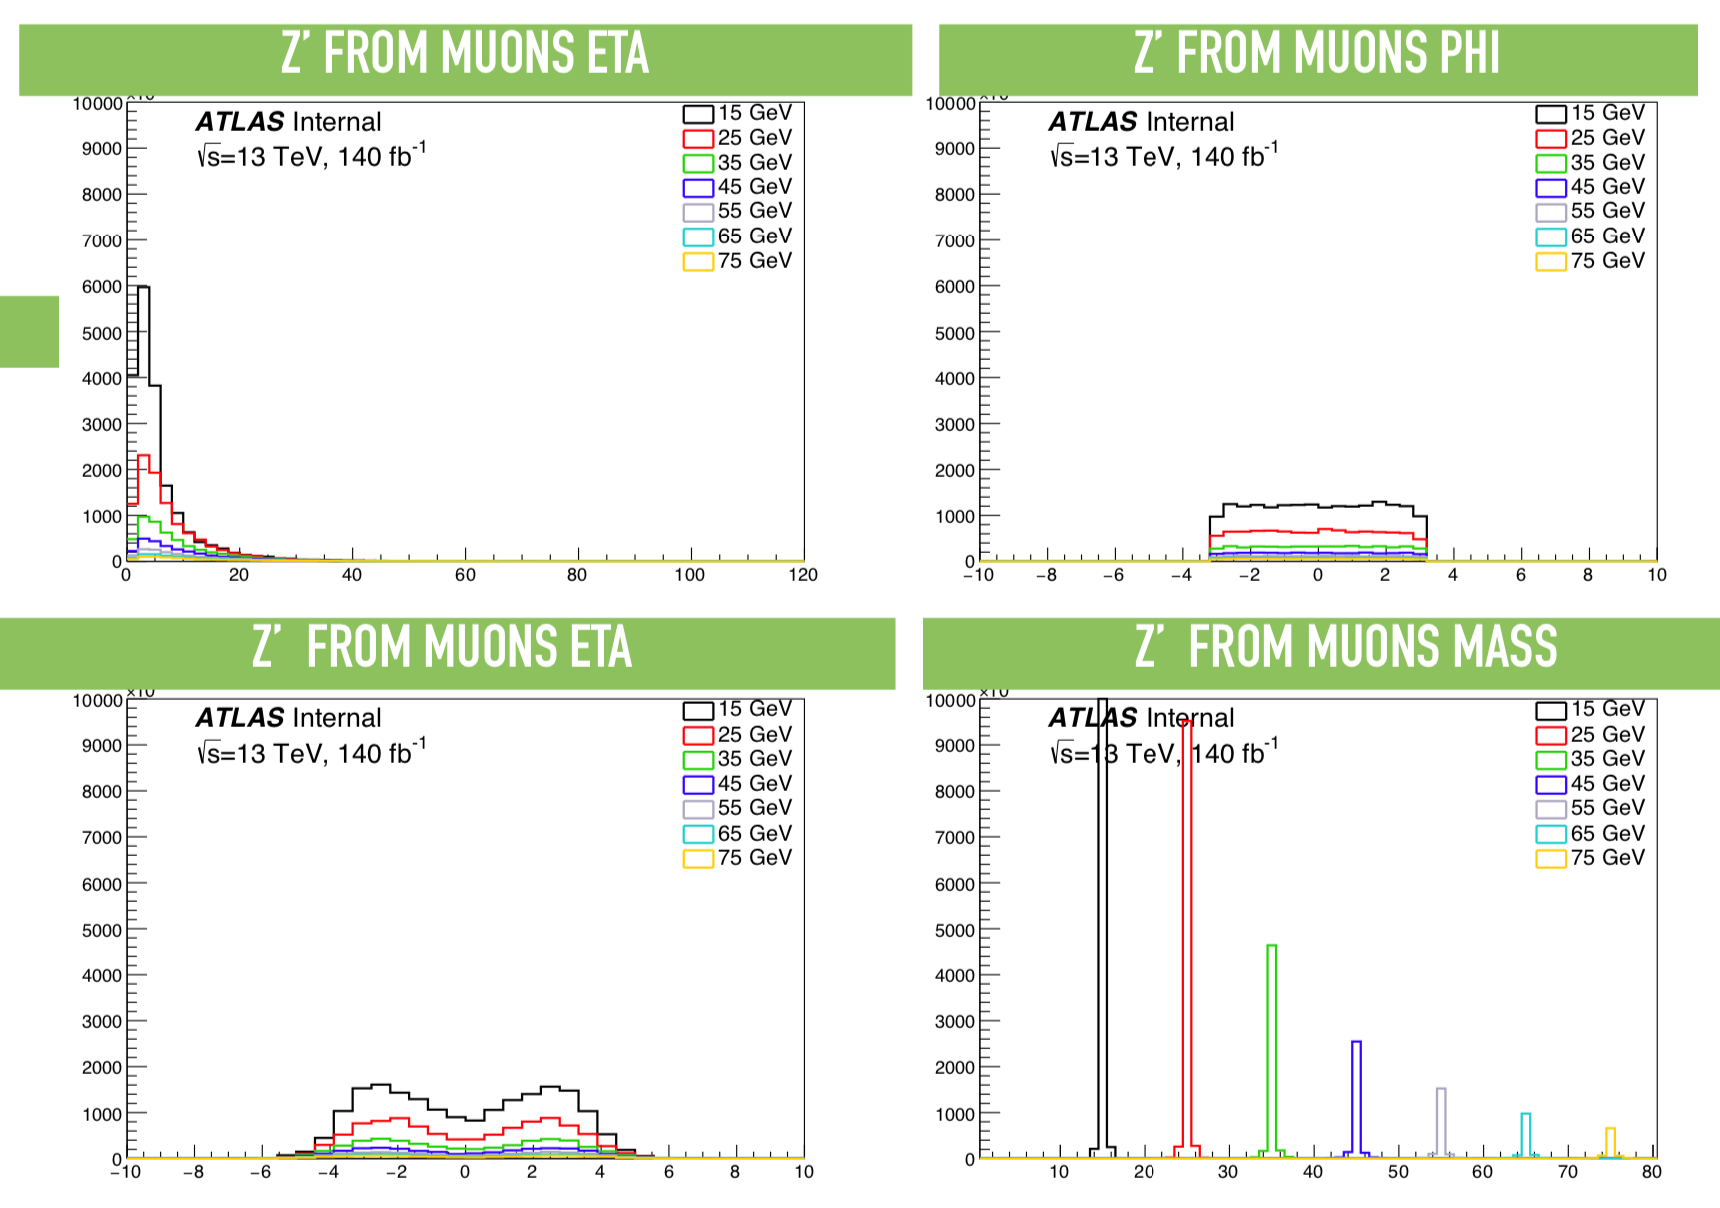
\includegraphics[width=0.5\textwidth]{figures/chapter_dimuon/dimuondist3}
        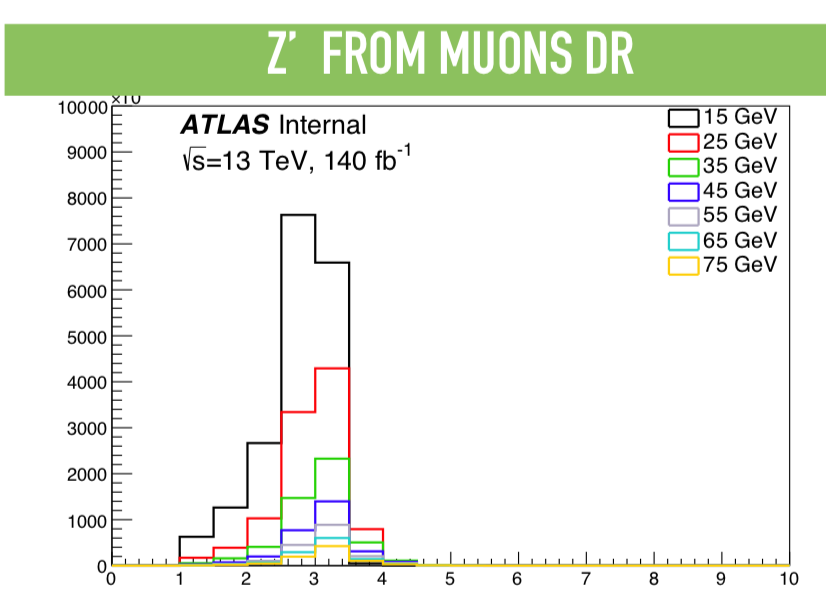
\includegraphics[width=0.2\textwidth]{figures/chapter_dimuon/dimuondist4}
        \caption{
        This figure shows the signal distribution of the inclusive dimuon samples generated. A minimal cut of muon pt >14 gev are done on the two leading muons. }
        \label{fig:dimuon}
    \end{center}
\end{figure}


\begin{figure}[!htb]
    \begin{center}
        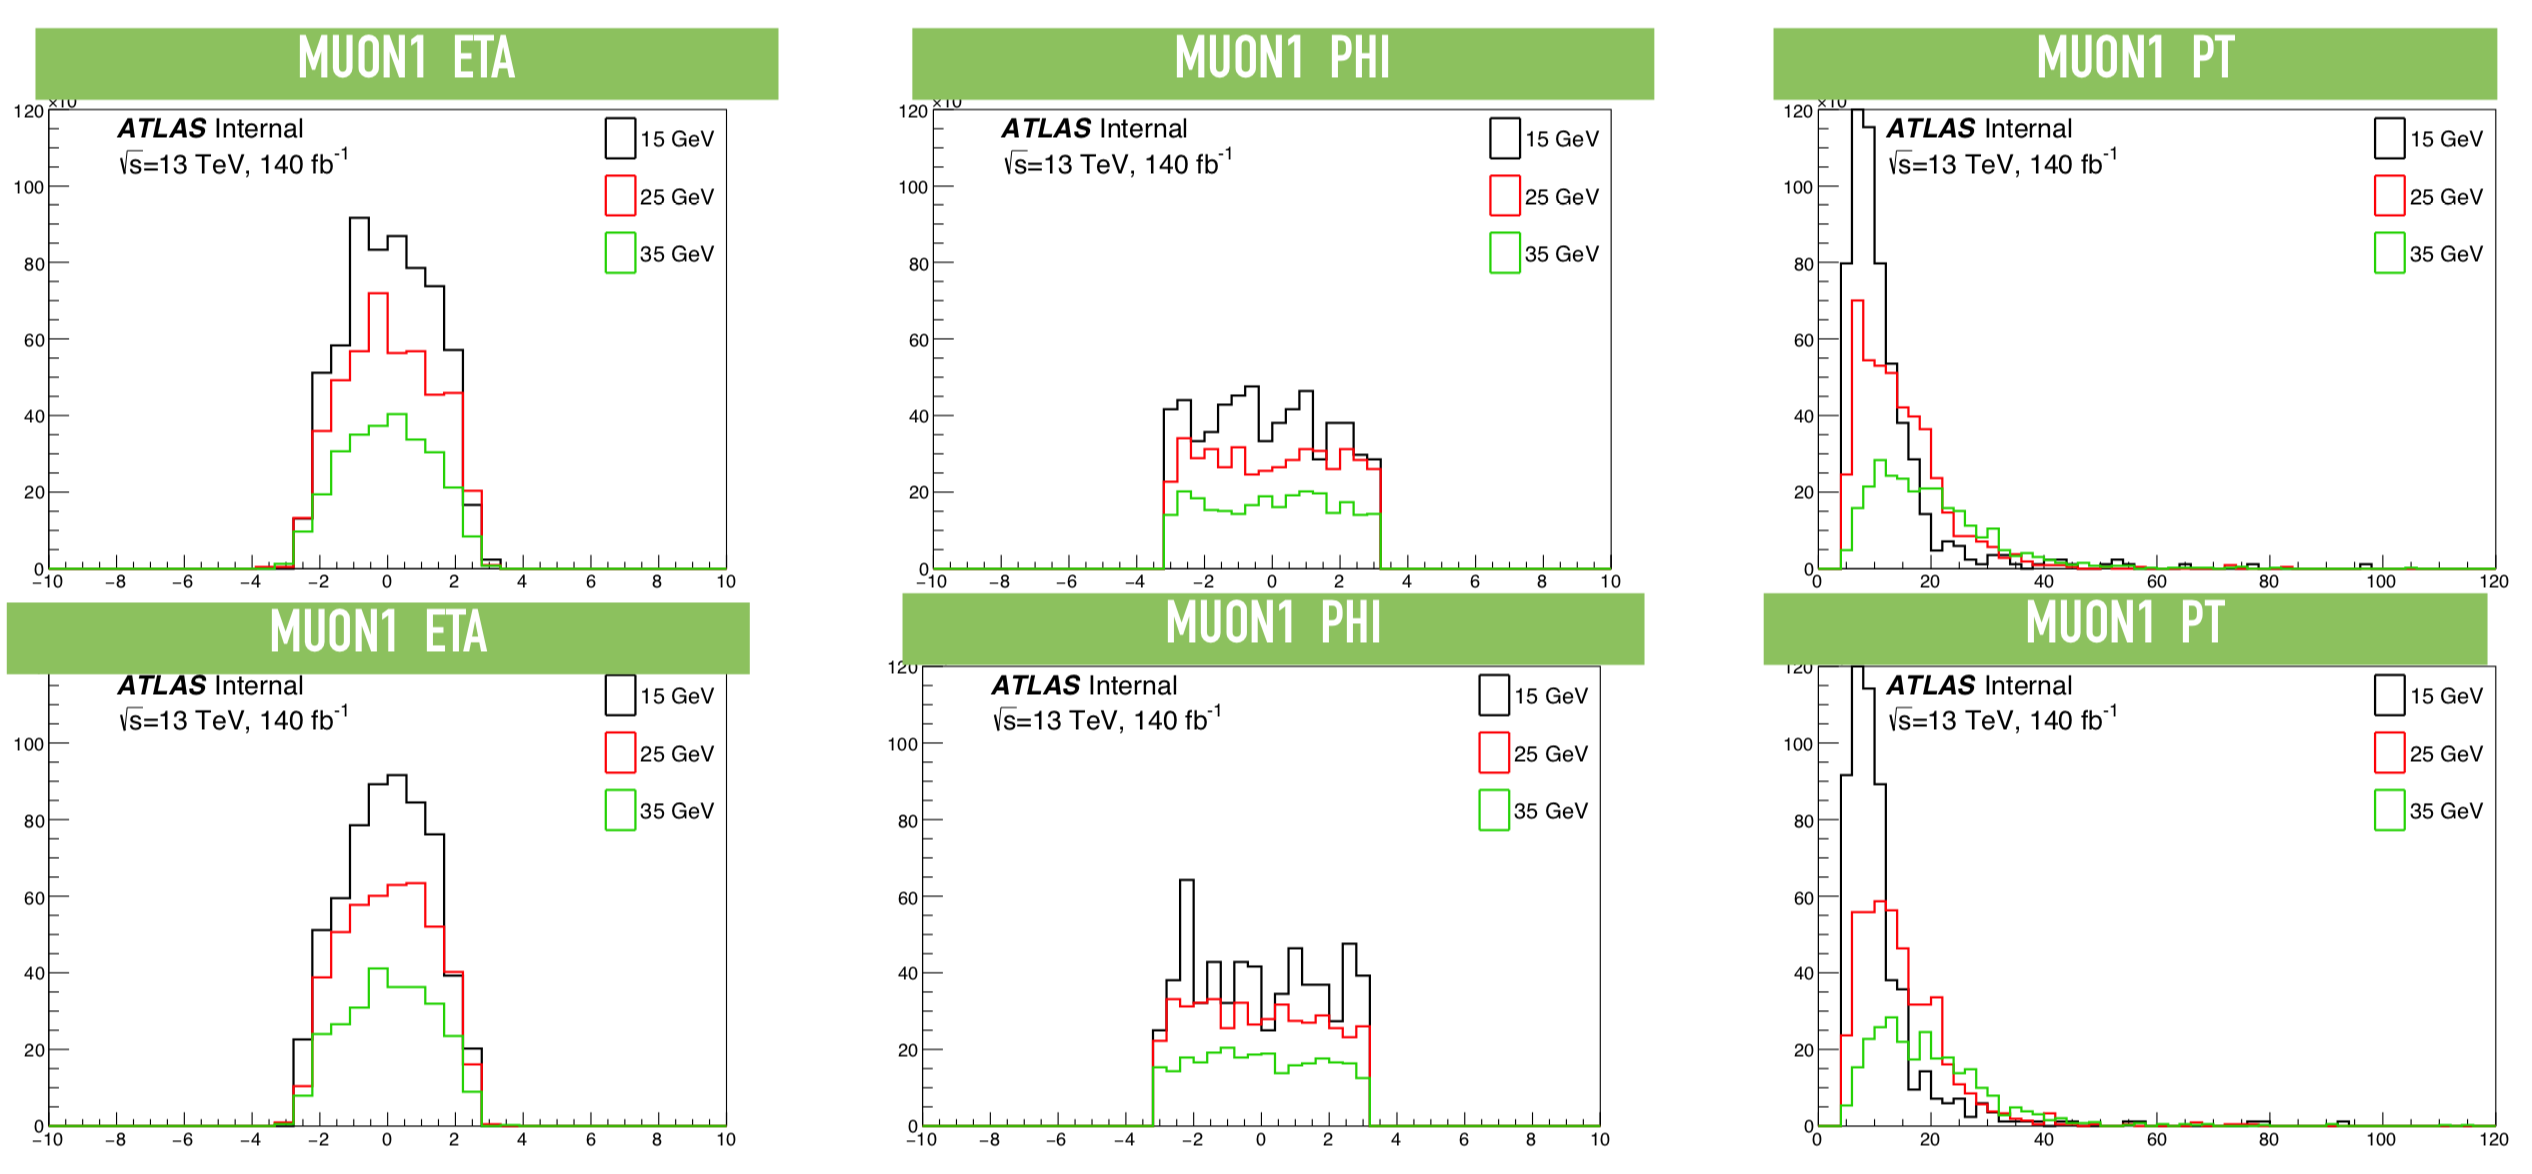
\includegraphics[width=0.75\textwidth]{figures/chapter_dimuon/dimuonISRdist1}
        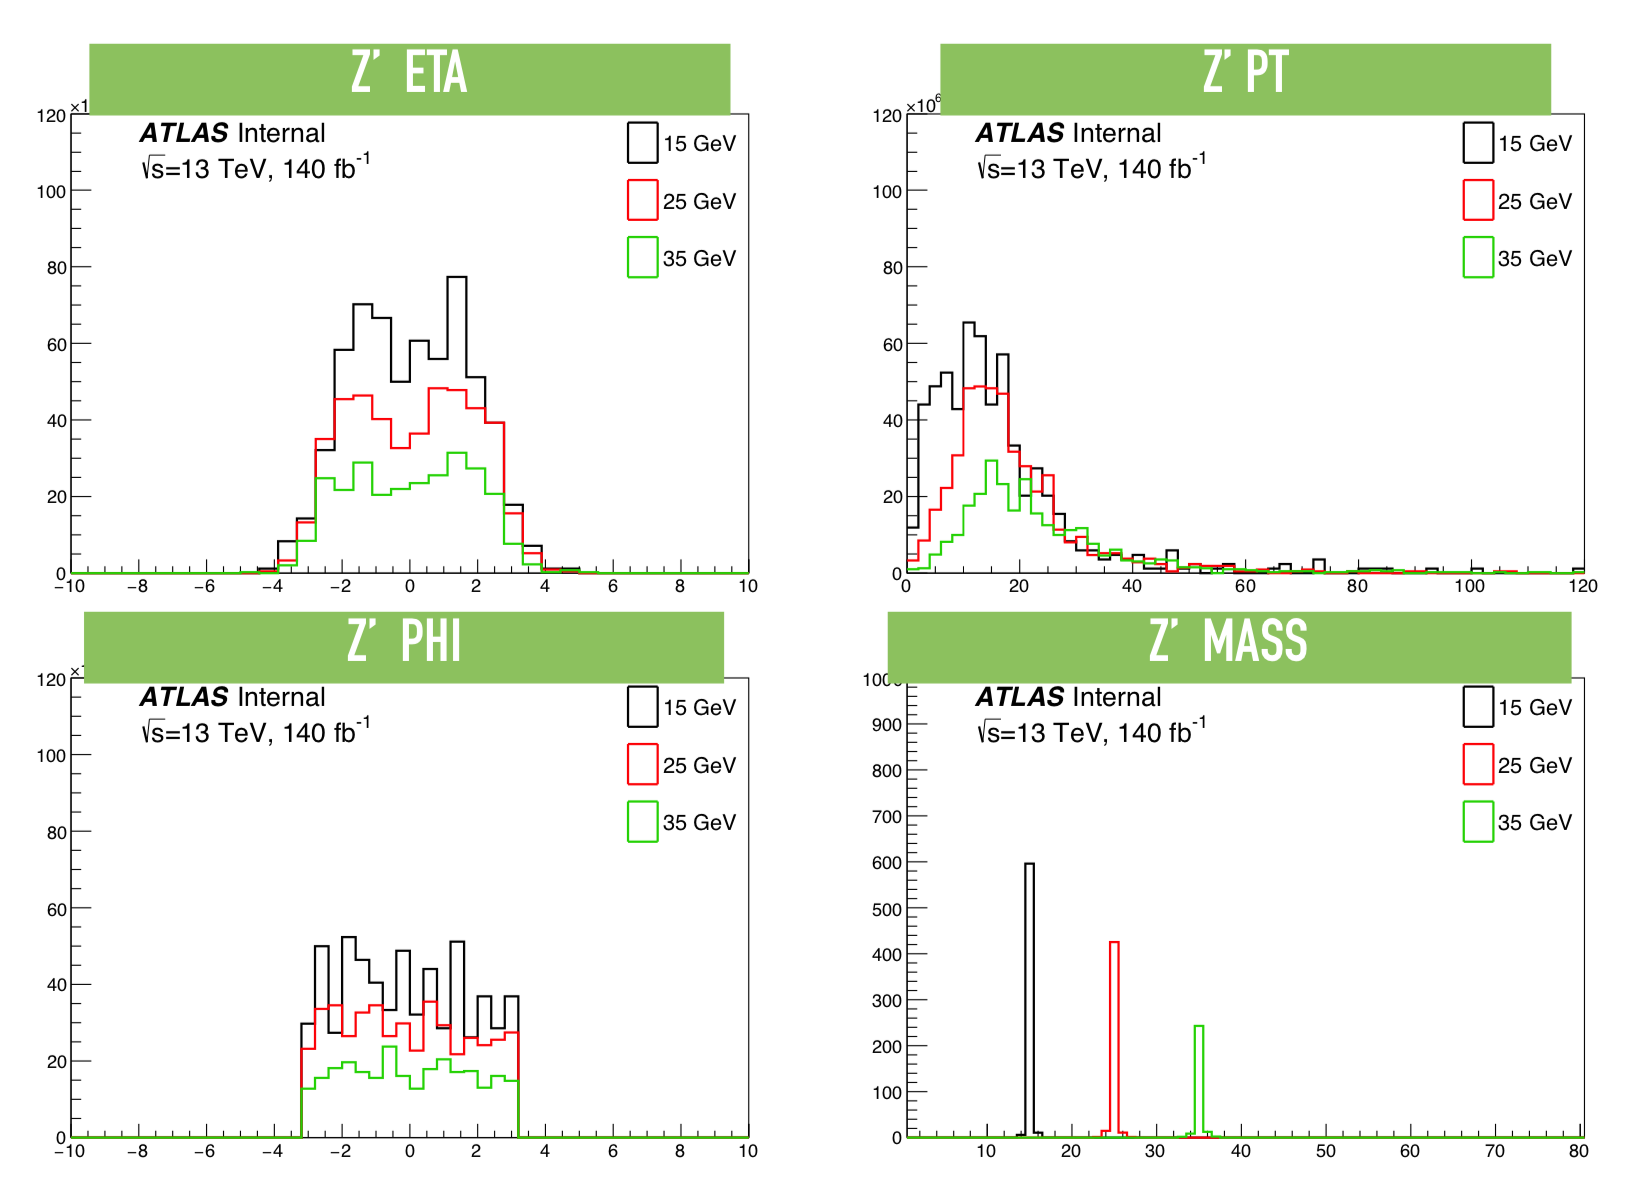
\includegraphics[width=0.5\textwidth]{figures/chapter_dimuon/dimuonISRdist2}
        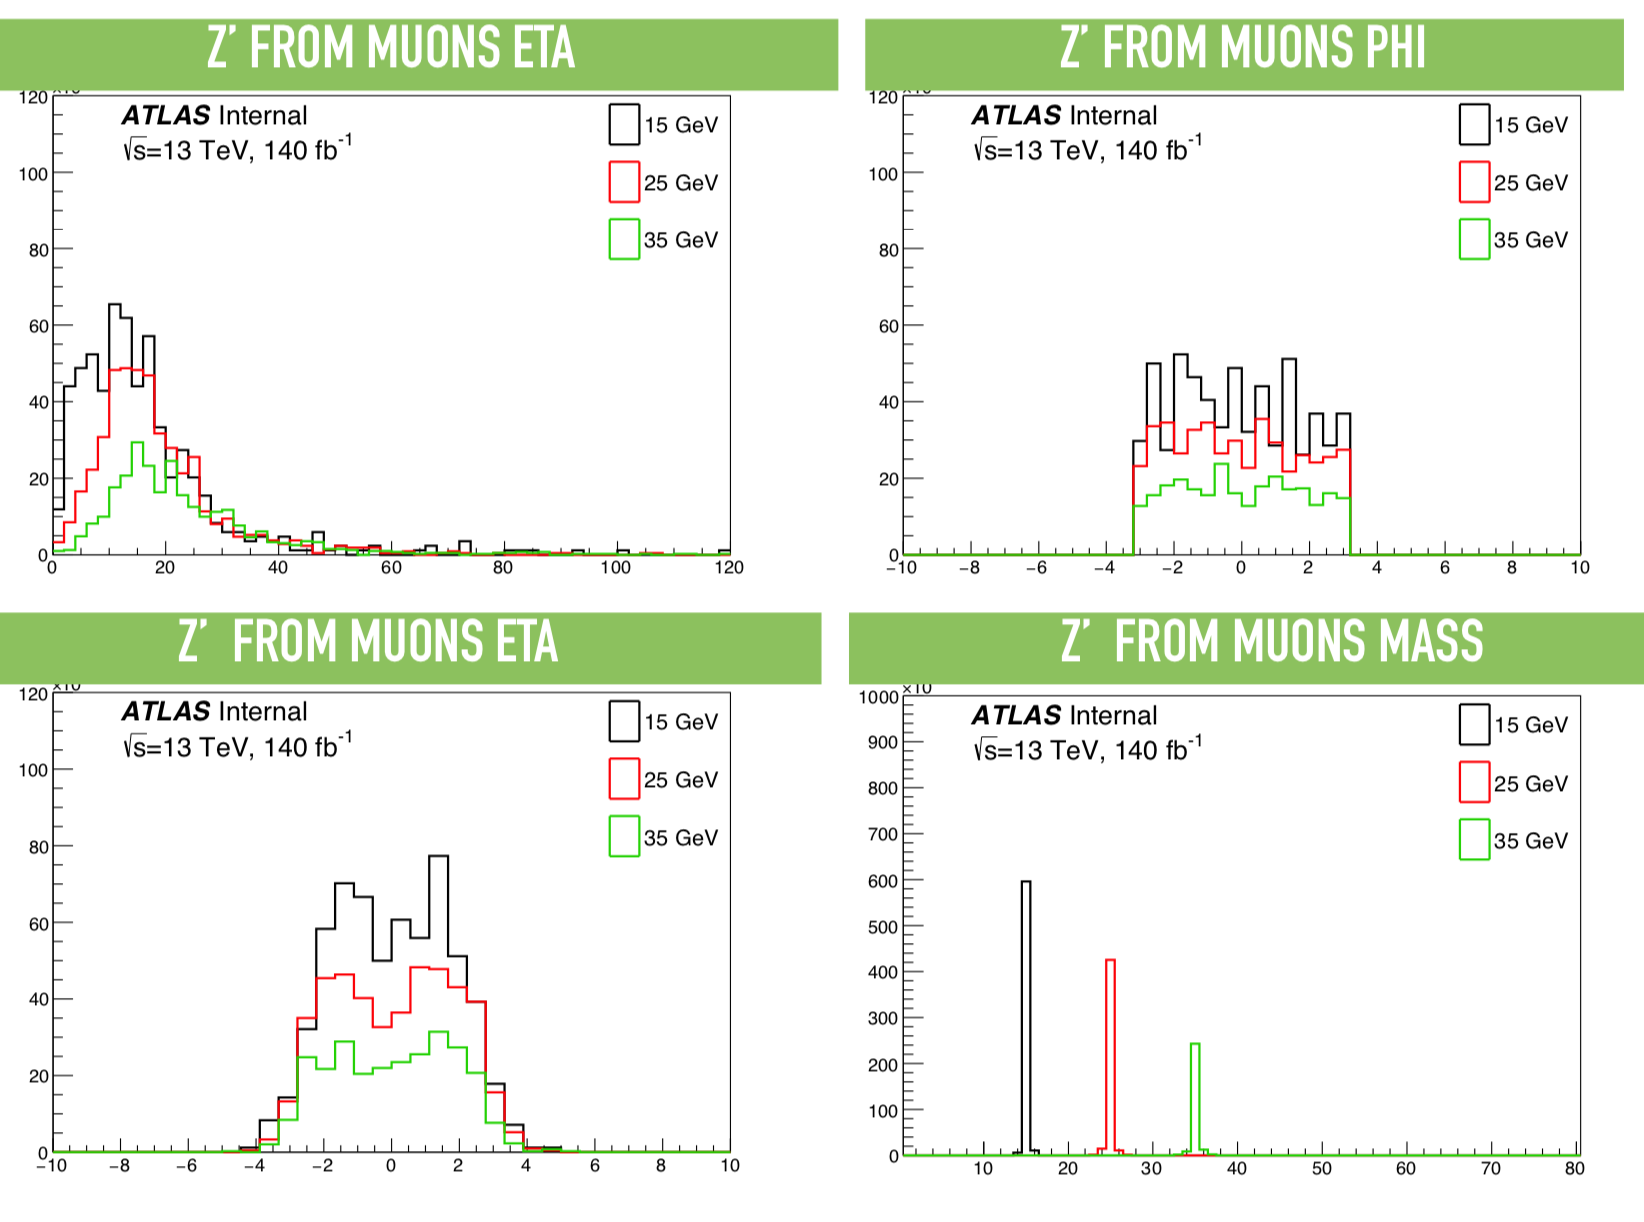
\includegraphics[width=0.5\textwidth]{figures/chapter_dimuon/dimuonISRdist3}
        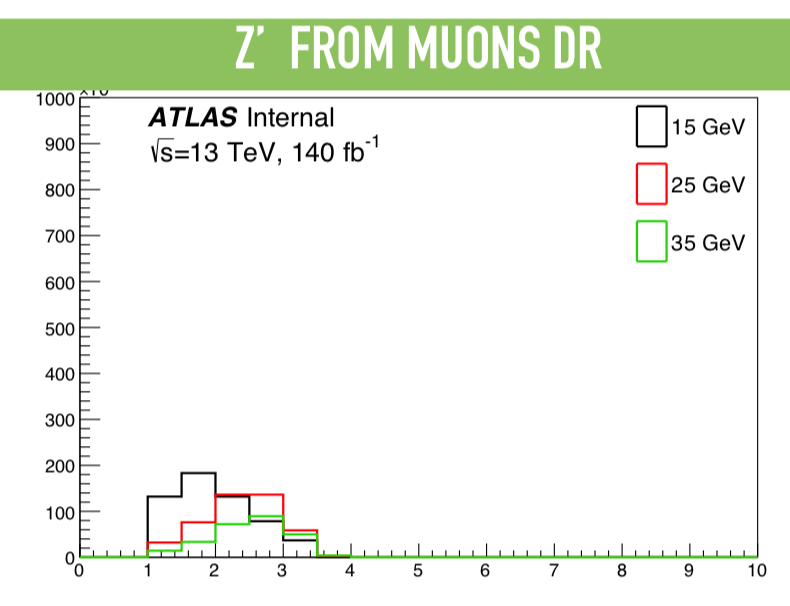
\includegraphics[width=0.2\textwidth]{figures/chapter_dimuon/dimuonISRdist4}
        \caption{
        This figure shows the signal distribution of the boosted dimuon samples generated. A minimal cut of muon pt >14 gev are done on the two leading muons. }
       \label{fig:boosted}
    \end{center}
\end{figure}


\section{Data preparation}

\subsection{Samples Used for the Analysis}
The following are the samples used for the analysis.

\begin{table}[!htb]
    \begin{center}
    \caption{
        The table shows the Monte Carlo dataset used for the analysis. 
    }
\label{tab:MC samples}
\begin{tabular}{|l|l|}
\hline
\textbf{MC Type}   & \textbf{DSID}                                                         \\ \hline
Z+ jets $\mu\mu$   & 364100 - 364113 , 364198-364203                                       \\ \hline
Z+jets $\tau \tau$ & 364128 - 364141 , 364210-364215                                       \\ \hline
$t\bar{t}$         & 410472                                                                \\ \hline
Diboson Sherpa     & 364253 - 364255 , 363355 - 363360 ; 363489 ; 364250 ; 364288 - 364290 \\ \hline
Top decay          & 410644 - 410645 , 410658 - 410659 ; 410648 - 410649                   \\ \hline
W + jets munu      & 364156 - 364169                                                       \\ \hline
$b\bar{b}$         & 363833                                                                \\ \hline
$c\bar{c}$         & 363834                                                                \\ \hline
\end{tabular}
\end{center}
\end{table}


\begin{table}[!htb]
    \begin{center}
    \caption{
        The table shows the Data dataset used for the analysis. 
    }
\label{tab:MC samples}
\begin{tabular}{|l|l|}
\hline
\textbf{Data Taking year}   & \textbf{Data Period} \\ \hline
2015   & D-J                                       \\ \hline
2016   & A-L                                       \\ \hline
2017   & B-F, H                                    \\ \hline
2018   & B-F, I, K, L-O, Q                         \\ \hline
\end{tabular}
\end{center}
\end{table}


\subsection{Trigger Chain}
The analysis takes the "OR" of the three trigger chains :

\begin{itemize}
    \item{HLT_2mu14}
    \item{HLT_mu22_mu8noL1}
    \item{HLT_mu26_ivarmedium}
\end{itemize}

\begin{figure}[!htb]
    \begin{center}
        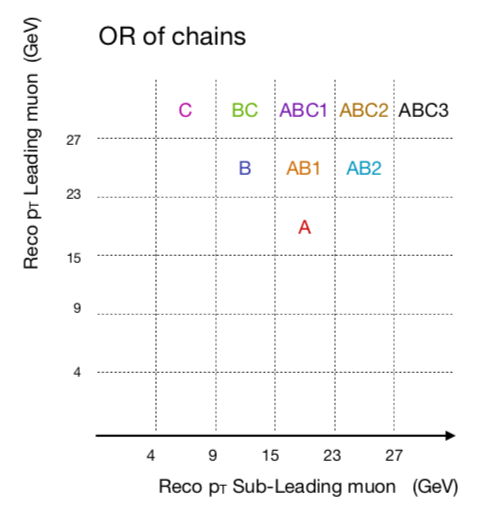
\includegraphics[width=0.75\textwidth]{figures/chapter_dimuon/TriggerChain}        
        \caption{
        This cartoon illstrate the trigger used for the different trigger region. A is HLT_2mu14, B represents HLT_mu22_mu8noL1; C shows HLT_mu26_ivarmedium. }
    \end{center}
\end{figure}

%The efficiency are calculated for each region for the subsequent weighting of in the trigger scale factor.
%\begin{equation}
%    SF= \epsilon_{data}/\episilon_{MC}
%\end{equation}

\subsection{Background composition}
The background composition of the Monte Carlo is shown here:

\begin{figure}[!htb]
    \begin{center}
        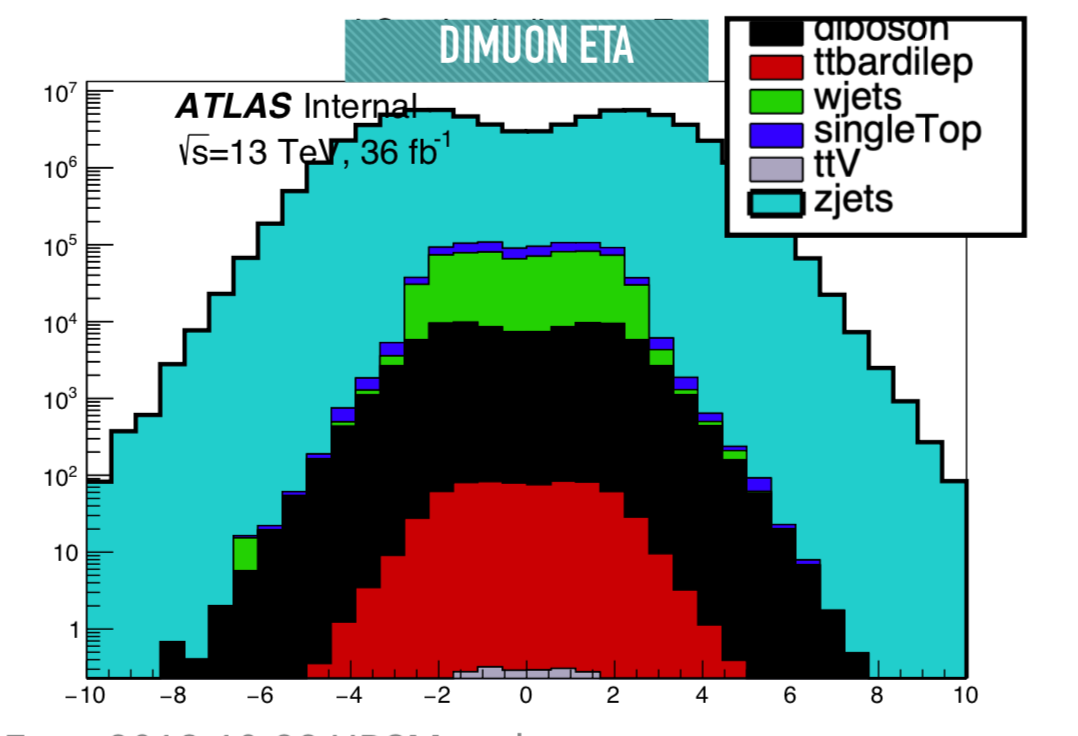
\includegraphics[width=0.75\textwidth]{figures/chapter_dimuon/backgroundcomposition}
        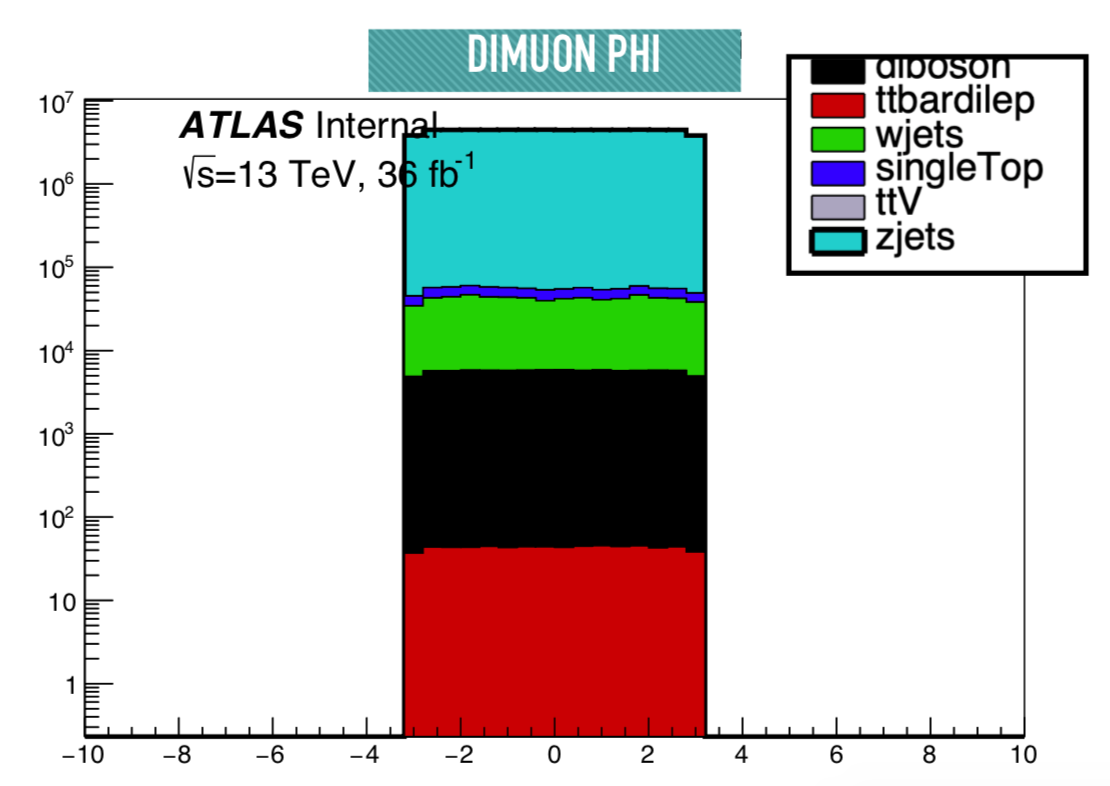
\includegraphics[width=0.75\textwidth]{figures/chapter_dimuon/backgroundcomposition2}
        \caption{
        This cartoon illstrate the background composition of the samples }
    \end{center}
\end{figure}

\subsection{Event Selection}
Following the above trigger cuts, the following event selections are made on the muons:

\subsubsection*{Muon Working Point}
The medium working point is chosen for the muons, details to the working point can be found here: 

The choice is made on the medium working point over low PT, as the trigger threshold effectively cut out most muons below 8GeV. The Low PT working point only has a higher efficiency over the medium working point below  6 GeV. 

\subsubsection*{Isolation Working Point}
FixedCutPflowLoose is chosen to be the isolation working point, details on the working point description can be found here:~\ref{}. 


\subsubsection{Fake Estimation}
Fakes are objects that are not opposite signed dimuon pairs that falls into the selection requirement in data event selection due to misidentifications.
Since the fakes mainly comes from QCD ATLAS processes, the amount from same signed process and opposite signed process are approximately the same. 
Fakes in the background sample can be estimated from the same signed leptons in data. Studies found that the content is less than 1\% of all the background contribution. The estimated same signed leptons contribution is added to the MC background composition.

\begin{figure}[!htb]
    \begin{center}
        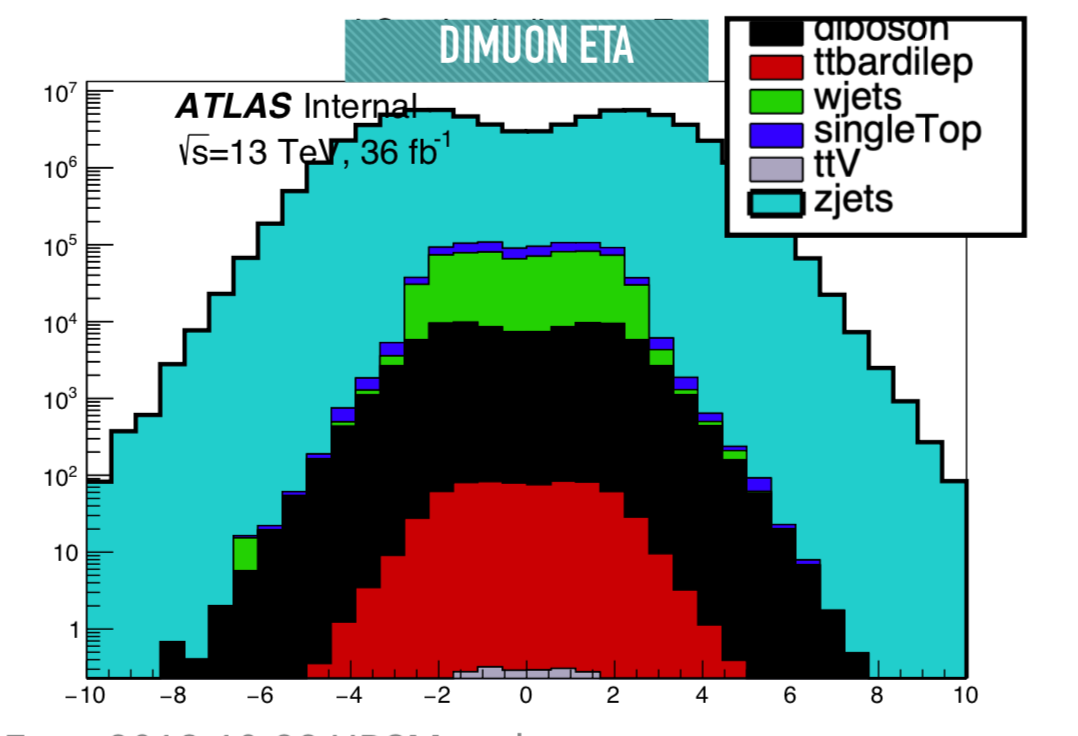
\includegraphics[width=0.75\textwidth]{figures/chapter_dimuon/backgroundcomposition}
        \caption{
        This cartoon illstrating the amount of fakes in the background composition. SS refers to same signed lepton in the data sample set, whereas OS refers to the opposite sign lepton pairs in data. }
    \end{center}
\end{figure}

\subsubsection{Superfast dimuon samples}
Due to the low statistics in the primary background sample in  Z > \mu \mu, fast generation relying on Pythia8 and a smearing function for the detector effect has been used to lower the statistical fluctuation. More details on the fast simulation can be found in the Higgs to $\mu \mu $ int note.

%\subsection{Sensitivity Test}
%Sensitivity test is done on the 

\subsection{Dimuon Mass Spectrum Resolution}
The mass spectrum resolution are done on the Powheg samples of Z > $\mu \mu
$. A Gaussian distribution fit is performed on the resonance mass $m_{\mu\muTruth} - m_{\mu\muReco}$ quantity. From the fit, the width of the Gaussian is obtained~\ref{fig:fit}, and is shown to follow the following distribution in figure~\ref{fig:sigma}.

\begin{figure}[!htb]
    \begin{center}
        \includegraphics[width=0.75\textwidth]{figures/chapter_dimuon/fitError}        
        \caption{
            A Gaussian distribution fit is made on the the difference between the truth dimuon resonance mass and the reconstructed dimuon resonance mass. }
    \end{center}
\end{figure}
   
\begin{figure}[!htb]
    \begin{center}
        \includegraphics[width=0.75\textwidth]{figures/chapter_dimuon/sigma}        
        \caption{
        From the fitted Gaussian distribution, the width is obtained for different resonance mass. They are plotted here. The width-to-mass resolution $\sigma_{m_{\mu\mu}}/m_{\mu\mu}$ is found to be close to 1.5\%.}
    \end{center}
\end{figure}


\subsection{Binning Strategy}
Using the resolution of the study from the last section and the mass distribution given in the theoretical signal section, the overall binning is chosen to be 0.25 GeV, it will allow for all signal searched for to be at least 2 bin wide. Signal that are at least two bin wide are significantly less prone to accidental "discoveries" due to statistical fluctuation.

\subsubsection{MC/Data Comparison}
A detailed description on the MC/Data comparison test can be found here,\ref{sec:MCData}.  
The agreement is shown to be good between the prepared MC and data. It shows that the MC is ready to be used for the subsequent tests.

\begin{figure}[!htb]
    \begin{center}
        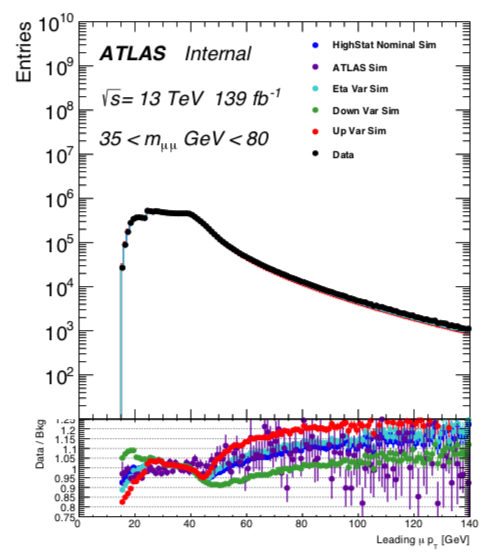
\includegraphics[width=0.75\textwidth]{figures/chapter_dimuon/MCDataCompare}
        %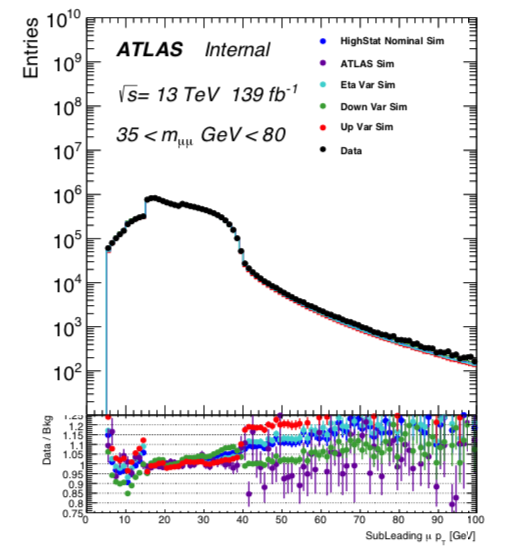
\includegraphics[width=0.75\textwidth]{figures/chapter_dimuon/MCDataCompare2}
        %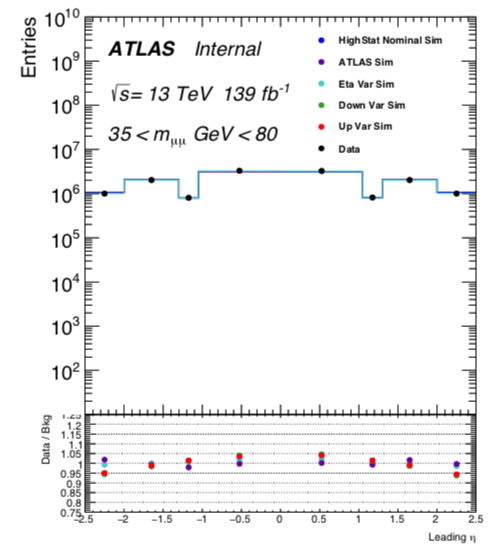
\includegraphics[width=0.75\textwidth]{figures/chapter_dimuon/MCDataCompare3}
        %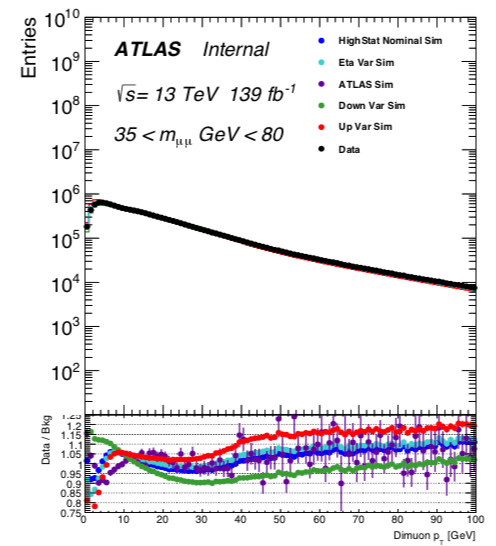
\includegraphics[width=0.75\textwidth]{figures/chapter_dimuon/MCDataCompare4}
        %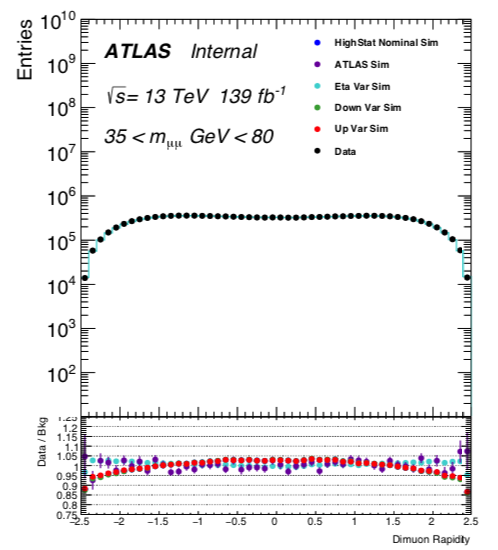
\includegraphics[width=0.75\textwidth]{figures/chapter_dimuon/MCDataCompare5}
        \caption{
        Monte Carlo and data comparison. A reasonable agreement is seen. Showing that the MC is ready to be used for the subsequent studies.
        }
    \end{center}
\end{figure}

\section{Background Fitting}

The Gaussian process background fitting method is being used for this study, a back-up fit function method is also used. Details on how these methods are motivated can be found here~\ref{section:backgroundest}.  

\subsection{Gaussian Process}

The Gaussian process background and signal kernels are given as cited here~\ref{sec:kernel}.

The minimum background lengthscale is studied through the signal injection test described here~\ref{signalInjection}.

Signal of mass widths of 1\%, 3\% and 5\% of different sizes are injected into the mass spectrum. It's found that a minimum lengthscale of 4 GeV is needed for the background kernel for the background model to be sensitive to signal of 3\sigma background error size and above.


\subsubsection{Signal injection test}
\begin{figure}[!htb]
    \begin{center}
        \includegraphics[width=0.75\textwidth]{figures/chapter_dimuon/signalInjection}        
        \caption{
        This figure illustrate a signal injection test performed at the mass point  }
            \label{fig:dimuonstudies}
    \end{center}
\end{figure}

\subsubsection{Background Modelling}
Using the minimal lengthscale chosen for the background and allowing other hyperparameters to float, tests fits are performed on the nominal fit, and also done on the different statistical variation of the background, the 1 $\sigma$ up and 1 $\sigma$ down variation of the fast simulation Pythia, as well as the $\eta$ variation.
The fitting result shows that Gaussian Process works well for all of these statistical variations. 

\begin{figure}[!htb]
    \begin{center}
        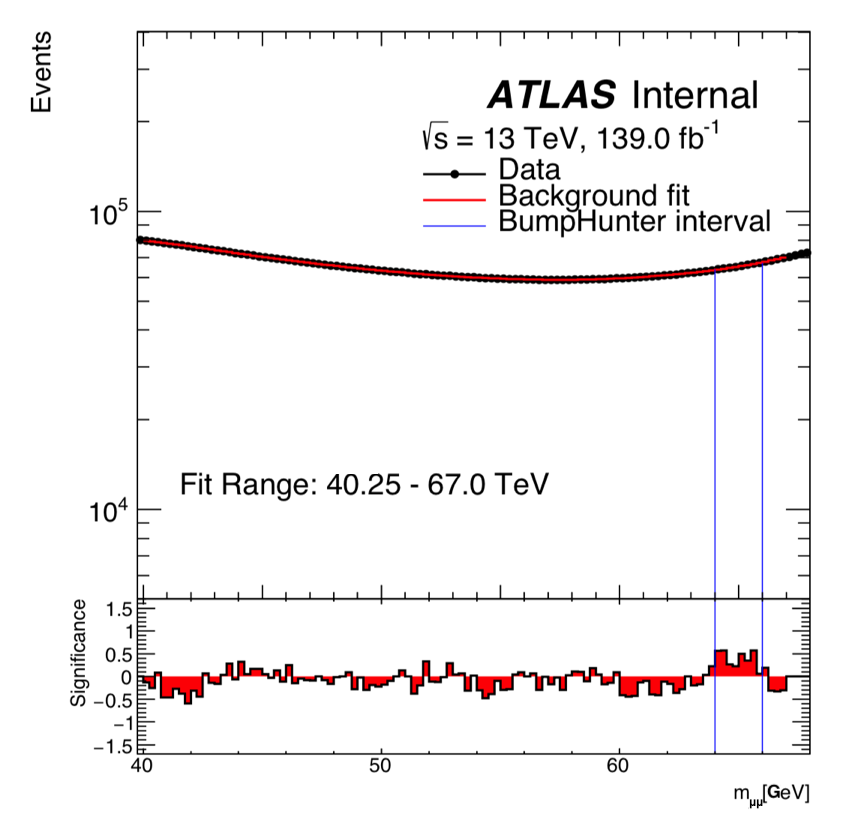
\includegraphics[width=0.75\textwidth]{figures/chapter_dimuon/Nominal}        
        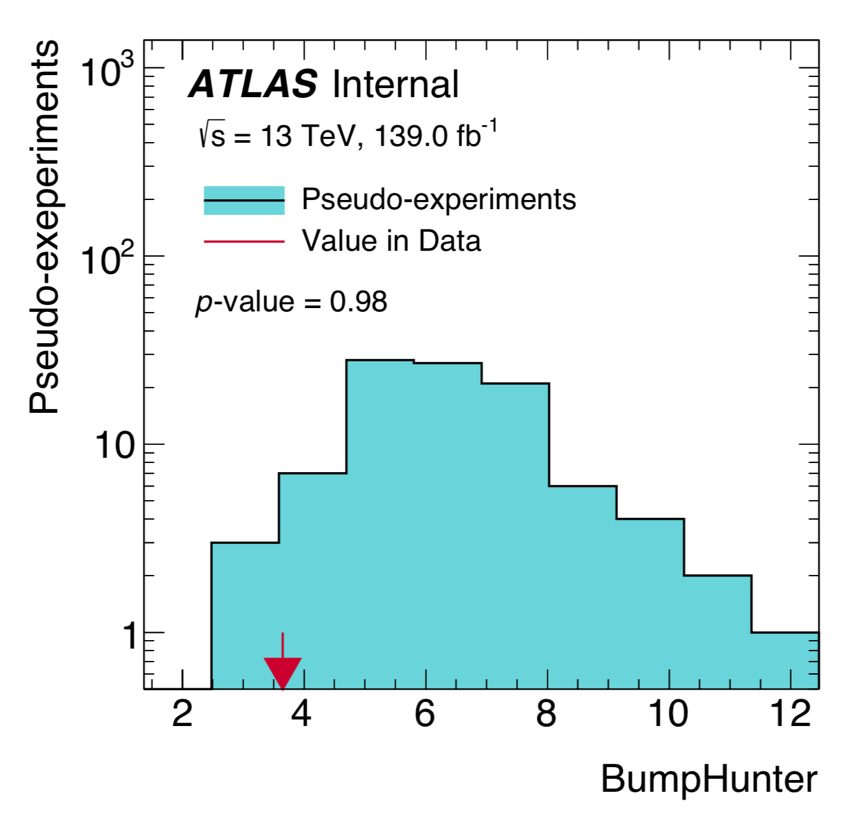
\includegraphics[width=0.75\textwidth]{figures/chapter_dimuon/NominalBH}        
        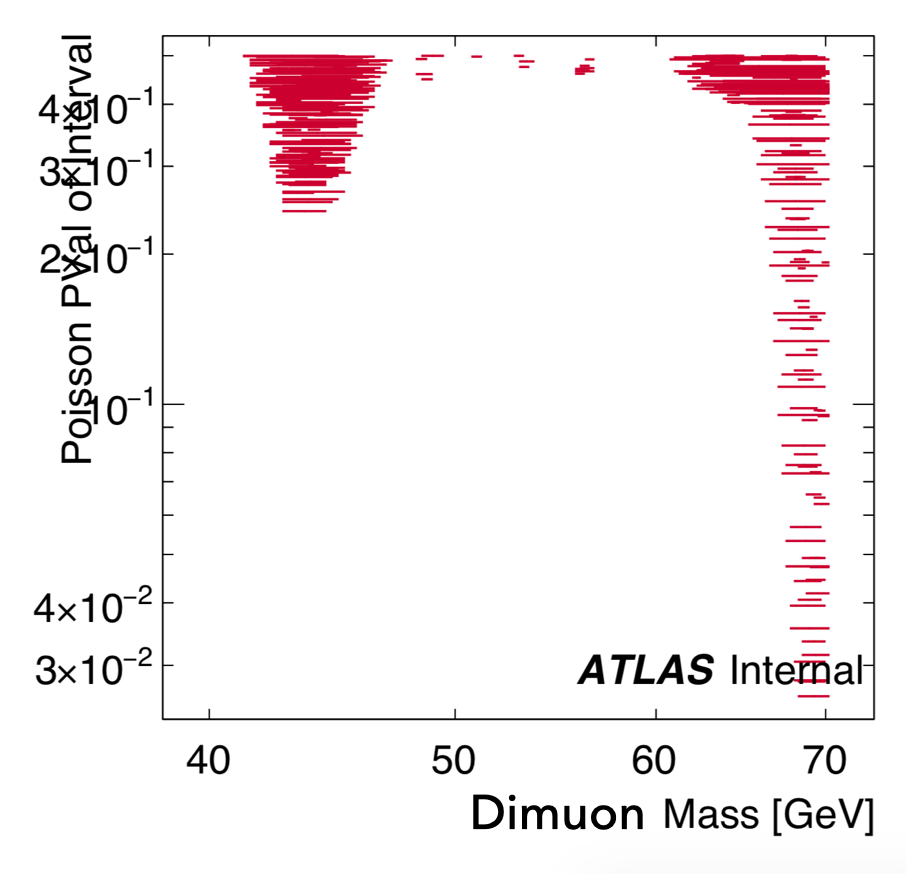
\includegraphics[width=0.75\textwidth]{figures/chapter_dimuon/NominalFit}        
        \caption{
        These figure illustrates the nominal fit, along with the bumphunter test statistics and the observed value distribution. It's shown that the most discrepant window does not fall below the critical p-value of 0.01. Details on the bumphunting procedure can be found here. }
            \label{fig:dimuonstudies}
    \end{center}
\end{figure}


\begin{figure}[!htb]
    \begin{center}
        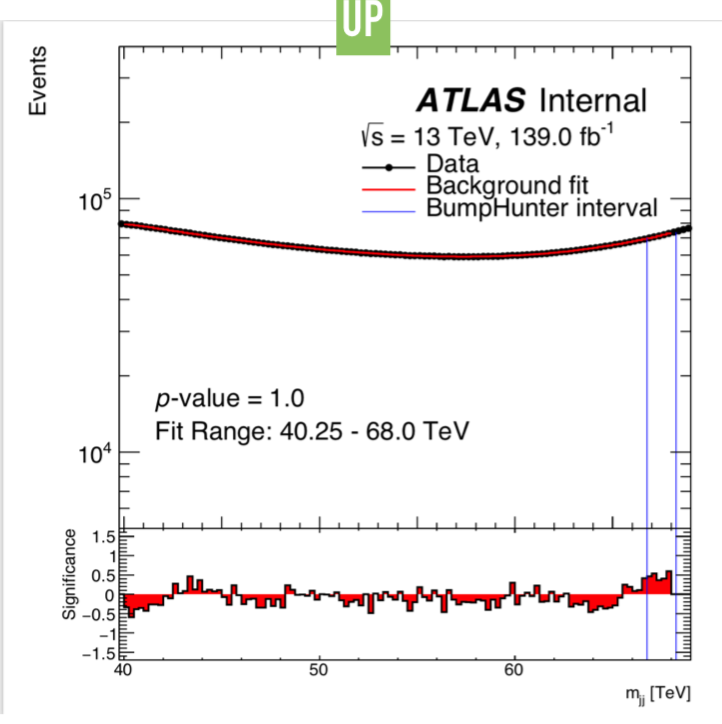
\includegraphics[width=0.75\textwidth]{figures/chapter_dimuon/UpVariation}
        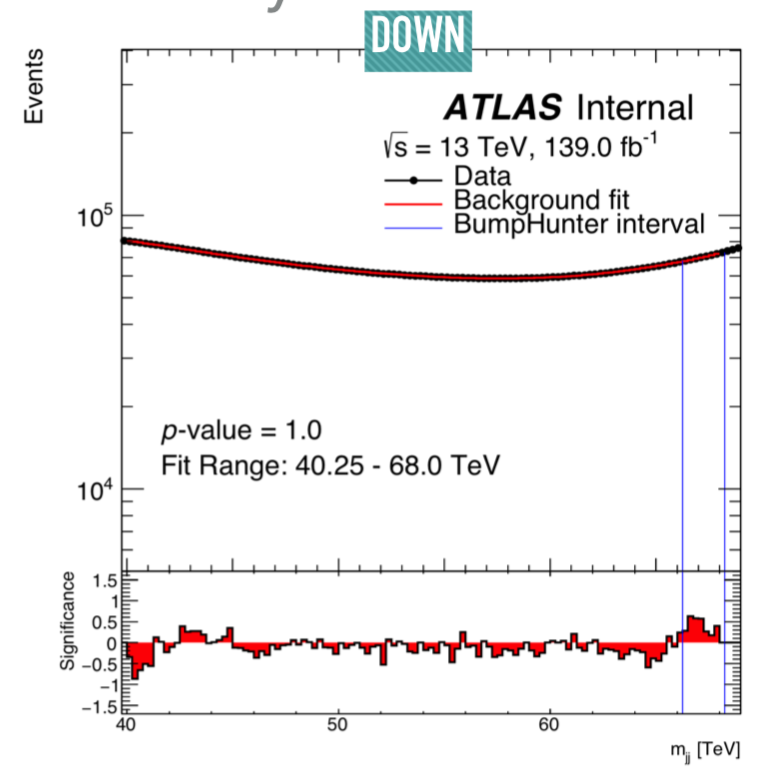
\includegraphics[width=0.75\textwidth]{figures/chapter_dimuon/DownVariation}
        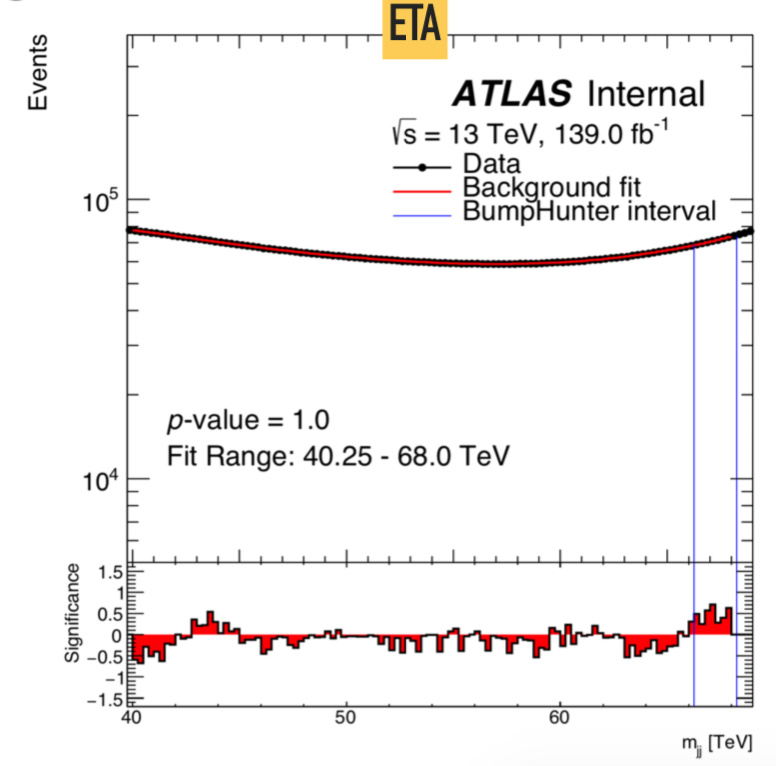
\includegraphics[width=0.75\textwidth]{figures/chapter_dimuon/EtaVariation}
        \caption{
        These figure illustrates the Gaussian Process background fits on the different variation of the MC generated. }
    \end{center}
\end{figure}



\subsection{Spurious signal test}
Details on the spurious signal can be found here~\ref{spurious}.
The spurious signal test results on the Gaussian process is shown here:

\begin{figure}[!htb]
    \begin{center}
        \includegraphics[width=0.75\textwidth]{figures/chapter_dimuon/spurious}        
        \caption{
        This figure illustrate a spurious signal test result on the different background variation fits.}
            \label{fig:dimuonstudies}
    \end{center}
\end{figure}


\section{Statistics Testing}
Details on the statistical test can be found here~\ref{}. During the time where the thesis was written, the data was not unblinded. Monte Carlo studies were done. A sample signal is injected into the spectrum to test the bumphunter, and the limit is generated using background MC assuming no signal was found.

\section{The Search}
A sample signal the size of 3$\sigma$ background error is injected into the spectrum, the test is done to illustrate that the search is capable of picking out the signal.
    


\begin{figure}[!htb]
    \begin{center}
        \includegraphics[width=0.75\textwidth]{figures/chapter_dimuon/signalinjected}
        \includegraphics[width=0.75\textwidth]{figures/chapter_dimuon/signalinjected2}
        \caption{
        These figures illustrate a test done on signal injected at 55 GeV, and the window exclusion that picked out the signal injected in there.}
%            \label{fig:dimuonstudies}
    \end{center}
\end{figure}

section{Limit Setting}
Preliminary limit setting is still currently under test, figure\ref{} shows a preliminary result from the Asimov method. 

begin{figure}[!htb]
   \begin{center}
       \includegraphics[width=0.75\textwidth]{figures/chapter_dimuon/limits}       
       \caption{
       This figure illustrate a spurious signal test result on the different background variation fits.}
            \label{fig:dimuonstudies}
   \end{center}
end{figure}

n alternative fit function limits calculated by approximation based on the fit function method is shown here, it's expected that the analysis will have comparible sensitivity to LHCb. 

begin{figure}[!htb]
   \begin{center}
       \includegraphics[width=0.75\textwidth]{figures/chapter_dimuon/limits}
       \caption{
       This figure illustrate a spurious signal test result on the different background variation fits.}
            \label{fig:dimuonstudies}
   \end{center}
end{figure}



section{Future Work}
he analysis is on its way to completing the final strategies and to be unblinded on data soon.

\section{Alternative fitting}
An alternative fitting method is done through the fit function method.

\section{Systematics}
section{Future Extensions}



\chapter{Future Resonance Finding}
\label{chapter:weird}

0. Introduction

1. Trigger level analysis

2. Future of resonance finding

3. Statisitcal method  


\chapter{Concluding Words: Anomalous Resonance as a Question}

%So tell me, what is it that I do not know?
%Anomalous resonances as a question to what can be looked for in physics
%A question in disguise
% add projected exclusion plot 

%I had a dream where I swallowed a cheerio shaped hole. 
%In a dream I swallowed a cheerio shaped hole.
%The question in the form of a bump.%
%This is not a search but rather a question in disguise. 
% Search claims thhat we actually do know someonthing about the bump.
% queer in search of joussance 

%\epigraph{\textit{The bud disappears when the blossom breaks through, and we might say that the former is refuted by the latter; in the same way when the fruit comes, the blossom may be explained to be a false form of the plant’s existence, for the fruit appears as its true nature in place of the blossom. The ceaseless activity of their own inherent nature makes these stages moments of an organic unity, where they not merely do not contradict one another, but where one is as necessary as the other; and constitutes thereby the life of the whole.}}{--Georg Hegel}

Particle physics has come a long way since its early days. Since the discovery of the Higgs Boson in 2012, the Standard Model is considered completed. But human's quest to understand fundamental physics is far from over. Many existing issues in Standard Model points to a picture out there unknown, yet to be understood. This evidence, especially those concerning Dark Matter, drove the resonance search analyses presented in Chapter~\ref{chapter:dijetISR} and Chapter~\ref{chapter:dimuon}.
However, as a highly distinguishable signature, resonances hunting offers much more than a tool to hunt for a specific candidate. In the age where most exotic and SUSY searches returned empty results, what ought to concern physicists regarding data is no longer merely what can be searched for, but also what can be \textit{asked}: what questions can be asked of data for them to reveal to us what we do not know? This chapter summarizes some directions that can be taken in the resonance hunting regime for future studies.
%But the search for the little bump is perhaps not just a search
%for dark matter, it is also a question on what is possible to be searched for and what lies between the boundaries of the known and unknown of our understanding. What is it that we do not know about? 


%Perhaps the gauge of what a physicist
%
%But human's search for truth is far from that.  However, along with all the compelling evidence, a complete physics theory is out there to be discovered. The analyses presented in Chapter~\ref{chapter:dijet} and Chapter~\ref{chapter:dimuon} both offered results important to answering of the question of Dark Matter. But in the age where new physics
%theory seems to be out of reach with most evidence, the quest of resonance hunting, is perhaps not merely to search for a theoretical candidate to what's out there. Is not in actuality a search, but rather, is a question in disguise. 
%What is possible for us to look for? The little bumps like signature is what lies between the known and the unknown of our understanding? Future lies in good miner and searcher for new things, it lies in physicists being good question askers in coaxing data from telling us its stories. 
%As a highly distinguishable signature, resonances not just a tool for catch, but also a question we can ask on what borders between the known and unknown. 
%
%the more compelling question that these analyses is no longer a particular theory candidate, but instead, to ask what is possible to be looked for?
%
%Instead the search for resonances, in their various methods, can be thought of as asking 
%
%the search for a more complete understanding to the nature of the world is far from over. One way to further our search is through these ripple nuggets of resonances. Driven by the question of Dark Matter, the analyses presented in Chapter~\ref{chapter:dijet} and Chapter~\ref{chapter:dimuon} bothoffers additional evidence to the search of the
%Dark Matter mediator Z'. The searches are also important in the following way, namely they extends beyond the previous ground and explored new tools for future resonance hunting effort. perhaps it's offering an alternative not just in the search but also in the method itself. Instead of 
%what is it possible to be looked for? 


%Figure here shows the dark matter exclusion limit plots from the dark matter chapter.

\section{Unexplored Landscape of the Two Body Resonances}
Chapter~\ref{chapter:topo} explored uncovered two-body final states in resonance hunting in detail. The paper has since been superseded by newer results ~\cite{2020}. The surveys offer an overview of all two-body final states that are left unsearched for in collider physics that could provide a wealth of sources for possible places to look for new physics signatures.

\section{Gaussian Process as a Background Modeling Method}
The Gaussian Process-based background estimation method is currently being finalized in ATLAS with the dimuon analysis in Chapter~\ref{chapter:dimuon}. It provides a more flexible method better suited for high luminosity for smooth background modeling for other resonance hunting analyses where MC is limited. The method offers the advantage of being \textit{generalizable} for any final state with a smooth background estimation in the signal region. The method will be applicable to many other future analyses. 
%Gaussian Process can also be extended to perform searched in the 2-dimensional search space for increased signal sensitivity.

\section{Data Scouting}
Due to limited bandwidth, the trigger described in Chapter~\ref{chapter:dimuon} set a lower bound in the mass of the resonance that could be searched for. Searching for a signal with initial state radiation mitigates this but it also results in a lowered sensitivity to the signal. Data scouting is a method proposed to create a special triggering stream and object to mitigate the limit triggering bandwidth by storing only partial events. Only information directly related to the analysis will be
stored. Currently, the dimuon data scouting analysis is under study in ATLAS and will be a future area with promising improved sensitivity. 

\section{Anomaly Detection for Resonances with Machine Learning Method}
The concept of “model-independent” searches is not unfamiliar to LHC. Searches for new particles often include model-independent results in the form of excesses beyond certain statistical significance LHC also has its dedicated general search ~\cite{General2019}. However, these current approaches are not truly model-independent: they are either signal model-dependent in the sensitivity optimal kinematic cut for targeted search or LHC background dependent in the general search. Search
sensitivity is greatly diminished if the anomaly is not as predicted by the signal or background models. An improved method will instead teach data to perform optimal selection on its own based only on the anomaly observed in data. One recent proposal is the weakly supervised Classification Without Labels (CWoLa) hunting method~\cite{CWoLA2019}. This technique discards the usual supervised Signal-over-background (S/B) kinematic strategy, where the optimal selection is made based on
the maximal S/B ratio of a specific model combination. In utilizing CWoLa for resonance hunting, the bump-like signal produces a signal-rich center-band and signal-deprived side-bands optimal for optimal sensitivity kinematic cuts training. If a new particle is embedded in the dataset, CWoLa training will produce a selection cut that maximizes events in the central-band-bump without any underlying S/B model assumptions. The data is made to reveal surprising anomalies on its own from the data alone.
The existing two-quark final state resonance CWoLa search~\cite{CWOLA2020} to other final states including muons, photons, and other uncovered resonance signatures. While the dijet analysis has proven the feasibility of the method in ATLAS, many detailed technical aspects, further generalizations, and expansions into larger feature spaces must still be performed. The new analyses on muon and photon final states will go beyond the predecessor by focusing the training on additional features including
the jet substructure of the ISR jet. More complicated signal topologies, where the primary resonant decay object can be composite, can also be explored using simpler muon/photon final state objects. The CWoLa model-independent searches will serve as complementary additions to current physics analyses’ model-dependent and independent search methods, and it will push sensitivity into new regions with attuned understanding driven by the data itself. 

%otheer anomaly searches are driven by-%rthe. It could open a new chapter where data are made to tell the truth behind. 


%\include{sections/chapter1}
%\include{sections/chapter2}
%\include{sections/chapter3}
%\include{sections/chapter4}
%\include{sections/chapter5}
%\include{sections/chapter6}
%\include{sections/chapter7}
%\include{sections/chapter8}
%\include{sections/chapter9}
%\include{sections/chapter10}

% These commands fix an odd problem in which the bibliography line
% of the Table of Contents shows the wrong page number.
\clearpage
\phantomsection

% "References should be formatted in style most common in discipline",
% abbrv is only a suggestion.



% The Thesis Manual says not to include appendix figures and tables in
% the List of Figures and Tables, respectively, so these commands from
% the caption package turn it off from this point onwards. If needed,
% it can be re-enabled later (using list=yes argument).
\captionsetup[figure]{list=no}
\captionsetup[table]{list=no}


\addcontentsline{toc}{chapter}{Bibliography}
\printbibliography
%\bibliographystyle{unsrt}
%\bibliography{bib/references.bib}


% If you have an appendix, it should come after the references.
%\appendix

\chapter{Basics of Machine Learning}
\label{app:ml}



\end{document}
